\documentclass[12pt,a4paper,final]{book}
\usepackage[utf8]{inputenc}
\usepackage{graphicx}
\usepackage[italian]{babel}
\usepackage[a4paper, headheight=15mm, width=150mm,top=25mm,bottom=25mm,bindingoffset=6mm]{geometry}
\usepackage{fancyhdr}
\usepackage{xcolor}
\usepackage{adjustbox}
\usepackage{cite}
\usepackage[final]{pdfpages}
\definecolor{codegreen}{rgb}{0,0.6,0}
\definecolor{codegray}{rgb}{0.5,0.5,0.5}
\definecolor{codepurple}{rgb}{0.58,0,0.82}
\definecolor{backcolour}{rgb}{0.95,0.95,0.92}
\usepackage{listings}
\lstdefinestyle{mystyle}{
    commentstyle=\color{codegreen},
    keywordstyle=\color{magenta},
    numberstyle=\tiny\color{codegray},
    stringstyle=\color{codepurple},
    basicstyle=\ttfamily\footnotesize,
    breakatwhitespace=false,
    breaklines=true,
    captionpos=b,
    keepspaces=true,
    numbers=left,
    numbersep=5pt,
    showspaces=false,
    showstringspaces=false,
    showtabs=false,
    tabsize=2
}


\usepackage{stackengine}
\newcommand\xrowht[2][0]{\addstackgap[.5\dimexpr#2\relax]{\vphantom{#1}}}

\definecolor{DarkGreen}{rgb}{0.0,0.4,0.0}
\definecolor{Blue}{rgb}{0.0,0.0,0.0} % Comment color
\definecolor{highlight}{RGB}{236, 242, 248} % Code highlight color
\lstdefinestyle{Style1}{ % Define a style for your code snippet, multiple definitions can be made if, for example, you wish to insert multiple code snippets using different programming languages into one document
language=python, % Detects keywords, comments, strings, functions, etc for the language specified
backgroundcolor=\color{highlight}, % Set the background color for the snippet - useful for highlighting
basicstyle=\footnotesize\ttfamily, % The default font size and style of the code
breakatwhitespace=false, % If true, only allows line breaks at white space
breaklines=true, % Automatic line breaking (prevents code from protruding outside the box)
captionpos=b, % Sets the caption position: b for bottom; t for top
commentstyle=\usefont{T1}{pcr}{m}{sl}\color{DarkGreen}, % Style of comments within the code - dark green courier font
deletekeywords={}, % If you want to delete any keywords from the current language separate them by commas
%escapeinside={\%}, % This allows you to escape to LaTeX using the character in the bracket
firstnumber=1, % Line numbers begin at line 1
frame=single, % Frame around the code box, value can be: none, leftline, topline, bottomline, lines, single, shadowbox
 % Rounds the corners of the frame for the top left, top right, bottom left and bottom right positions
keywordstyle=\color{Blue}\bf, % Functions are bold and blue
morekeywords={}, % Add any functions no included by default here separated by commas
numbers=left, % Location of line numbers, can take the values of: none, left, right
numbersep=10pt, % Distance of line numbers from the code box
numberstyle=\tiny\color{Gray}, % Style used for line numbers
rulecolor=\color{black}, % Frame border color
showstringspaces=false, % Don't put marks in string spaces
showtabs=false, % Display tabs in the code as lines
stepnumber=5, % The step distance between line numbers, i.e. how often will lines be numbered
stringstyle=\color{Purple}, % Strings are purple
tabsize=4, % Number of spaces per tab in the code
}
% Create a command to cleanly insert a snippet with the style above anywhere in the document
\newcommand{\insertcode}[2]{\begin{itemize}\item[]\lstinputlisting[caption=#2,label=#1,style=Style1]{#1}\end{itemize}} % The first argument is the script location/filename and the second is a caption for the listing
\lstset{style=mystyle}
\pagestyle{fancy}
\fancyhf{}
\fancyhead[L]{\nouppercase{\leftmark}}
\fancyhead[R]{\thepage}
\linespread{1.2}
\usepackage{amsmath}
\usepackage{mathtools}
\usepackage{textcomp}
\usepackage{gensymb}
\usepackage{nccmath}
\usepackage{mathrsfs}
\usepackage{units} 
\usepackage{subcaption}
\usepackage{afterpage}
\usepackage{verbatim}
\usepackage{caption}
\usepackage[font=small,labelfont=bf]{caption}
\usepackage[pdfa]{hyperref}
%%%%%%%%%%%%%%%%%%%%%%%%%%%%%%%%%%%%%%%%%%%%%%%%%%%%%%%%
\title{Tesi di laurea triennale di Eleonora Gatti}
\author{Eleonora Gatti}
\date{Maggio/Luglio 2020}
%%%%%%%%%%%%%%%%%%%%%%%%%%%%%%%%%%%%%%%%%%%%%%%%%%%%%%%
%%%%%%%%%%%%%%%%%%%%%%%%%%%%%%%%%%%%%%%%%%%%%%%%%%%%%%%
%%%%%%%%%%%%%%%%%%%%%%%%%%%%%%%%%%%%%%%%%%%%%%%%%%%%%%%

\begin{document}

%%%%%%%%%%%%%%%%%%%%  PRIMA PAGINA  %%%%%%%%%%%%%%%%%%%


\includepdf[pages=-]{../frontespizio/frontespizio.pdf}
\newpage
\thispagestyle{empty}
\clearpage\mbox{}\clearpage
\newpage
\thispagestyle{empty}

%%%%%%%%%%%%%%%%%%%%%%%  INDICE  %%%%%%%%%%%%%%%%%%%%%

\tableofcontents
\newpage

%%%%%%%%%%%%%%%%%%%%  CAPITOLO 1  %%%%%%%%%%%%%%%%%%%%

\chapter{Sistemi ottici nelle microonde}\label{intro_sistemi_ottici}
Quasi tutta l'informazione che abbiamo a disposizione su oggetti astronomici molto distanti è contenuta nella radiazione elettromagnetica emessa. Per secoli l'unico tipo di analisi possibile è stata quella nello spettro del visibile. Oggigiorno esistono svariate branche dell'astrofisica che analizzano segnali provenienti dall'Universo a diverse frequenze elettromagnetiche; una di queste branche riguarda lo studio del cosmo attraverso le microonde. 

    %%%%%%%%%%%%%%%%%%%  CAPITOLO 1.1  %%%%%%%%%%%%%%%%%%%

\section{Utilizzo delle microonde in astrofisica}\label{microonde_astrofisica}
Il range delle lunghezze d'onda delle microonde è $\lambda \sim 1 \unit{mm} \div 10 \unit{cm}$\footnote{Il confine tra onde radio e microonde non è netto, spesso si parla di radio estendendo il range di lunghezze d'onda anche a quello delle microonde.}.


\`E estremamente importante fare osservazioni a grandi lunghezze d'onda, nel millimetrico e oltre, poiché esistono numerosissime sorgenti cosmologiche che emettono in questo range e possono essere analizzate tramite sistemi ottici nelle microonde.
I segnali più comunemente studiati in radio astronomia e attraverso le microonde sono:
\begin{itemize}
	\item radiazione emessa da gas ionizzato;
	\item radiazione di sincrotrone, dovuta al moto di particelle cariche libere di muoversi nell'Universo e deviate da campi magnetici;
	\item effetto Sunyaev-Zeldovich, che permette di rivelare ammassi di galassie altrimenti non visibili;
	\item emissioni del Sole;
	\item radiazioni da regioni H II; si tratta di regioni nello spazio in cui sono presenti stelle molto calde (di tipo O o di tipo B) che ionizzano il gas intorno ad esse il quale emette nelle microonde e nel radio;
	\item supernovae e resti di supernovae\footnote{La Crab Nebula, per esempio, è estremamente visibile nelle moicroonde.};
	\item pulsar;
	\item radio galassie;
	\item CMB.
\end{itemize}
In questo lavoro di tesi lo studio è stato effettuato su sistemi ottici ottimizzati per l'analisi della CMB.


La \textbf{CMB}, Cosmic Microwave Background, è la radiazione a microonde di fondo cosmico che permea l’intero Universo.
Secondo il \textit{Modello Cosmologico Standard (SCM)} l'Universo ha avuto origine circa $14$ miliardi di anni fa da una singolarità iniziale: il \textit{Big Bang}.
Nei primissimi istanti dopo il \textit{Big Bang} vi fu una rapidissima fase di espansione ($10^{-33}~\unit{s}$), detta \textit{inflazione}, seguita da un'espansione più lenta e regolare, che continua tutt'ora. Inizialmente materia e radiazione erano in equilibrio in un plasma estremamente caldo; la progressiva espansione ha causato un abbassamento della temperatura del plasma. L'equilibrio tra materia e radiazione venne a mancare quando la temperatura raggiunse $T \simeq 3000~\unit{K}$. Questo causò il \textit{disaccoppiamento} tra materia e radiazione: la maggior parte degli elettroni venne catturata dai nuclei atomici permettendo la formazione dei primi atomi neutri. Convenzionalmente si considera come tempo al quale si è verificato il \textit{disaccoppiamento} tra materia e radiazione l'istante $t_{dec}$ in cui il libero cammino medio dei fotoni divenne maggiore della scala dell'Universo osservabile. Questo accadde a circa $380~000~\unit{anni}$ dal \textit{Big Bang} e da allora i fotoni primordiali sono liberi di vagare nello spazio e sono i costituenti della radiazione a microonde di fondo cosmico.
Nell'ipotesi semplificata di un Universo non in espansione, i fotoni primordiali che possiamo osservare oggi dalla Terra sono quelli che all'istante $t_{dec}$ si trovavano ad una distanza $c(t_{now}-t_{dec})$; il che significa che per ogni istante un osservatore sulla Terra può osservare solo i fotoni emessi da un guscio sferico che prende il nome di \textit{Last Scattering Surface} (LSS). Generalizzando il caso ad un Universo in espansione il concetto rimane lo stesso ma diventa matematicamente più complesso. I fotoni della CMB che vengono oggi misurati rappresentano una radiazione quasi-isotropa il cui spettro è quello di corpo nero a una temperatura $T\approx2.73\unit{K}$. Per studiare le proprietà della CMB sulla sfera definita dalla LSS è utile utilizzare una decomposizione in \textit{armoniche sferiche} $Y_l^m(\theta,\phi)$. La decomposizione in armoniche sferiche di una funzione $f(\theta,\phi)$ su una sfera è data da:
\[f(\theta,\phi)=\sum_{\ell=0}^\infty\sum_{m=-\ell}^\ell a_{\ell m}Y_\ell^m(\theta,\phi)\]
dove $a_{\ell m}$ sono coefficienti complessi che contengono informazioni sia sull'ampiezza che sulla fase delle armoniche sulla sfera. Tuttavia, data l'arbitrarietà del sistema di riferimento che si utilizza quando si compie un'analisi statistica della CMB, la fase può essere trascurata; diventa quindi più interessante utilizzare la quantità: \[C_{\ell}=\langle a_{\ell m} a_{\ell m}^* \rangle\]
detta \textbf{spettro di potenza}. Nel caso di misura da parte di un solo strumento la media $\langle \cdot \rangle$ è effettuata su tutti i possibili valori di \textit{m}.


La radiazione della CMB è polarizzata e lo spettro di potenza della polarizzazione può essere decomposto in due componenti, dette \textit{modi E} e \textit{modi B}. Una misura dei modi B permetterebbe una verifica del paradigma dell'inflazione in quanto questi sarebbero generati da onde gravitazionali primordiali, e solo l'inflazione sarebbe in grado di espanderne le scale angolari fino a risoluzioni osservabili oggi.\footnote{In cosmologia \textit{r} è un parametro che prende il nome di rapporto tensore-scalare ed è definito come il rapporto tra la potenza dei modi B e dei modi E primordiali.}
\begin{figure}[!ht]
	\centering
	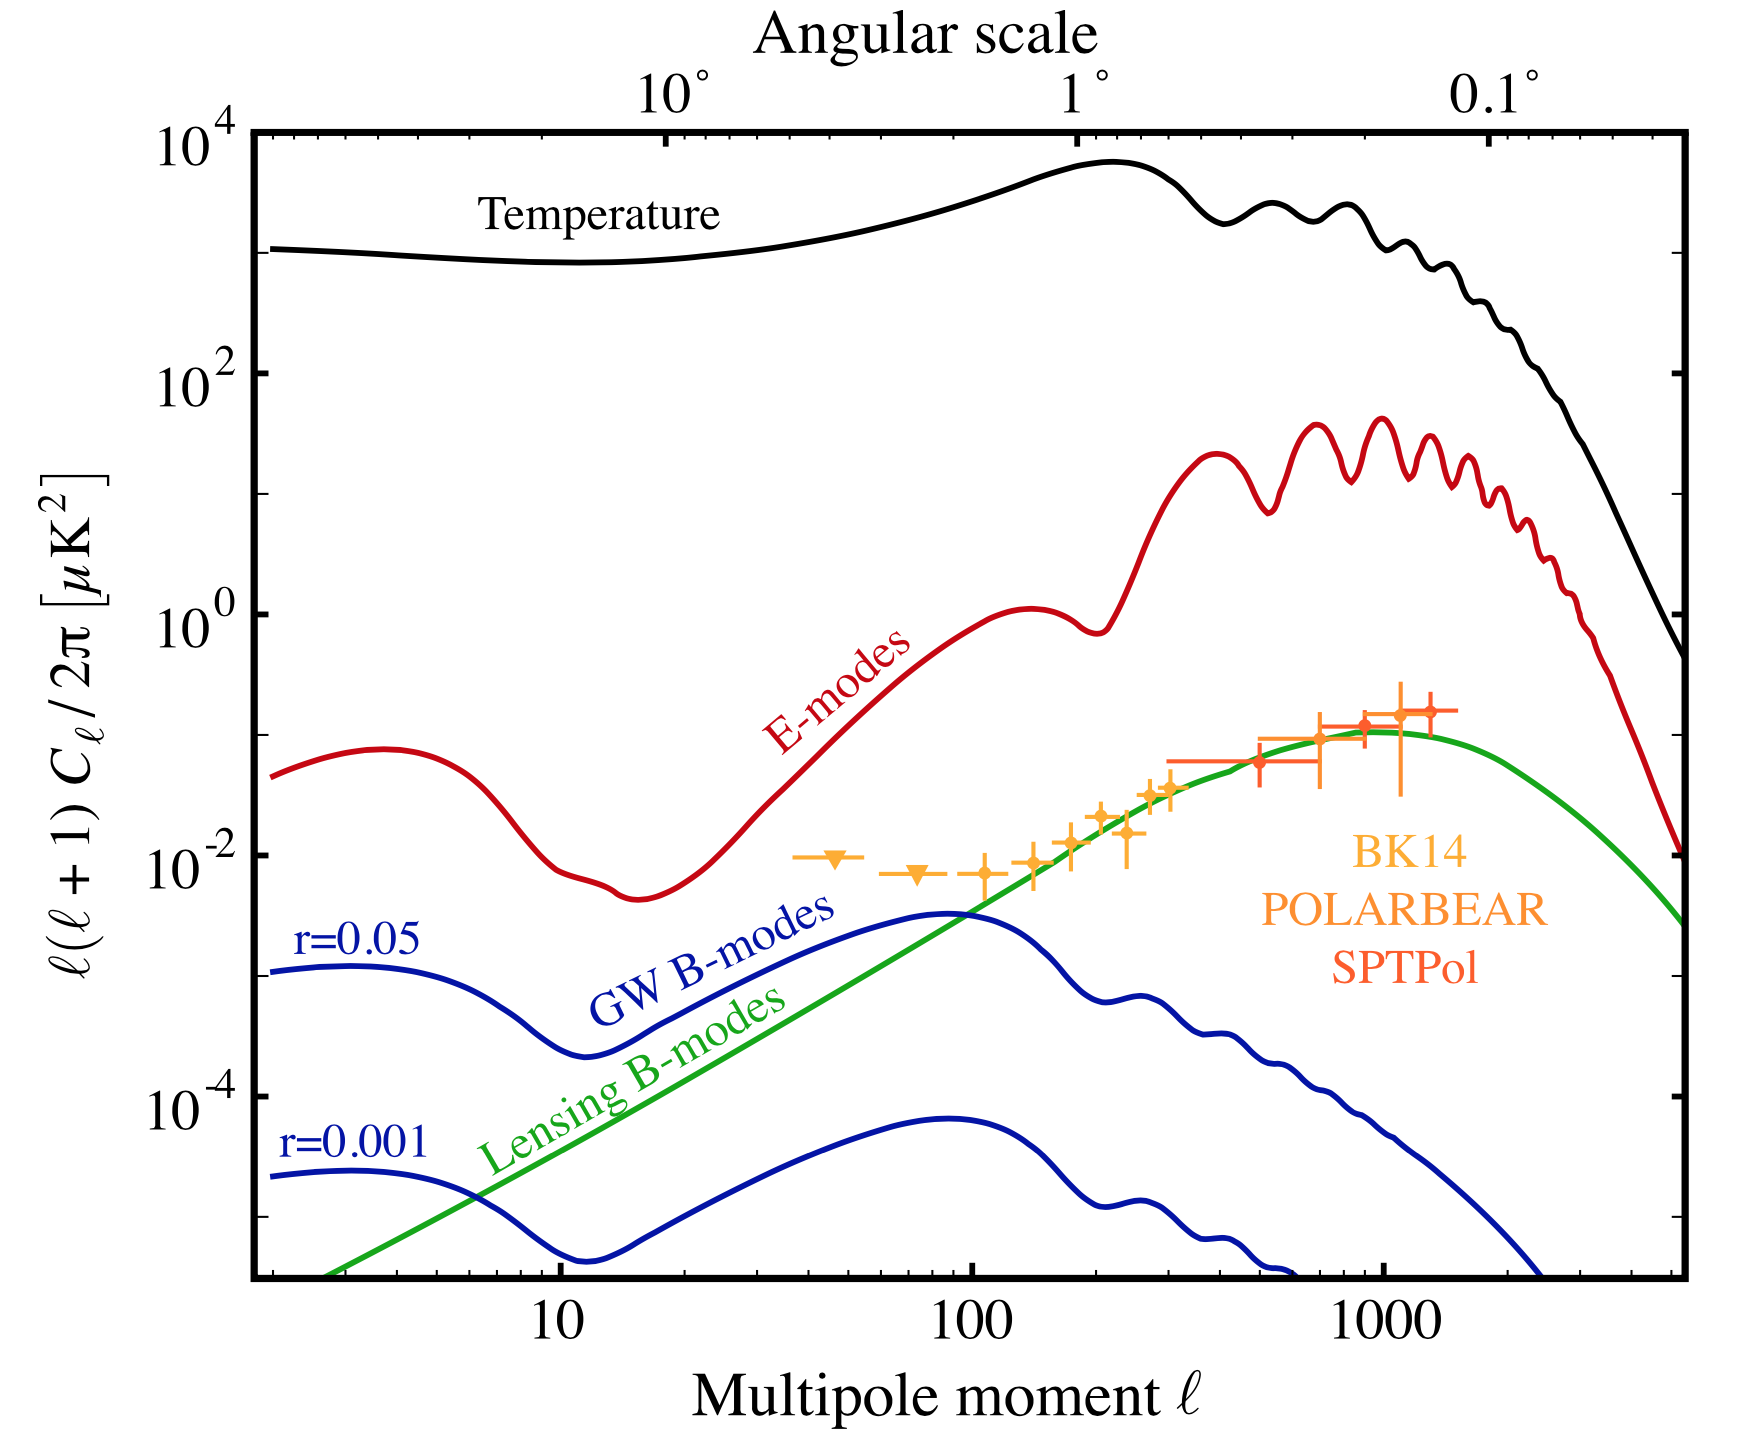
\includegraphics[width=0.7\linewidth]{../figures/power_spect.png}
	\caption{Predizioni teoriche dello spettro di potenza della temperatura (in nero), dei modi E (in rosso) e dei modi B (in blu). Lo spettro di potenza dei modi B è rappresentato per due valori diversi di \textit{r} (r=0.001 e r=0.05)\cite{libro_CMB}.}
	\label{power_spect}
\end{figure}

Se vogliamo effettuare una corretta misura della polarizzazione della CMB è necessario sottrarre al segnale misurato tutte le anisotropie dovute a oggetti presenti tra l'osservatore e la LSS. Si utilizza comunemente il termine \textit{foreground} per riferirsi a tutte le emissioni nell'intervallo di frequenze compreso tra 10 e 1000 GHz presenti tra noi e il guscio sferico definito dalla LSS.
Il problema della separazione delle componenti (\textit{component separation}) implica la necessità di effettuare misure a multibanda lungo tutto il range di frequenze comprese tra 10 e 1000 GHz con una sensibilità sufficiente per poter rivelare il debole segnale dei modi B e allo stesso tempo caratterizzare il foreground ed ottenere una mappa pulita della CMB.


    %%%%%%%%%%%%%%%%%%%  CAPITOLO 1.2  %%%%%%%%%%%%%%%%%%%
\section{Diagramma di radiazione}\label{rad_pattern}
Un sistema ottico è un dispositivo il cui scopo è quello di focalizzare la luce proveniente dal cielo e farla propagare verso un rivelatore.


Per l'analisi della CMB è nostro interesse studiare la direzione di provenienza della radiazione. Consideriamo quindi, d'ora in poi, un fascio d'antenna modellato per misurare il segnale che proviene da una direzione specifica.
La risposta di un sistema ottico ideale può essere allora rappresentata come una delta di Dirac: non nulla solo lungo la linea di vista.
Tuttavia i fenomeni di interferenza e diffrazione rendono la situazione molto più complessa; in particolare nella radio astronomia e nell'astronomia a microonde il problema è particolarmente importante poiché le dimensioni degli elementi ottici degli strumenti sono comparabili con le lunghezze d'onda d'interesse.


La risposta angolare di un sistema ottico è quantificata da una funzione $\gamma(\theta,\phi)$ detta \textit{beam function} che definisce il \textbf{diagramma di radiazione}. Idealmente $\gamma(\theta,\phi)$ dovrebbe corrispondere a una delta di Dirac\footnote{Questa idealizzazione viene spesso chiamata \textit{pencil beam idealization}} ma quello che viene in realtà osservato è una risposta simile a quella riportata in Fig.~\ref{diag_rad}.
\`E possibile osservare la presenza di un \textit{main beam} e di lobi secondari. Tipicamente la maggior parte della radiazione è contenuta nel main beam.
\begin{figure}[!ht]
\centering
	\begin{subfigure}{0.5\textwidth}
	    \centering
	    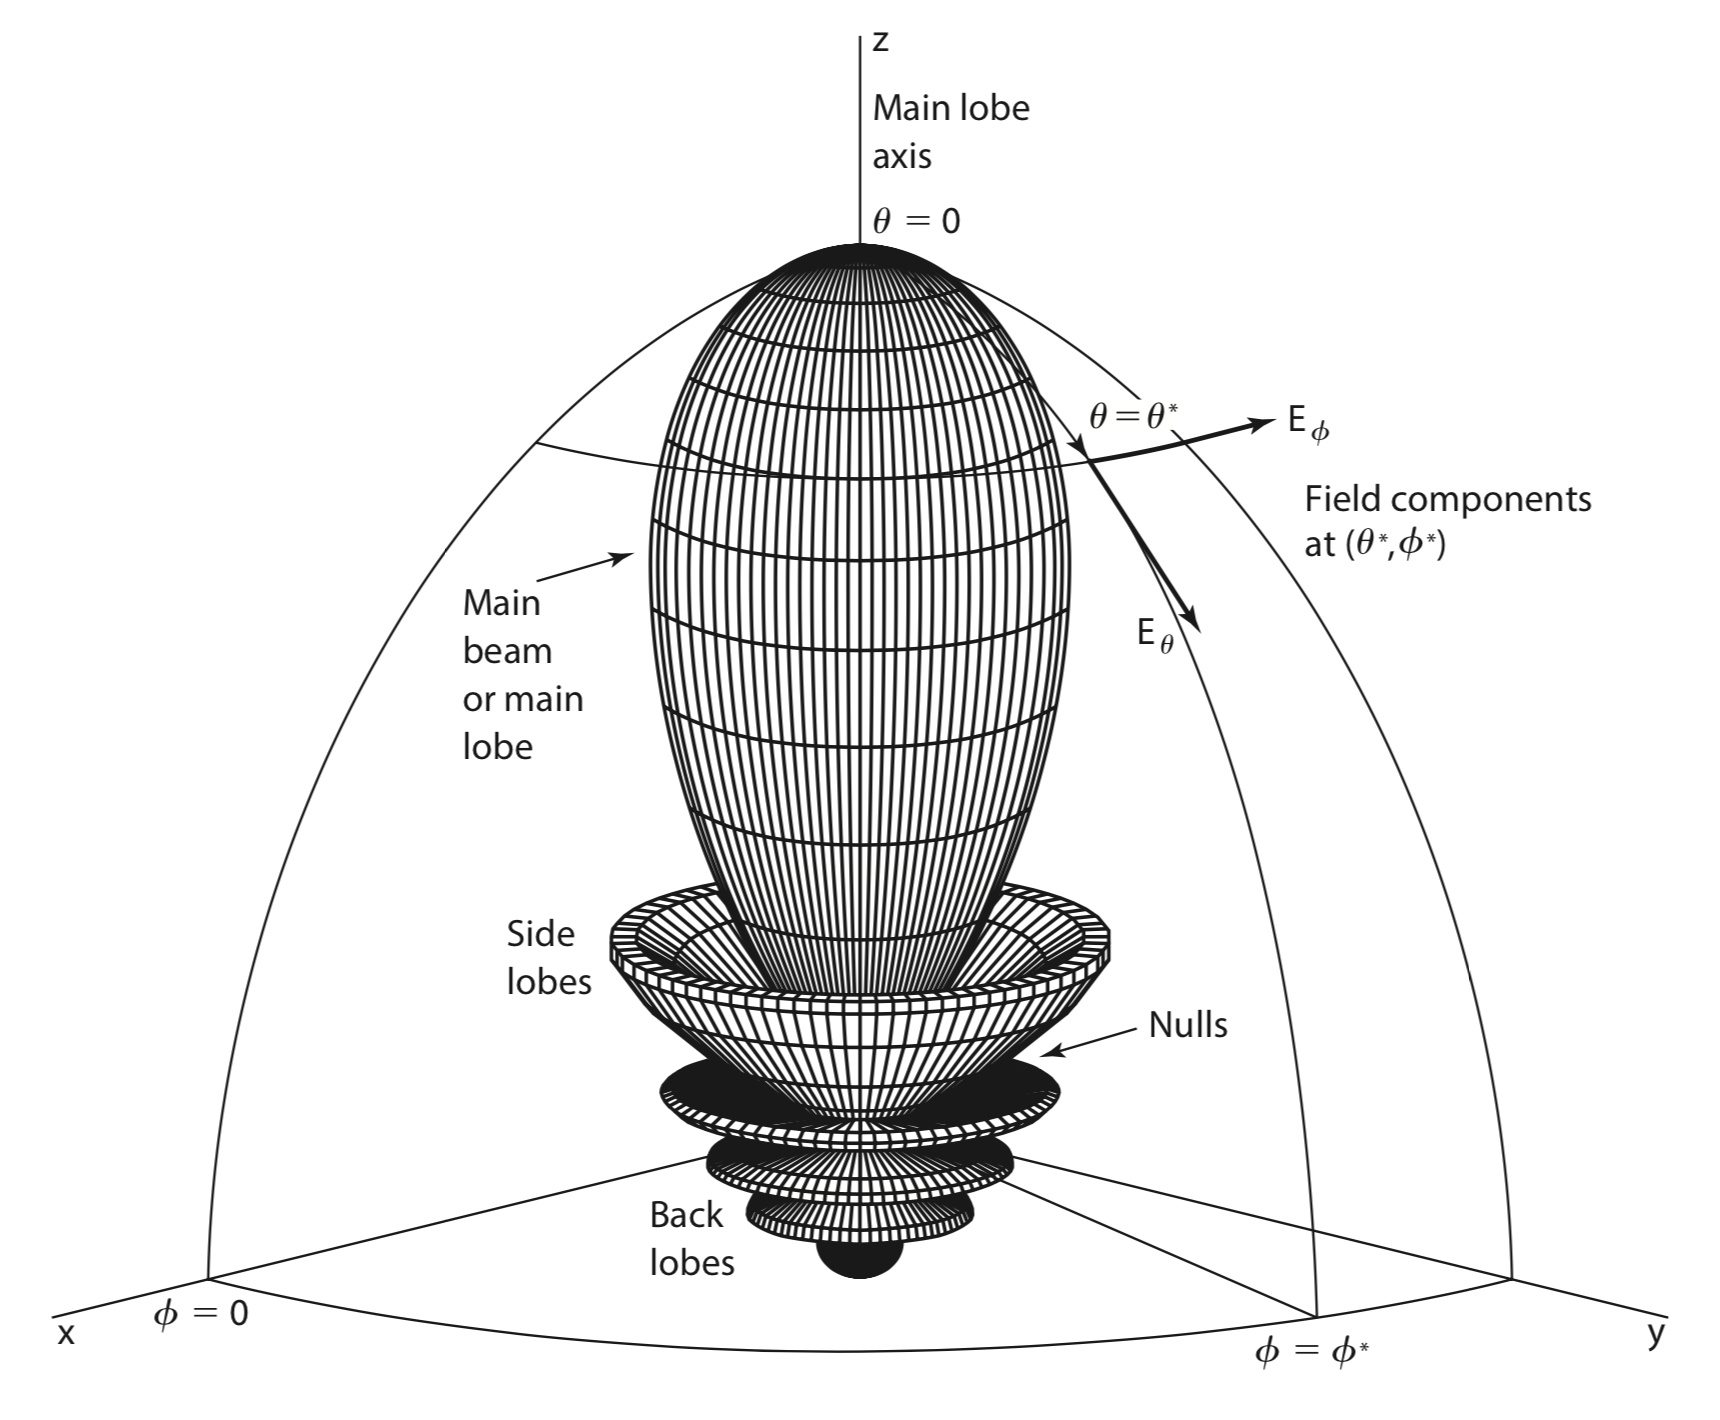
\includegraphics[width=\linewidth]{../figures/diag_rad}
	    \caption{}
	    \label{beam}
	\end{subfigure}
	\begin{subfigure}{0.45\textwidth}
		\centering
	    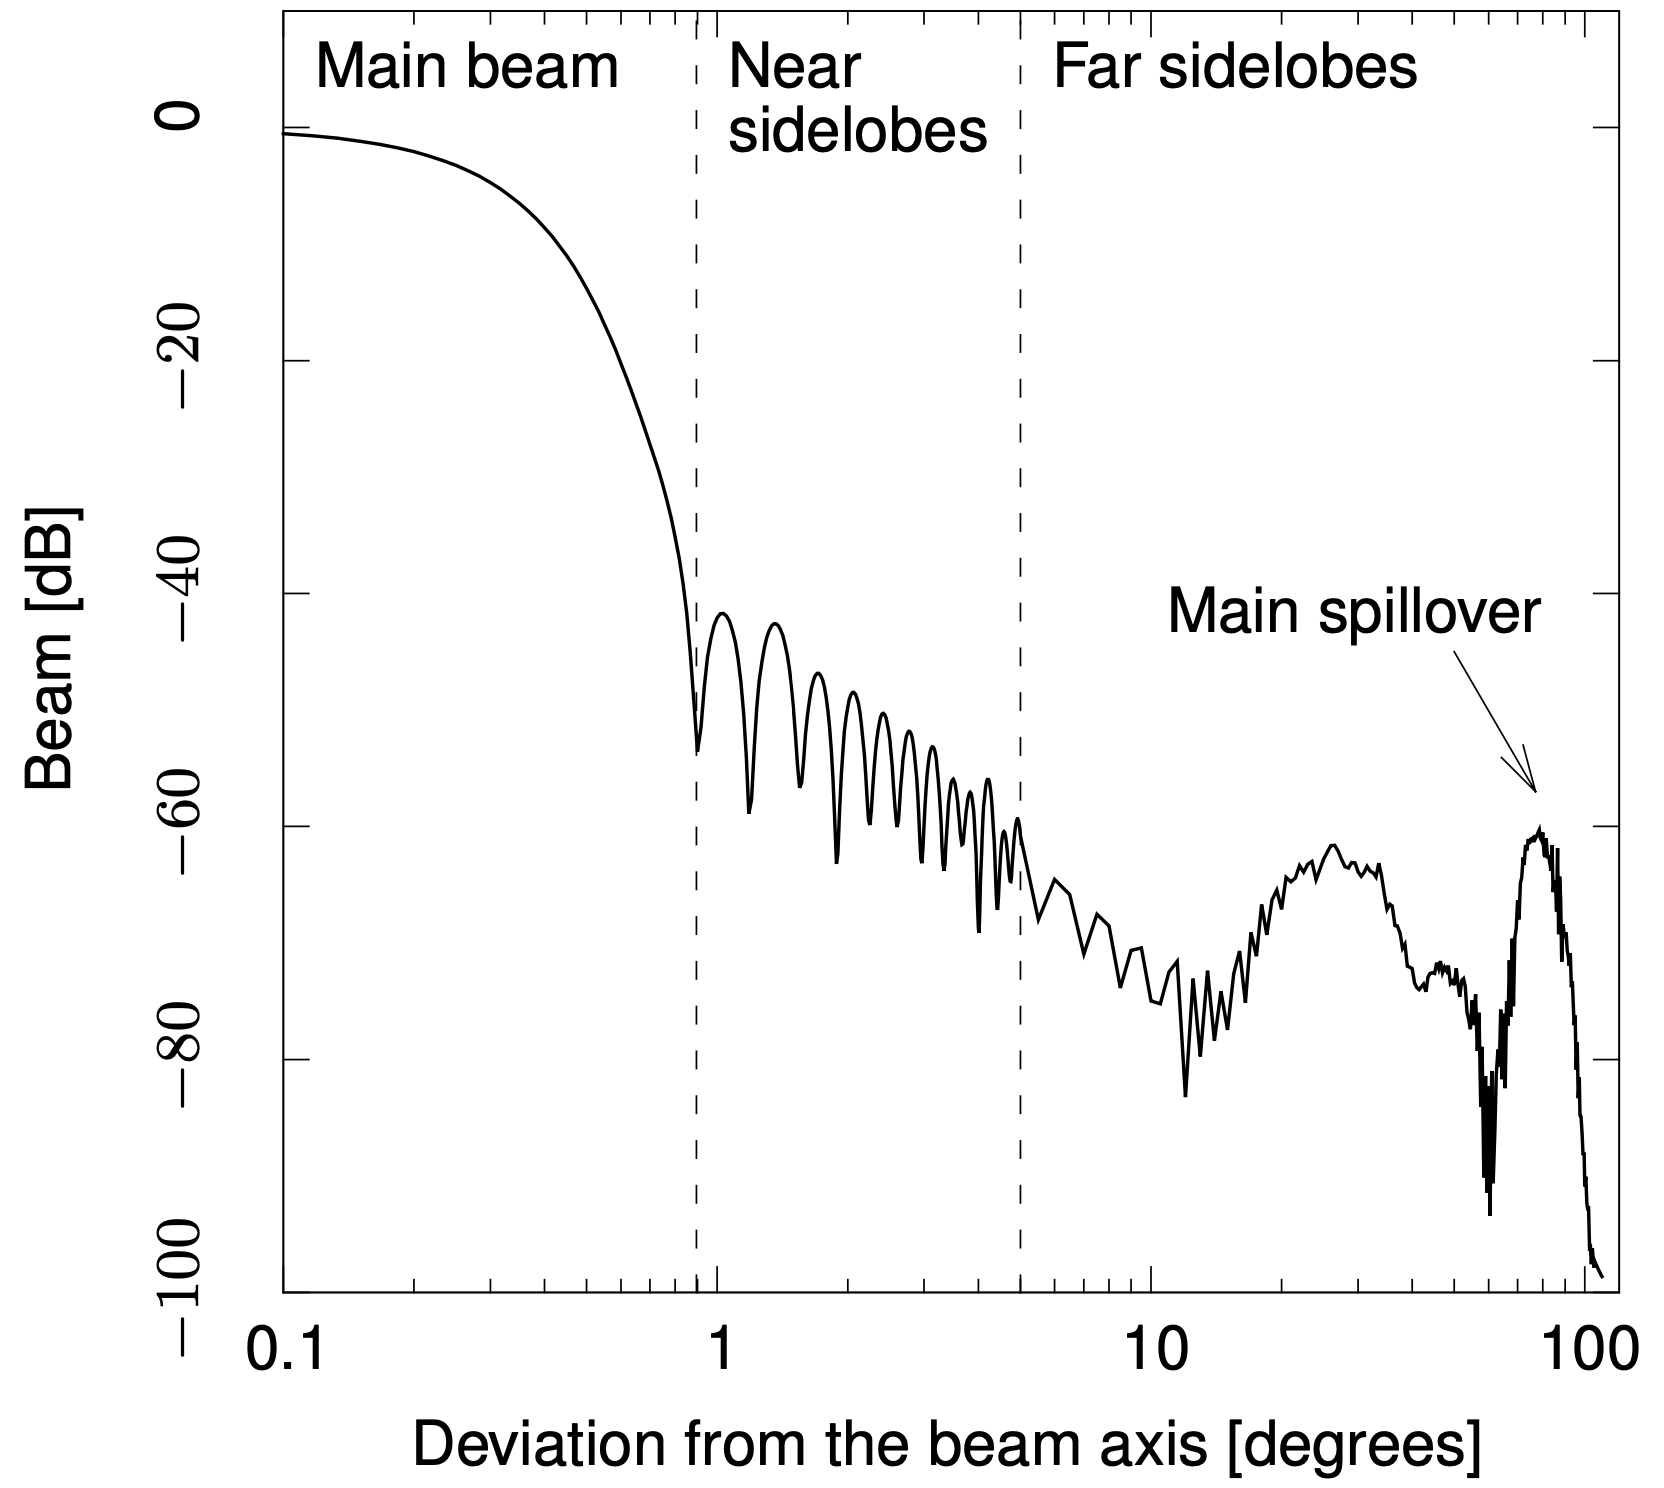
\includegraphics[width=\linewidth]{../figures/risposta_ottica.png}
		\caption{}
		\label{beam_cut}
	\end{subfigure}
\caption{Tipico andamento della \textit{beam function} $\gamma(\theta,\phi)$. La Fig.~\ref{beam} rappresenta il diagramma di radiazione tridimensionale di un'antenna direzionale.\cite{cmb}. La Fig.~\ref{beam_cut} rappresenta una sezione dello stesso grafico su un piano parallelo all'asse del main lobe.\cite{planck}}
\label{diag_rad}
\end{figure}
%%%%%
A partire dal diagramma di radiazione si definiscono alcuni parametri che permettono una sua descrizione; tali parametri sono i protagonisti di questo lavoro di tesi.
La \textbf{Full Width Half Maximum} (FWHM) (Fig.~\ref{fwhm}) del main beam è la larghezza angolare a metà della sua altezza ed è uno dei parametri più importanti e più diffusi per la caratterizzazione della risoluzione di uno strumento\footnote{Tale parametro viene anche indicato come $\theta_\text{FWHM}$}. Nel corso dei prossimi capitoli verranno considerati due diversi valori per la FWHM, rispetto all'asse $x$ e rispetto all'asse $y$. Attraverso queste due grandezze è possibile definire un ulteriore parametro: l'\textbf{ellitticità}. Questa è definita come il rapporto tra le due FWHM ponendo al numeratore la più grande tra $\text{FWHM}_\text{x}$ e $\text{FWHM}_\text{y}$.
Hanno inoltre grande importanza i parametri che riguardano la polarizzazione. Supponiamo di studiare un'antenna in trasmissione\footnote{Strumenti ottici per lo studio della CMB lavorano in ricezione ma è possibile studiare alternativamente un'antenna in trasmissione per il \textit{principio di reciprocità}.} e considerare un segnale polarizzato linearmente lungo una determinata direzione.
\`E possibile definire una componente \textit{co-polare} ed una componente \textit{cross-polare} della radiazione (Fig.~\ref{plane_cut}). La componente co-polare è la frazione radiazione irradiata lungo la direzione originale di polarizzazione mentre la componente cross-polare è la frazione di radiazione irradiata lungo la direzione perpendicolare a quella originale.
In particolare i parametri utilizzati nei prossimi capitoli riguardano la componente \textbf{co-polare massima} e la componente \textbf{cross-polare massima}. Data un'antenna in polarizzazione lineare il piano su cui giace il campo elettrico dell'onda trasmessa (o ricevuta) è detto piano E, mentre il piano ad esso perpendicolare è detto piano H.

\begin{figure}[!ht]
	\centering
	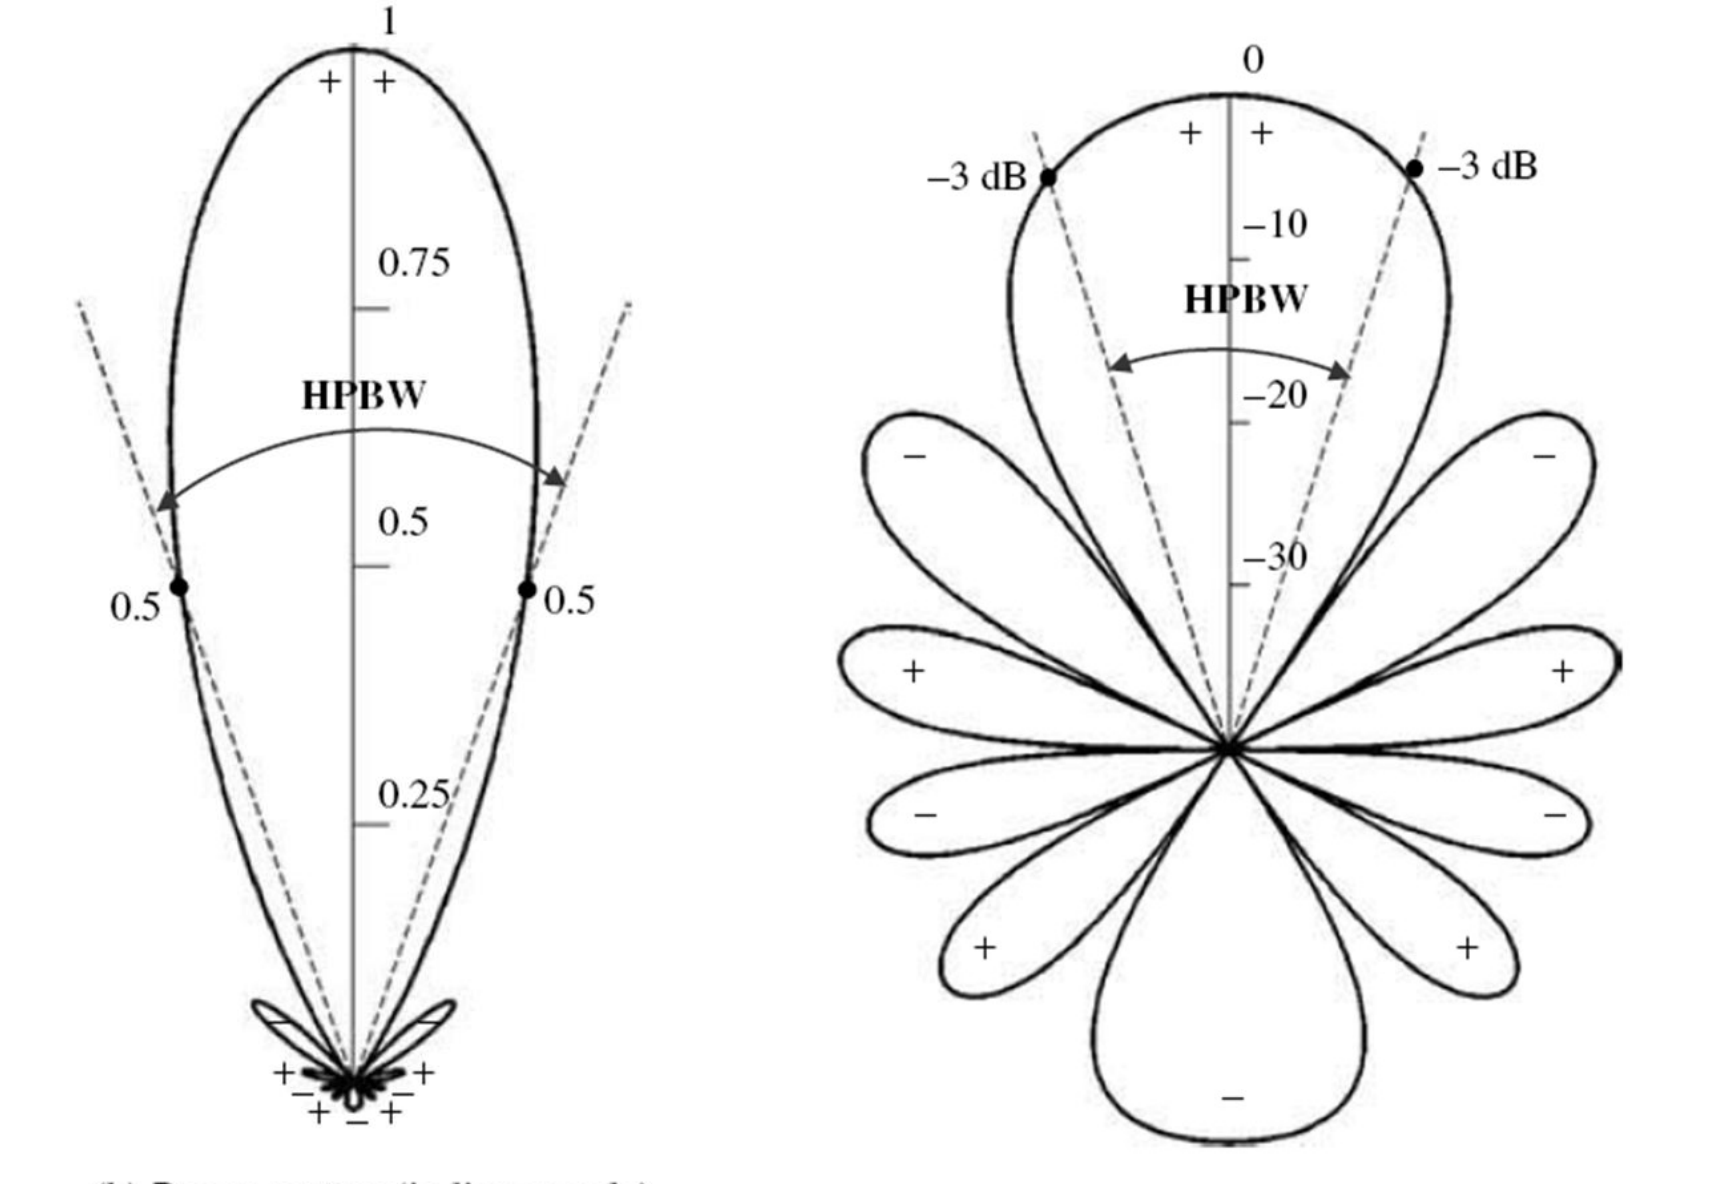
\includegraphics[width=0.8\linewidth]{../figures/fwhm.png}
	\caption{Rappresentazione schematica che mostra la FWHM. HPBW (Half Power Beam Width) e FWHM rappresentano lo stesso parametro. Sulla sinistra è rappresentata una beam function in scala lineare mentre sulla destra in scala logaritmica, la metà altezza del fascio si trova a $-3 \unit{dB}$ rispetto al massimo.}
	\label{fwhm}
\end{figure}

\begin{figure}[!ht]
	\centering
	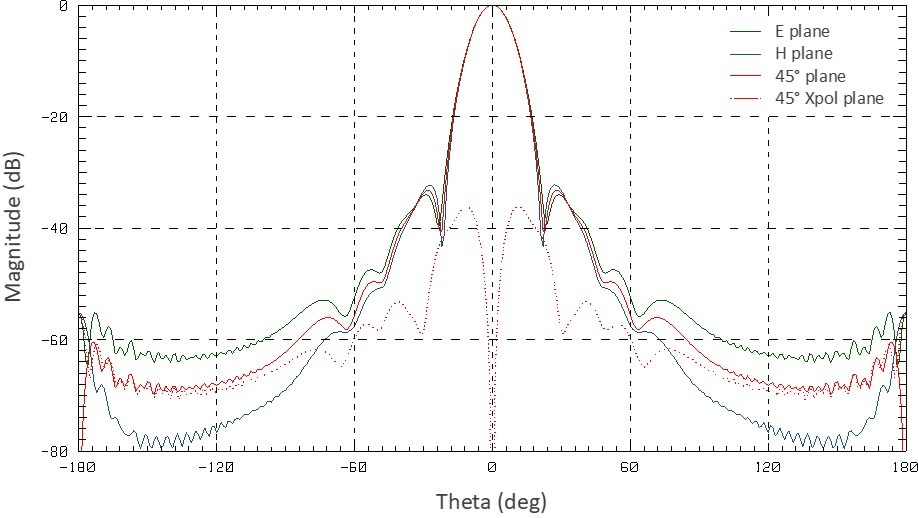
\includegraphics[width=\linewidth]{../figures/plane_cut.png}
	\caption{In questo grafico è rappresentata la componente co-polare su vari piani: piano E, piano H e piano a $45^{\circ}$ tra i due. Per quanto riguarda quest'ultimo piano è rappresentata anche la componente cross-polare. Il piano a $45^{\circ}$ è particolarmente interessante perché su di esso la componente cross-polare è molto intensa.}
	\label{plane_cut}
\end{figure}

\begin{comment}
Sarebbe bene mettere una figura o due che mostrino in maniera schematica questi parametri (FWHM, max co-pol, max x-pol, magari anche l'ellitticità ma è difficile).
\end{comment}


Per fare misurazioni di CMB è necessario richiedere alcune condizioni relative agli strumenti ottici. In riferimento alla Fig.~\ref{power_spect} si nota che una certa scala angolare mi permette di selezionare i multipoli che è possibile osservare; è quindi necessario avere una FWHM che permetta di risolvere i dettagli della CMB entro certe scale angolari. La relazione approssimata che lega il valore di $\ell$ alla FWHM è: $\ell\sim{180^{\circ}}/{\theta_\text{FWHM}}$.
Inoltre il livello dello spettro di potenza dei modi B è molto più basso di quello dei foreground e dei modi E; poiché si ha grande interesse nel misurare i modi B è necessaria una grande sensibilità strumentale. Per raggiungere elevate sensibilità è fondamentale avere a disposizione vasti piani focali che mi permettano di utilizzare un elevato numero di rivelatori.
Infine, per avere una misura pulita della CMB, è essenziale rimuovere tutti i foreground e avere quindi a disposizione misure a tante frequenze diverse, il che si traduce ancora una volta nella richiesta di un elevato numero di rivelatori.



    %%%%%%%%%%%%%%%%%%  CAPITOLO 1.3  %%%%%%%%%%%%%%%%%%%%

\section{Simulazione di sistemi ottici}\label{simulazioni}
Simulare un sistema ottico significa studiare quanta potenza viene ricevuta in funzione dell'angolo rispetto alla linea di vista. 
Esistono diversi software in grado di simulare un fascio d'antenna e quindi la sua risposta angolare.

\begin{figure}[!ht]
	\centering
	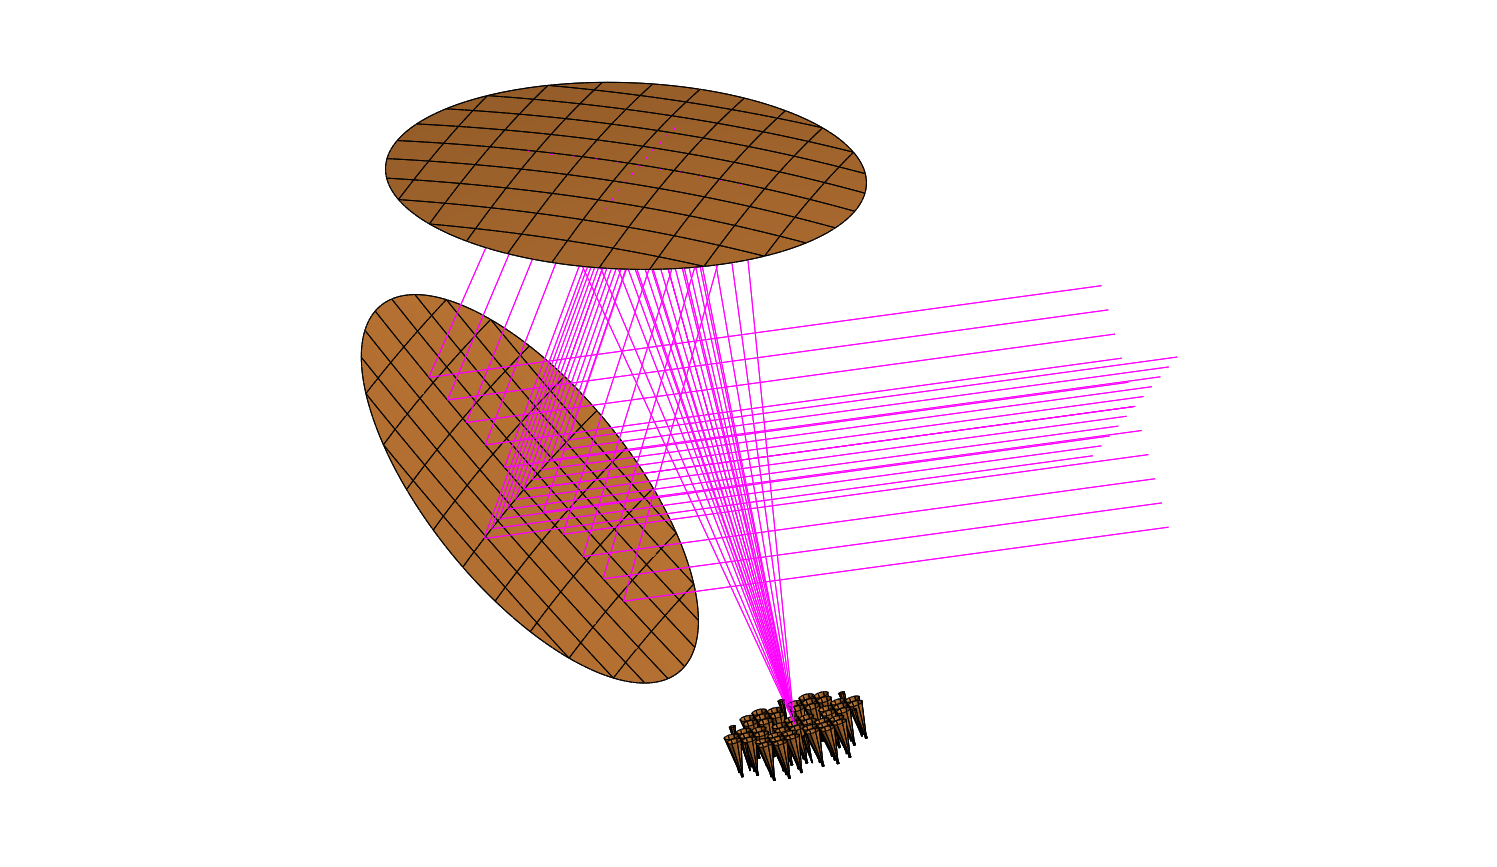
\includegraphics[width=0.6\linewidth]{../figures/strip.png}
	\caption{Modello in GRASP del telescopio di STRIP.}
	\label{strip}
\end{figure}

Nel corso di questo lavoro di tesi ho utilizzato dei dati relativi ad un particolare strumento per l'analisi della CMB: \textit{STRIP}.
Lo strumento STRIP (STRatospheric Italian Polarimeter) fa parte dell'esperimento internazionele \textit{LSPE} (Large-Scale Polarization Explorer) ideato per effettuare misure di CMB ad elevate scale angolari.
In particolare STRIP è stato progettato per la misura di radiazione a basse frequenze; esso presenta 49 antenne a 43 GHz e 6 antenne a 90 GHz. In Fig.~\ref{strip} è rappresentato il modello di STRIP attraverso il software \textit{GRASP} (General Reflector Antenna Software Package).
Attraverso GRASP è stato possibile ottenere la tabella in Fig.~\ref{dataset} che riporta le caratteristiche del beam data una posizione $(x, y, z)$ sulla superficie focale.


GRASP è uno strumento molto potente che permette di simulare sistemi ottici complessi.
Tuttavia i tempi di calcolo di GRASP sono elevati\footnote{Per produrre i dati in Fig.~\ref{dataset} sono stati impiegati due giorni.}; per ogni simulazione, e quindi per ogni antenna, vengono costruiti dei grafici come quelli riportati in Fig.~\ref{beam_grasp} e poi da quelli vengono ricavati i valori riportati nel dataset ~\ref{dataset}.
Un grafico come quello in Fig.~\ref{beam_grasp} produce quindi una singola riga della tabella ~\ref{dataset}.

\begin{figure}[!ht]
	\centering
	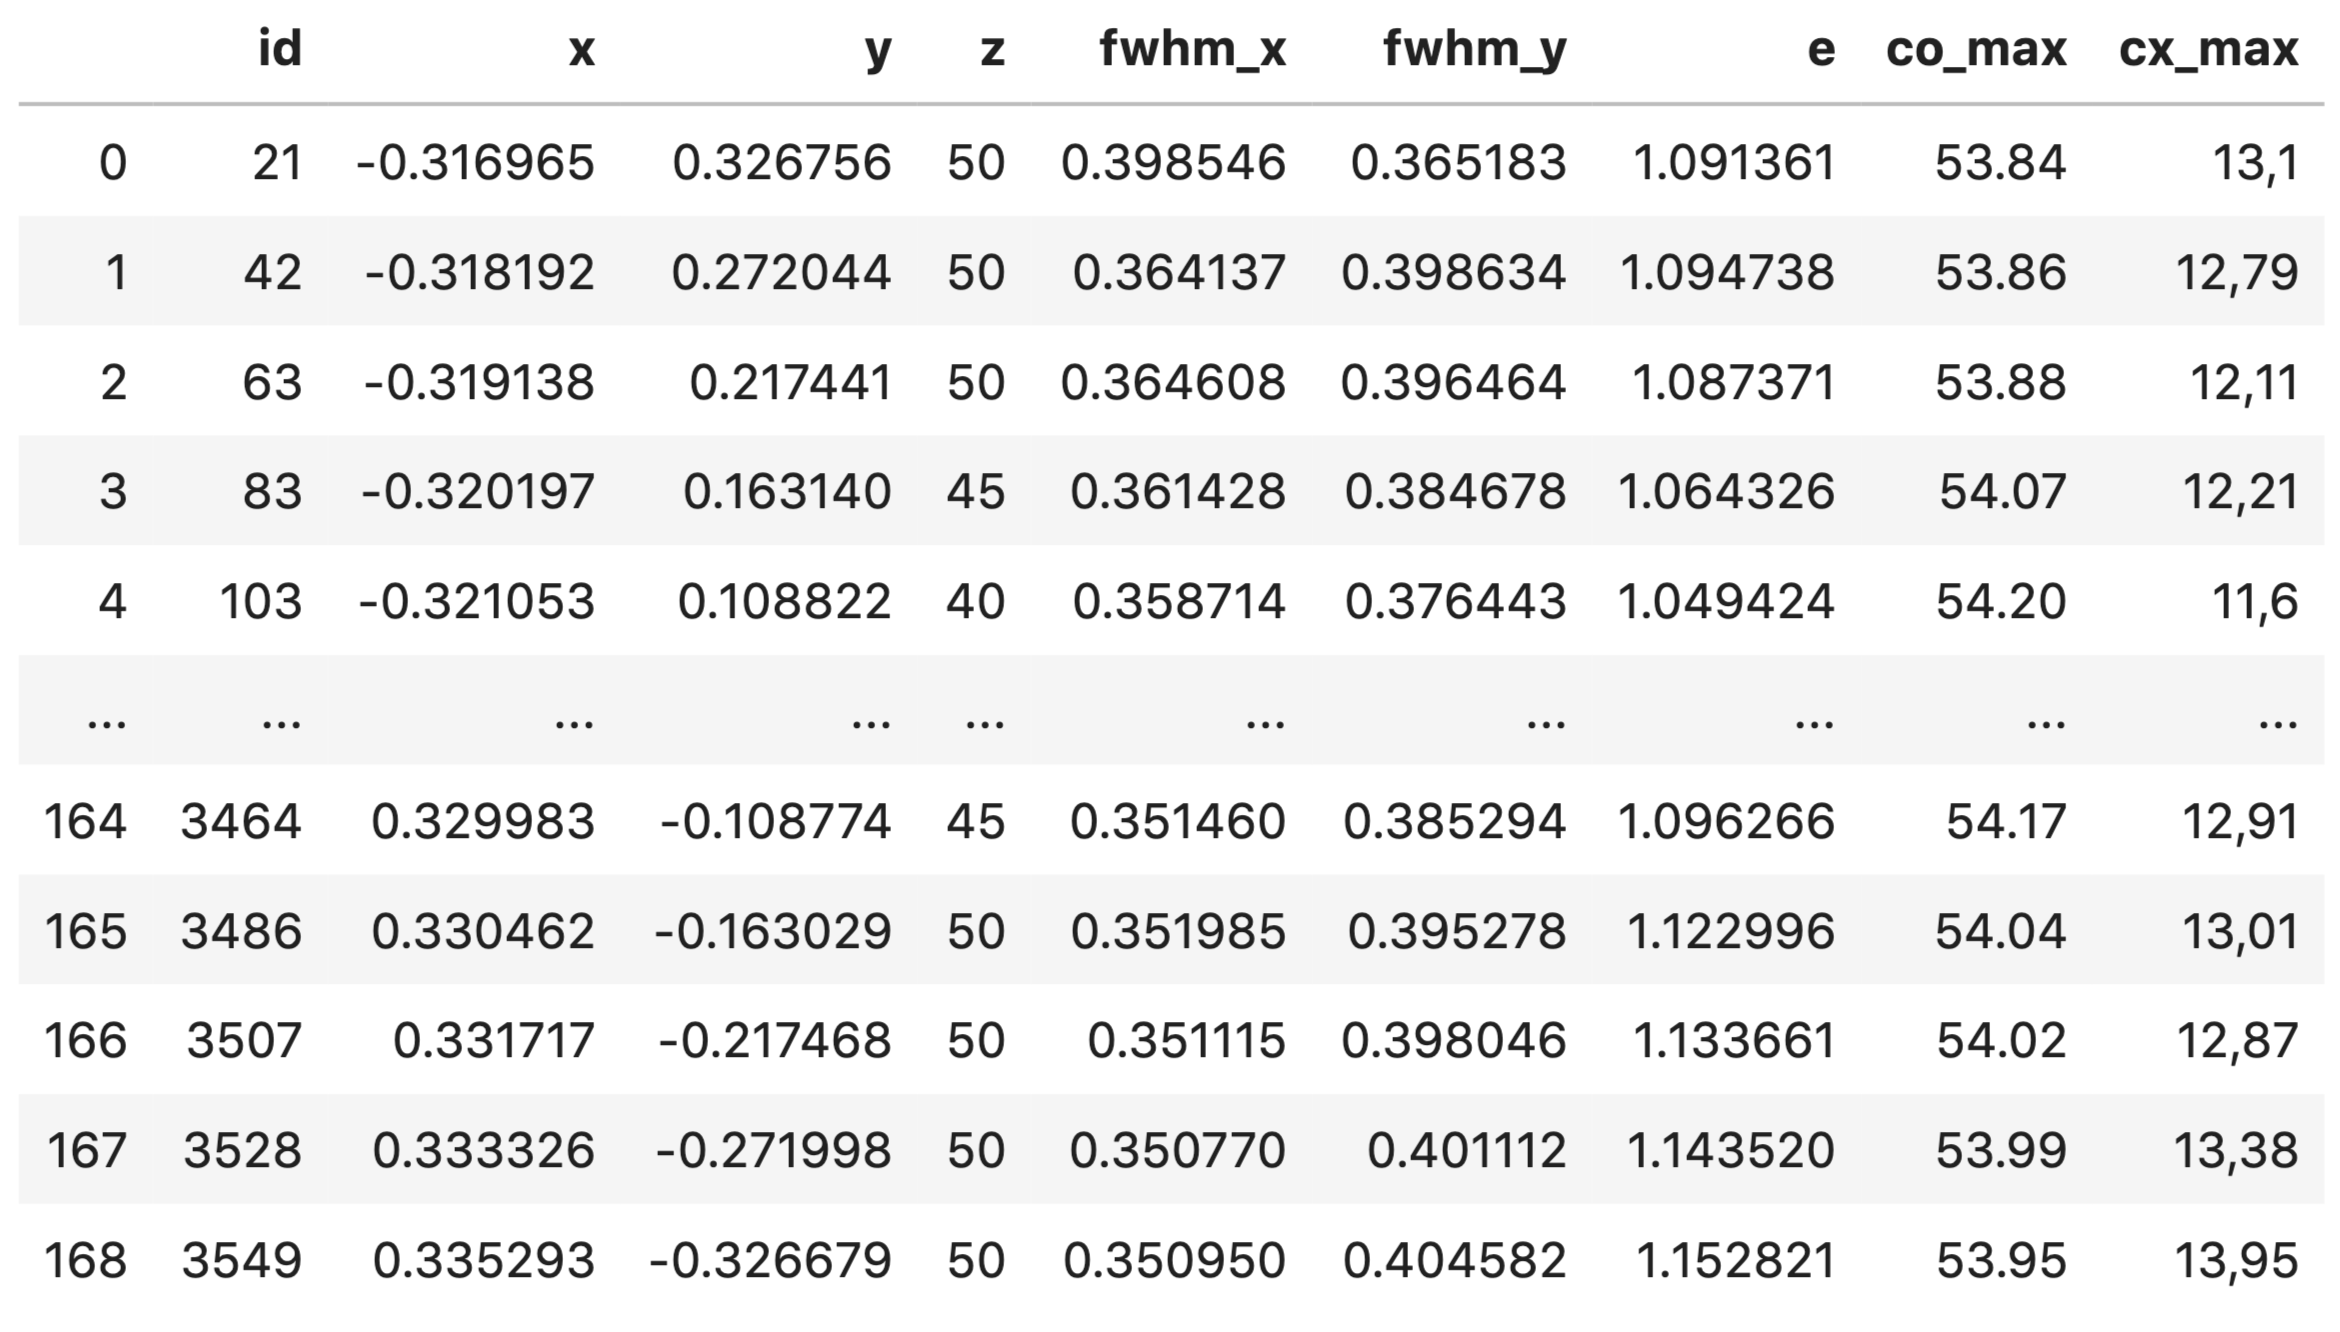
\includegraphics[width=0.8\linewidth]{../figures/dataset.png}
	\caption{Dataset relativo allo strumento STRIP ottenuto tramite la simulazione in GRASP. Tale dataset è stato utilizzato per l'analisi descritta nei capitoli successivi.}
	\label{dataset}
\end{figure}

Nel caso di STRIP è ancora possibile simulare l'intera ottica tramite GRASP poiché il numero di antenne è piuttosto limitato. Tuttavia per sistemi ottici più complessi in cui il numero di antenne diventa di circa 2 ordini di grandezza superiore, risulta del tutto impossibile effettuare una simulazione completa dell'intera ottica.
\`E quindi forte la necessità di trovare una via alternativa che permetta di stimare i parametri che descrivono il beam in una qualsiasi posizione.

\begin{figure}[!ht]
\centering
	\begin{subfigure}{0.49\textwidth}
	    \centering
	    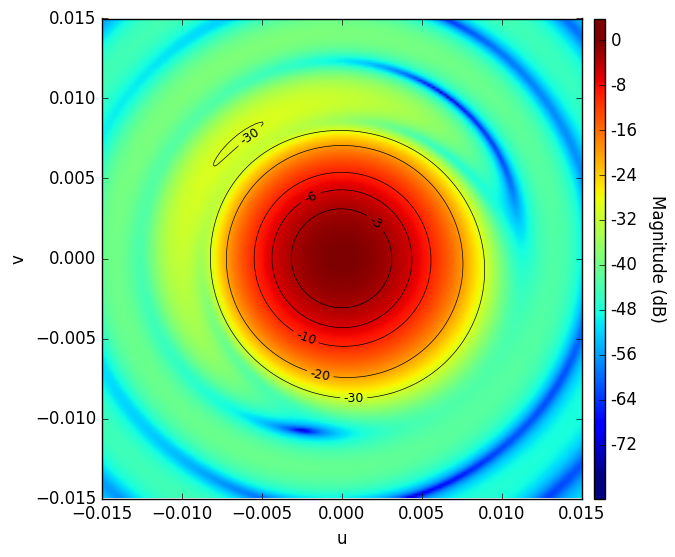
\includegraphics[width=\linewidth]{../figures/off-axis_co.png}
	    \caption{}
	    \label{off_axis_co}
	\end{subfigure}
	\begin{subfigure}{0.49\textwidth}
		\centering
	    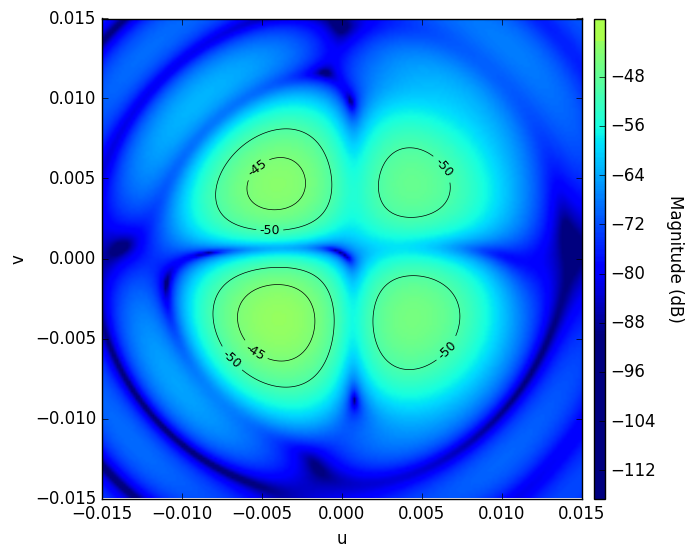
\includegraphics[width=\linewidth]{../figures/off-axis_cx.png}
		\caption{}
		\label{off_axis_cx}
	\end{subfigure}
\caption{Diagramma della componente co-polare~\ref{off_axis_co} e della componente cross-polare~\ref{off_axis_cx} di un'antenna off-axis. \`E possibile notare come il profilo del beam sia leggermente ellittico; per il sistema ottico di STRIP infatti l'ellitticità del fascio aumenta spostandosi dal centro del piano focale.}
\label{beam_grasp}
\end{figure}


%%%%%%%%%%%%%%%%%%%%%%%%%%%%%%%%%%%%%%%%%%%%%%%%%%%%%%%
%%%%%%%%%%%%%%%%%%%%%%%%%%%%%%%%%%%%%%%%%%%%%%%%%%%%%%%
%%%%%%%%%%%%%%%%%%%%%%%%%%%%%%%%%%%%%%%%%%%%%%%%%%%%%%%
%                   FINE CAPITOLO 1                   %
%%%%%%%%%%%%%%%%%%%%%%%%%%%%%%%%%%%%%%%%%%%%%%%%%%%%%%%
%%%%%%%%%%%%%%%%%%%%%%%%%%%%%%%%%%%%%%%%%%%%%%%%%%%%%%%
%%%%%%%%%%%%%%%%%%%%%%%%%%%%%%%%%%%%%%%%%%%%%%%%%%%%%%%


%%%%%%%%%%%%%%%%%%%%  CAPITOLO 2  %%%%%%%%%%%%%%%%%%%%

\chapter{Regressione con reti neurali}\label{reg_nn}

	%%%%%%%%%%%%%%%%%%%  CAPITOLO 2.1  %%%%%%%%%%%%%%%%%%%

\section{Machine learning e tipi di rete}
Il \textit{machine learning (ML)} è un campo di ricerca a metà tra statistica, intelligenza artificiale ed informatica ed è una branca della disciplina chiamata \textit{intelligenza artificiale (AI)}. La sua applicazione riguarda ormai vastissimi campi della scienza e non solo. Sono usate tecniche di machine learning per esempio per il riconoscimento facciale o per i suggerimenti di prodotti da comprare sulle piattaforme di shopping online, ma anche in ambito medico per la diagnosi di particolari malattie.


Negli ultimi decenni il campo del machine learning si è fortemente evoluto. È stata costruita un'ampia classe di algoritmi in grado di approssimare molto efficacemente processi non lineari. Una branca del ML vede protagoniste le \textit{reti neurali artificiali (ANN)}\footnote{Spesso vengono chiamate semplicemente reti neurali (NN).}.
Queste tecniche si basano sull'apprendimento tramite esempi, i quali sono rappresentati da coppie input-output come un'immagine e la sua descrizione (input: foto di un gatto, output: "gatto") o una posizione a cui è associato un particolare valore di campo elettrico (input: (x, y, z), output: E(x, y, z)). È quindi di fondamentale importanza avere a disposizione un ampio database attraverso il quale effettuare un \textbf{training}.
Una rete neurale approssima una funzione $y=f(x)$ tramite una serie di neuroni connessi tra loro. Ogni neurone è caratterizzato da 2 parametri, come spiegato in Sez.~\ref{struttura_rete}, e l'approssimazione della relazione tra $x$ e $y$ è effettuata tramite l'ottimizzazione di tali parametri a partire dalle coppie $(x, y)$ che descrivono il comportamento della funzione $f$ in casi realistici. L'ottimizzazione dei parametri è da intendersi in termini di minimizzazione di una particolare funzione che prende il nome di \textbf{loss function}, che quantifica la discrepanza tra il comportamento di $f$ e quello della rete neurale. Riassumendo, quello che accade all'interno di una rete neurale quando si vuole approssimare una corrispondenza tra input e output è una modifica dei parametri di rete in modo da ottenere un valore di \textit{loss} il più piccolo possibile. 


Il \textit{deep learning} è un'ulteriore branca delle NN che entra in gioco quando si utilizzano reti neurali con un elevato numero di layers e di neuroni: le \textit{deep neural networks}. In questo lavoro di tesi ho creato reti con un ridotto numero di layers, queste non rientrano nel campo del deep learning.


Esistono due classi di problemi affrontati con la tecnica delle reti neurali: la \textit{classificazione} e la \textit{regressione}.
Si ha una rete classificazionale se nell'approssimare $y=f(x)$, $y$ può assumere un valore preso dagli elementi di un insieme discreto, mentre si ha una rete regressionale quando $y$ può assumere un continuo di valori.
La classificazione individua l'appartenenza ad una classe e può essere supervisionata o non supervisionata. Parliamo di classificazione supervisionata quando sono note a priori le diverse classi di appartenenza; se invece si vogliono determinare delle classi di similitudine senza conoscere a priori i pattern rappresentativi, si ha un problema di classificazione non supervisionata.
Un esempio di classificazione supervisionata è il riconoscimento di un numero a partire da un'immagine manoscritta. Un esempio invece di classificazione non supervisionata si ha quando, a partire da immagini di cifre manoscritte, si vuole determinare quali tra esse rappresentino lo stesso numero.


Le reti neurali per la regressione entrano in gioco quando, date delle coppie input-output, si vuole determinare la funzione che approssimi al meglio la relazione. Per effettuare la stima delle proprietà di un diagramma di radiazione (Sez.~\ref{reti_neurali}) ho utilizzato quest'ultimo tipo di reti neurali. In particolare la ricerca alla base di questo lavoro di tesi è stata quella di una rete neurale che permettesse, a partire da una posizione sulla superficie focale, di stimare il valore di un determinato parametro del diagramma di radiazione. Come sarà possibile notare nei paragrafi successivi, la posizione sulla superficie focale è data da una coppia $(x, y)$, senza considerare la coordinata $z$; ho deciso di procedere così poiché i punti si trovano su una superficie ben definita, il che significa che dati $x$ e $y$ la $z$ è univocamente determinata.


Il programma utilizzato in questa tesi per sviluppare i codici che permettono di effettuare questo task è Python. Questo fornisce librerie apposite per il caricamento, l'analisi e la visualizzazione dei dati; le librerie utilizzate nei codici implementati sono: \textit{pandas}, \textit{numpy}, \textit{matplotlib}, \textit{seaborn}, \textit{pytorch}.

	%%%%%%%%%%%%%%%%%%%  CAPITOLO 2.2  %%%%%%%%%%%%%%%%%%%

\section{Struttura di una rete neurale}\label{struttura_rete}
Unarete neurale è basata sull'interconnessioni di unità fondamentali: i \textbf{neuroni}.
Essa può essere rappresentata come in figura~\ref{schema_rete}.
\begin{figure}[!ht]
	\centering
	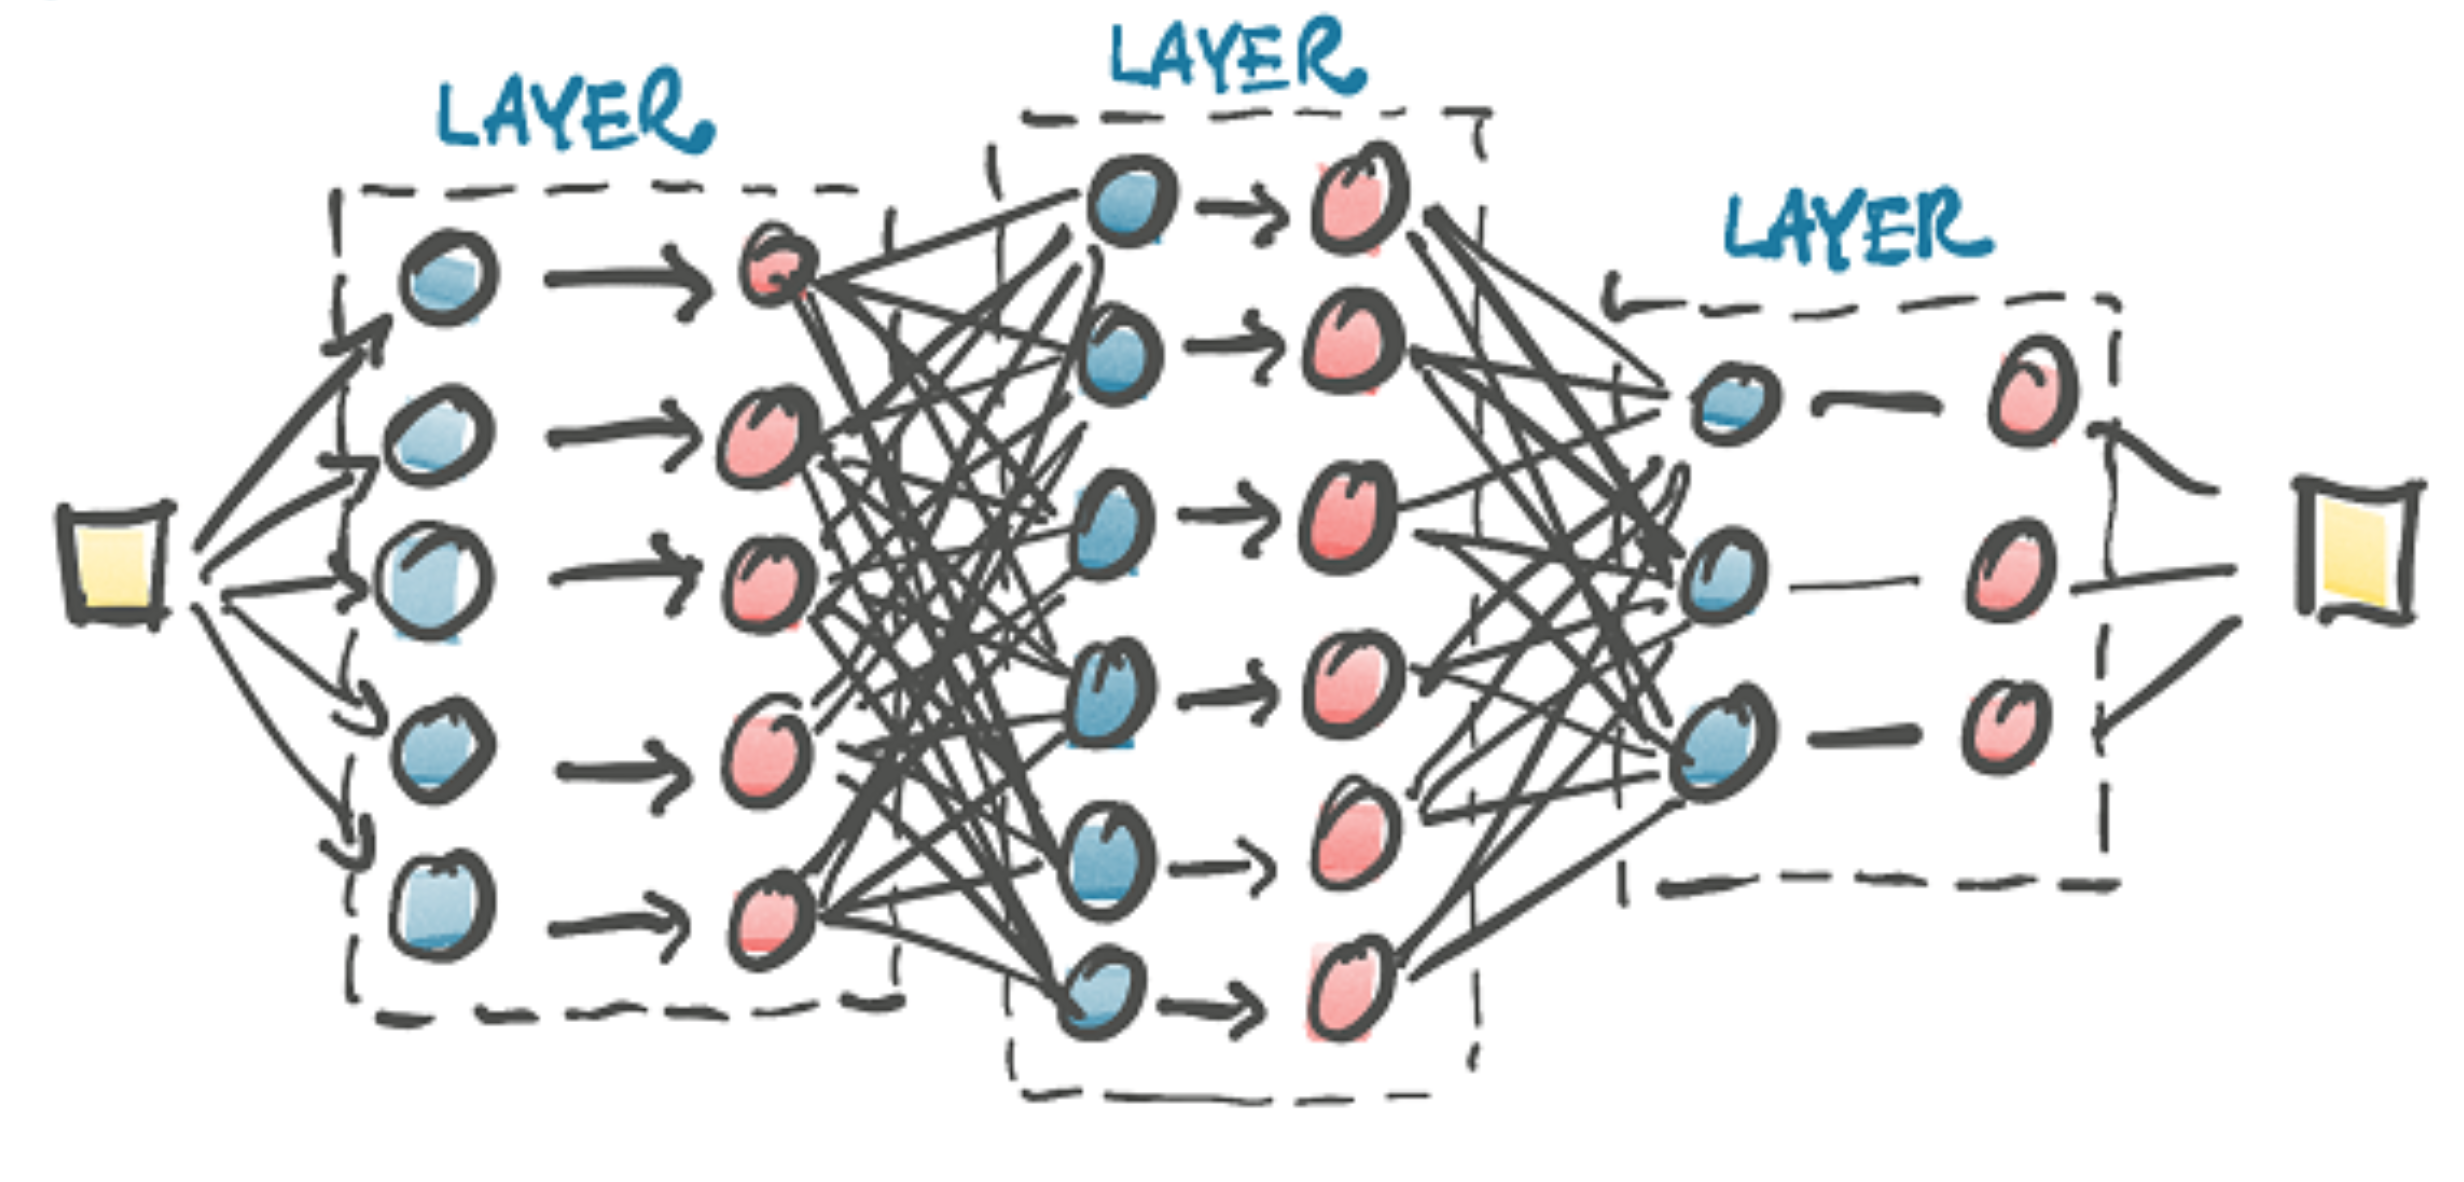
\includegraphics[width=0.6\linewidth]{../figures/schema_rete.png}
	\caption{Schema di una rete neurale con tre hidden layers. Il quadrato giallo sulla sinistra rappresenta l'input layer mentre quello sulla destra rappresenta l'output layer. Immagine presa da \textit{Deep Learning with PyTorch}, E. Stevens, L. Antiga\cite{stevens}.}
	\label{schema_rete}
\end{figure}
Un insieme di neuroni che agiscono allo stesso livello è detto \textbf{layer} e l'interconnessione di diversi layers forma una rete.
Un neurone è rappresentato da una funzione non lineare, detta \textbf{funzione di attivazione}, applicata ad una trasformazione lineare. Ogni neurone è caratterizzato da due parametri liberi: \textit{w (weight)} e \textit{b (bias)}. L'espressione matematica che descrive un singolo neutrone è quindi:
\[o=f(wx+b)\]
 dove $x$ è il dato di input, $o$ rappresenta l'output e $f$ una determinata funzione di attivazione non lineare.

\begin{figure}[!ht]
	\centering
	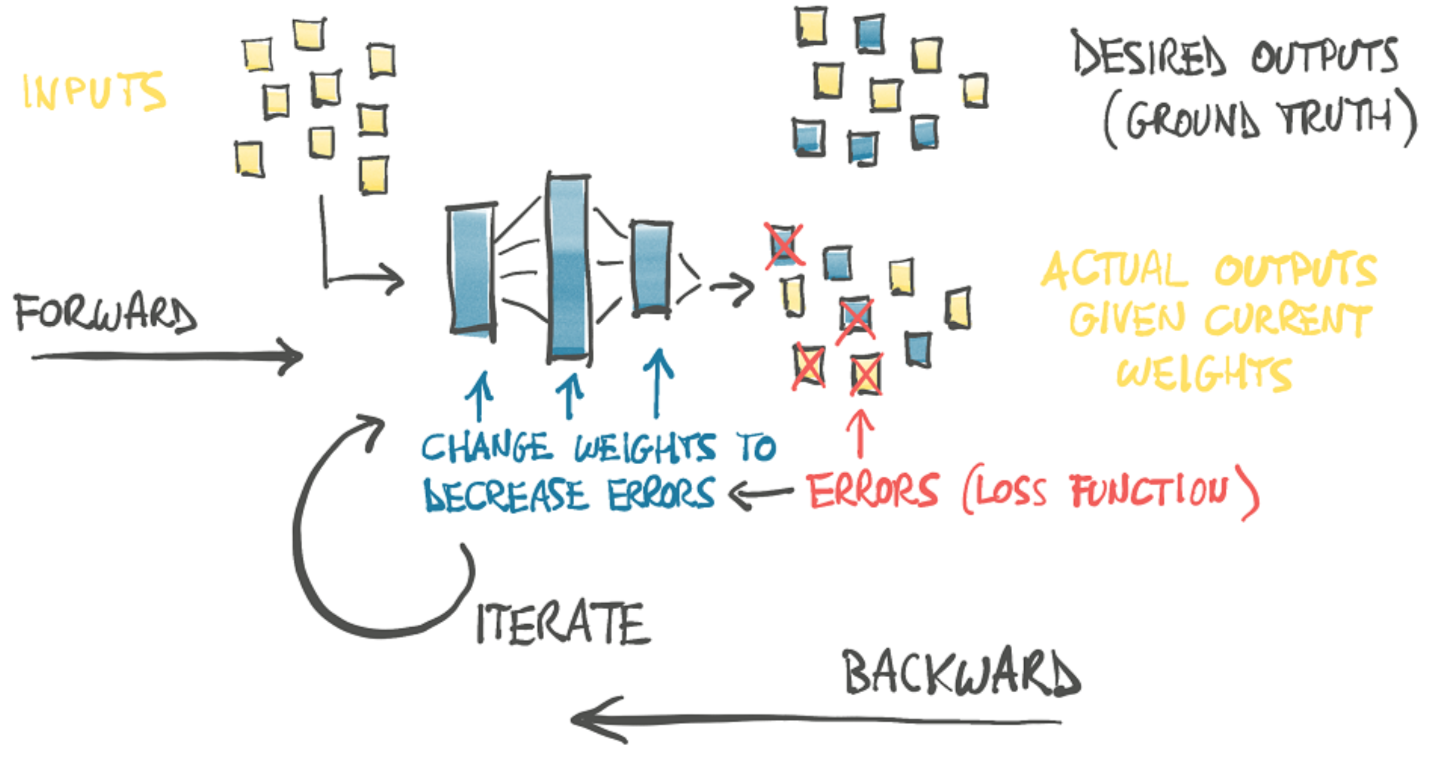
\includegraphics[width=0.7\linewidth]{../figures/learning_process.png}
	\caption{Schema del processo di apprendimento di una rete neurale. Immagine presa da \textit{Deep Learning with PyTorch}, E. Stevens, L. Antiga\cite{stevens}.}
	\label{apprendimento}
\end{figure}

Il cuore del processo di apprendimento, mostrato schematicamente in Fig.~\ref{apprendimento}, sta nella stima dei giusti parametri (weights e biases) della rete. Questo avviene seguendo determinati step:
\begin{itemize}
	\item vengono forniti alla rete inputs e outputs desiderati;
	\item il modello calcola gli outputs a partire dagli inputs forniti; questo step prende il nome di \textit{forward pass}; 
	\item viene misurato l'errore comparando l'output calcolato e quello fornito in partenza. La funzione che quantifica tale discrepanza è detta \textit{loss function};
	\item vengono modificati i parametri di rete in modo da minimizzare la loss function; questo step prende il nome di \textit{backward pass}\footnote{Tale valutazione viene fatta da un \textit{optimizer} attraverso la valutazione del gradiente dell'errore rispetto ai parametri di rete.};
	\item viene ripetuta l'intera procedura fino alla convergenza della rete, ovvero fino a che la loss function non raggiunge un andamento stabile.
\end{itemize}

\begin{figure}[!ht]
	\centering
	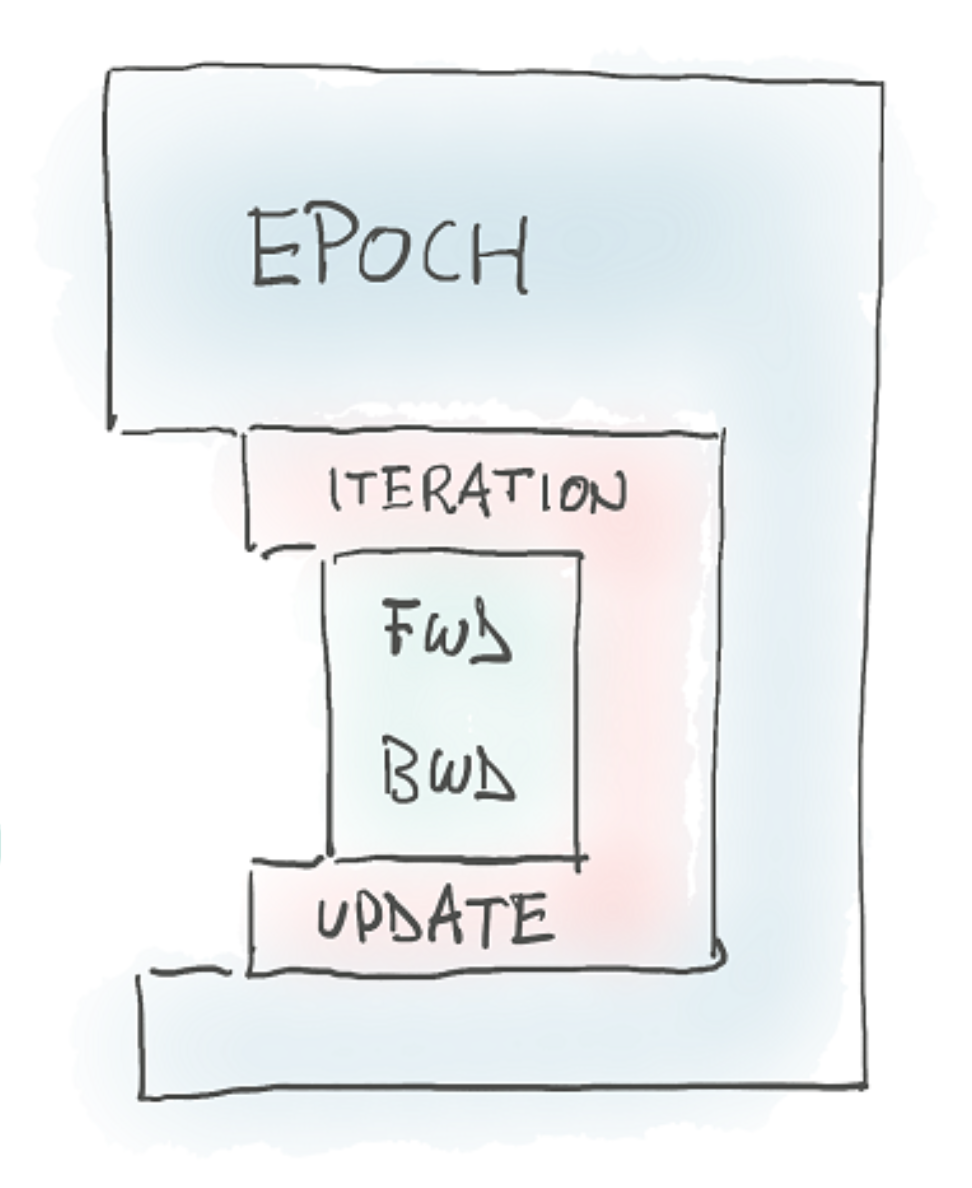
\includegraphics[width=0.4\linewidth]{../figures/ciclo_training.png}
	\caption{Rappresentazione schematica del ciclo di training. Immagine presa da \textit{Deep Learning with PyTorch}, E. Stevens, L. Antiga\cite{stevens}.}
	\label{ciclo_training}
\end{figure}

Com'è possibile notare dalla Fig.~\ref{ciclo_training}, un ciclo completo su tutti i dati messi a disposizione per l'apprendimento viene chiamato \textit{epoca}; la fase di apprendimento avviene attraverso numerose epoche.


Le reti che ho costruito, descritte in dettaglio nella Sez.~\ref{architettura}, sono chiamate \textit{reti neurali feed-forward}; il termine sta ad indicare che le connessioni tra i neuroni non formano dei cicli\footnote{Le reti che presentano cicli al loro interno vengono chiamate \textit{ricorsive}.}. In particolare si tratta di reti \textit{fully connected}, ovvero dove ciascun neurone è connesso a tutti i neuroni del layer precedente.
Per la costruzione, il training e la validazione della rete ho utilizzato la libreria \textbf{PyTorch} di Python. 
PyTorch lavora con elementi chiamati \textit{Tensor}; questi sono array multi dimensionali molto simili agli array di \textit{numpy}. PyTorch mette a disposizione strumenti che permettono di automatizzare, per esempio, il processo di apprendimento. Lo step più complesso in fase di training è quello di \textit{backward} durante il quale viene valutato il gradiente dell'errore rispetto ai parametri di rete. Per dare un'idea della potenza di PyTorch mostro qui una parte del codice implementato per la fase di training:
\insertcode{../scripts/opt.py}{}\label{opt}
dove \texttt{train\_loss} \`e la funzione di perdita che calcola l'errore tra output calcolato e output desiderato, mentre \texttt{opt} \`e un oggetto ben definito chiamato \textit{optimizer}.
Attraverso queste due righe di codice viene valutato il gradiente e vengono aggiornati i parametri di rete.


Nel prossimo capitolo illustrerò le scelte fatte per la definizione dell'architettura di rete e tutti gli step che sono stati necessari per ottenere le stime dei parametri del diagramma di radiazione.

%%%%%%%%%%%%%%%%%%%%%%%%%%%%%%%%%%%%%%%%%%%%%%%%%%%%%%%
%%%%%%%%%%%%%%%%%%%%%%%%%%%%%%%%%%%%%%%%%%%%%%%%%%%%%%%
%%%%%%%%%%%%%%%%%%%%%%%%%%%%%%%%%%%%%%%%%%%%%%%%%%%%%%%
%                   FINE CAPITOLO 2                   %
%%%%%%%%%%%%%%%%%%%%%%%%%%%%%%%%%%%%%%%%%%%%%%%%%%%%%%%
%%%%%%%%%%%%%%%%%%%%%%%%%%%%%%%%%%%%%%%%%%%%%%%%%%%%%%%
%%%%%%%%%%%%%%%%%%%%%%%%%%%%%%%%%%%%%%%%%%%%%%%%%%%%%%%


%%%%%%%%%%%%%%%%%%%%  CAPITOLO 3  %%%%%%%%%%%%%%%%%%%%

\chapter{Previsione delle proprietà di un diagramma di radiazione}\label{prev_param}
In questo capitolo descriverò vari metodi per predire il valore dei parametri del diagramma di radiazione tramite interpolazione e tramite l'utilizzo di reti neurali. 

\begin{figure}[!ht]
	\centering
	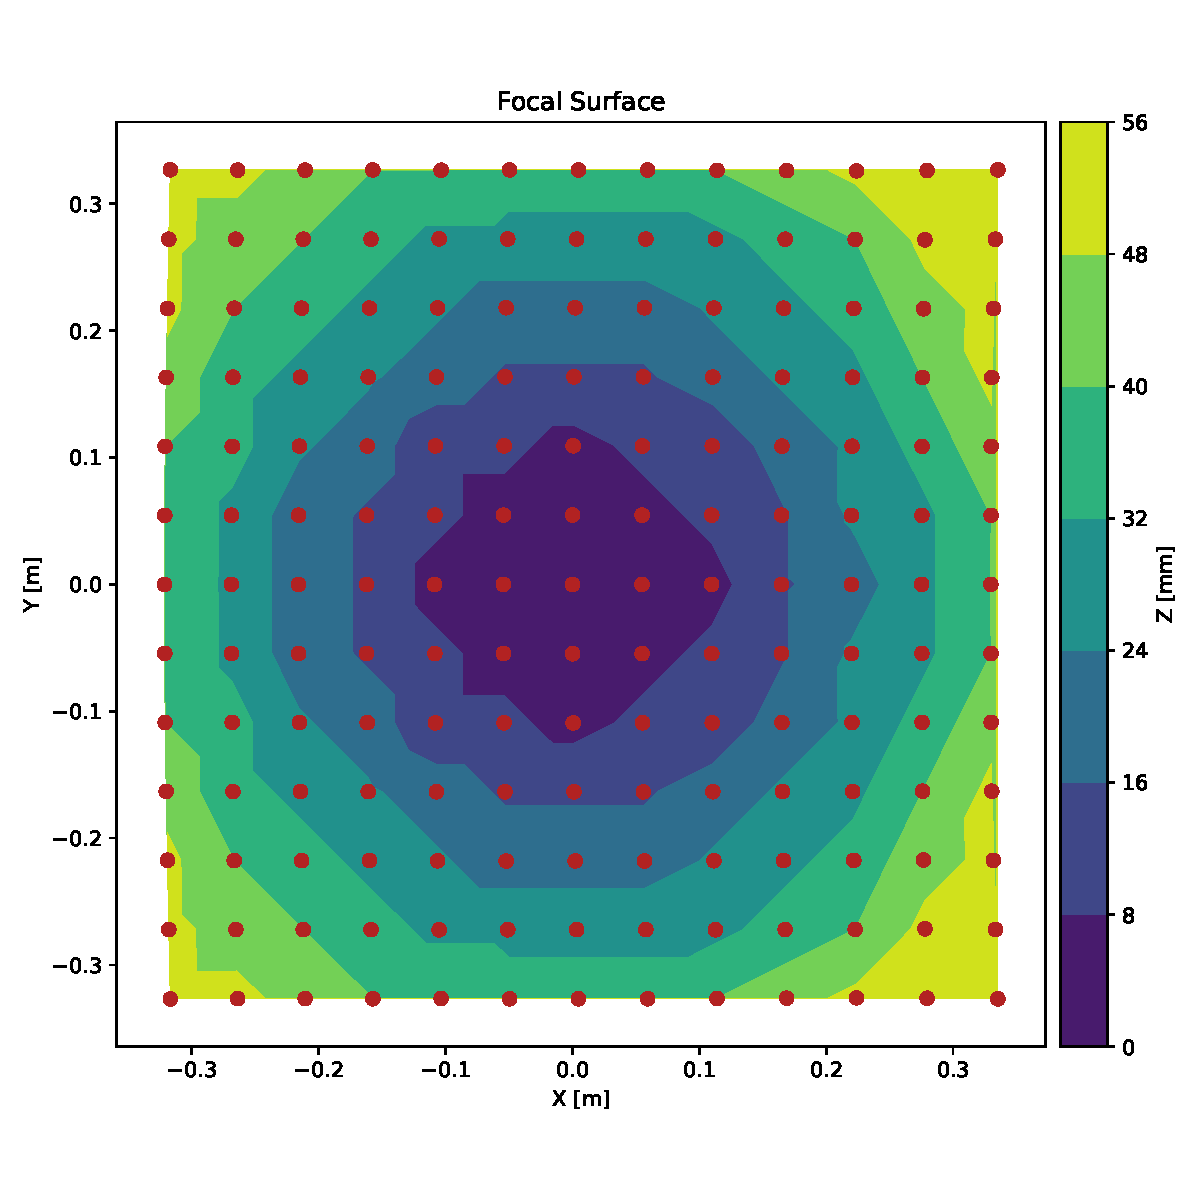
\includegraphics[scale=0.6]{../figures/ContourPlot_z.pdf}
	\caption{Contour plot dei punti sulla superficie focale in corrispondenza dei quali è stato calcolato il beam con GRASP. In rosso è evidenziata la griglia $13\text{x}13$ definita dalle componenti $x$ e $y$. Le gradazioni di colore rappresentano la coordinata spaziale $z$. Il modello di telescopio è quello mostrato in Fig.~\ref{strip}.}
	\label{cplot_fs}
\end{figure}

Per stimare il valore dei parametri ho simulato la risposta di un beam collocato su vari punti del piano focale. Questi sono espressi come coordinate $(x,y,z)$ in uno spazio cartesiano e sono rappresentati nel grafico~\ref{cplot_fs}.
I punti sono distributi su una griglia $13\text{x}13$ lungo le componenti $x$ e $y$. La griglia ha una dimensione di $\sim 70 \unit{cm}\text{x}70 \unit{cm}$, mentre la coordinata $z$ varia tra $0$ e $50 \unit{mm}$.


Nonostante abbia eseguito la medesima analisi su ciascuno dei parametri descritti nel capitolo precedente (ellitticità, FWHM rispetto a x, FWHM rispetto a y, componente copolare massima, componente cross-polare massima), riporto in questo capitolo solo i risultati relativi all'ellitticità, in quanto gli altri risultati sono molto simili.

\begin{figure}[!ht]
	\centering
	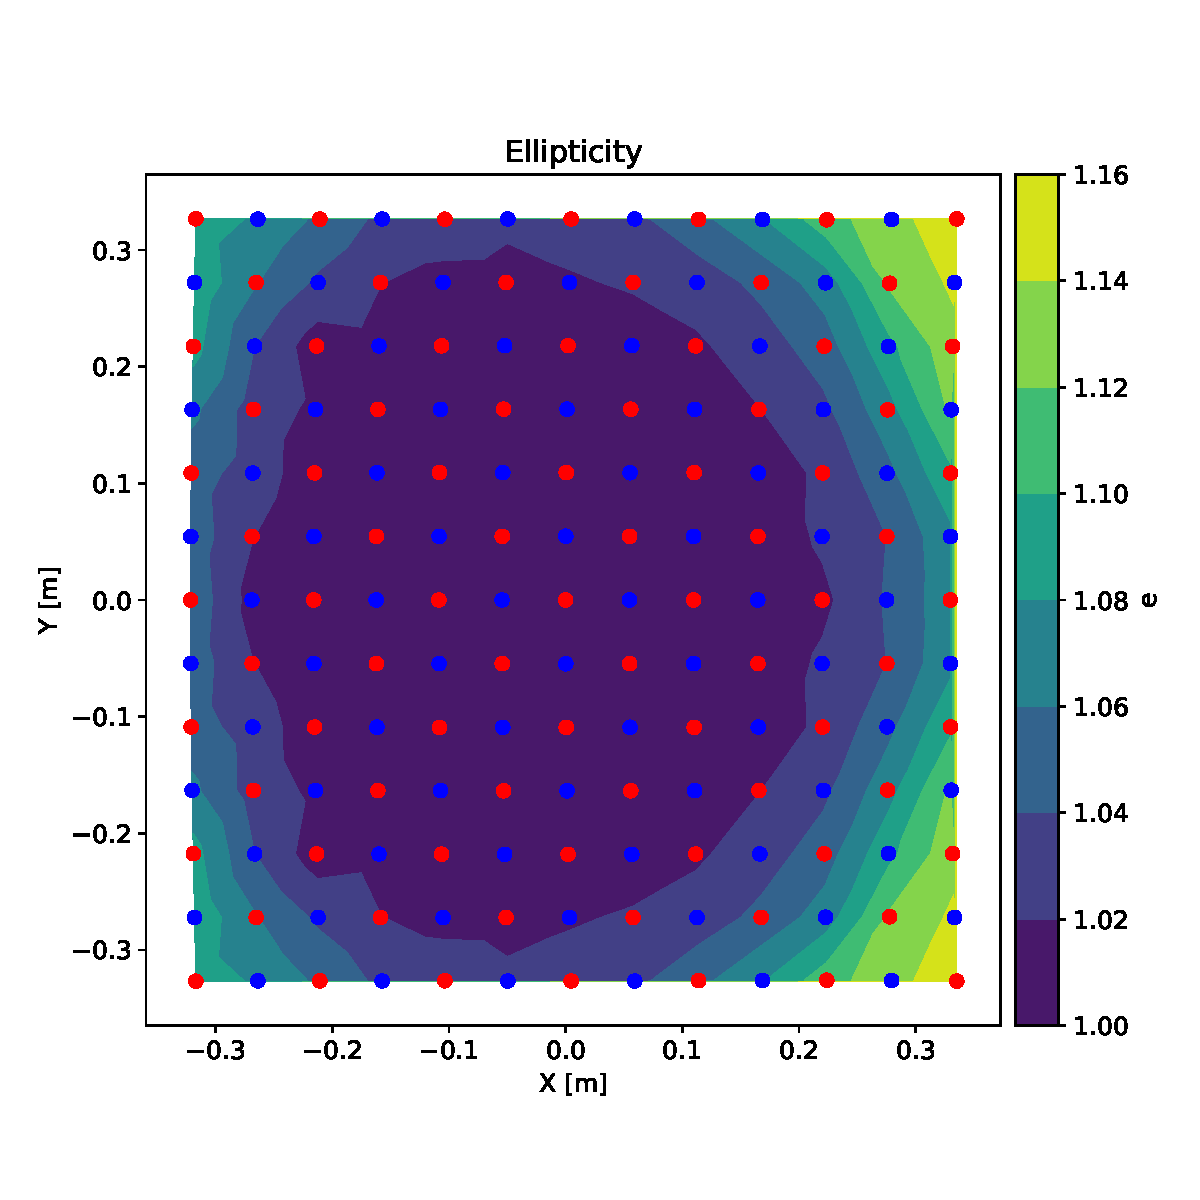
\includegraphics[scale=0.6]{../figures/ContourPlot_e.pdf}
	\caption{Contour plot dell'ellitticità. Il suo valore nei vari punti è dato dalla tabella~\ref{dataset}. In rosso sono evidenziati i punti attraverso i quali verrà effettuata l'interpolazione dei parametri del beam mentre in blu sono rappresentati i punti in corrispondenza dei quali ho cercato di prevedere le caratteristiche del beam tramite uno dei metodi descritti in questo lavoro.}
	\label{cplot_e}
\end{figure}

\begin{comment}
Manca qui un paragrafo che spieghi le premesse della simulazione. Sono tante le cose da dire: (1) hai simulato la risposta di un beam collocato su vari punti del piano focale, (2) i punti sono espressi come coordinate (x, y, z) in uno spazio cartesiano, (3) i punti sono distribuiti secondo una griglia lungo le componenti x e y, (3) mancano le dimensioni della griglia (per quanti cm si estende lungo i due assi?, qual è la variabilità dell'asse z?).
\end{comment}

    %%%%%%%%%%%%%%%%%%%  CAPITOLO 3.1  %%%%%%%%%%%%%%%%%%%

\section{Interpolazione}\label{interpolazione}
Per stimare le proprietà di un diagramma di radiazione attraverso strumenti classici di interpolazione ho utilizzato due metodi: \texttt{interp2d} del modulo \texttt{scipy.interpolate}, basato su un'interpolazione lineare tra punti adiacenti, e \texttt{curve\_fit} del modulo \texttt{scipy.optimize}, con cui ho interpolato i dati tramite un paraboloide; il diagramma in Fig.~\ref{es_interp} chiarisce la differenza tra i due approcci.
Per poter effettuare l'interpolazione dei parametri e in seguito verificare la sua bontà, ho suddivido il dataset in Fig.~\ref{dataset} in due subsets, considerando righe alterne, che ho chiamato \texttt{data\_int} e \texttt{data\_check}\footnote{I punti appartenenti a \texttt{data\_int} sono quelli indicati in rosso nel grafico~\ref{cplot_e}, mentre i punti appartenenti a \texttt{data\_int} sono quelli indicati in blu.}. Così facendo è stato possibile utilizzare metà dei dati per l'interpolazione e l'altra metà per la valutazione dell'errore tra il parametro stimato e quello esatto.

\begin{figure}[!ht]
	\centering
	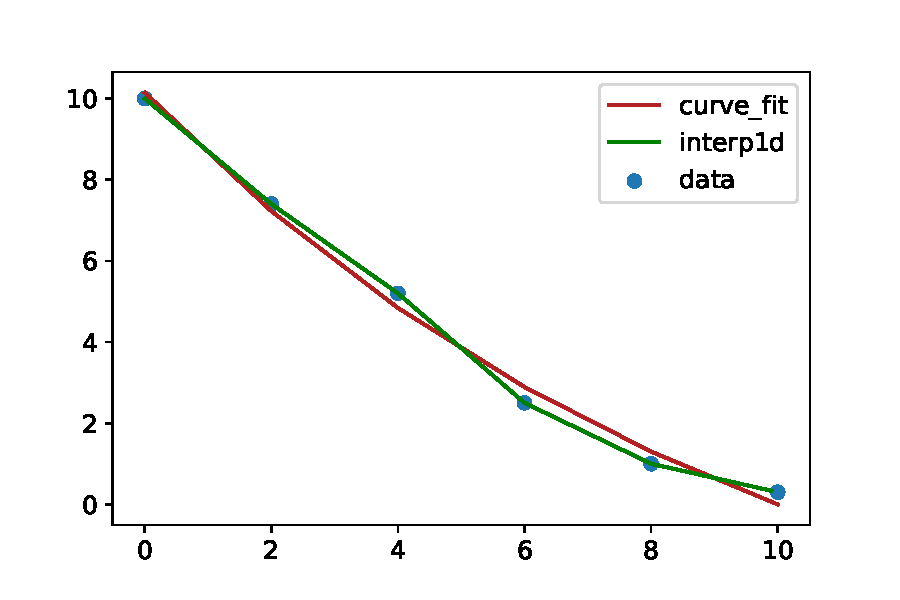
\includegraphics[scale=0.8]{../figures/EsempioInterpolazione.pdf}
	\caption{Grafico che mostra la differenza tra \texttt{interp1d} e \texttt{curve\_fit}. Il fit è stato fatto su una funzione della forma $f=a^{((b\cdot x)+c)}+d$, dove \textit{a, b, c, d} sono i parametri stimati da \texttt{curve\_fit} mentre il metodo \texttt{interp1d} stima il valore della funzione in un determinanto punto effettuando l'interpolazione tra i due punti noti ad esso adiacenti.}
	\label{es_interp}
\end{figure}

         %%%%%%%%%%%%%%%%%%%  CAPITOLO 3.1.1  %%%%%%%%%%%%%%%%%%%

\subsection{Interp2d}\label{interp2d}
Il metodo \texttt{interp2d}\footnote{\texttt{interp2d} è il corrispettivo di \texttt{interp1d} ma in due dimensioni.} effettua l'interpolazione a partire da una griglia bidimensionale\footnote{La griglia non deve essere necessariamente regolare.}, nel mio caso questa è rappresentata dalle coppie $(x,y)$ appartenti al subset \texttt{data\_int}. Una volta specificato il parametro di interesse, l'algoritmo effettua un'interpolazione lineare e ritorna una funzione in grado di prevedere il valore del parametro in nuovi punti.
La successiva analisi ha riguardato la valutazione dell'errore tra il parametro stimato nei punti $(x,y)$ appartenenti a \texttt{data\_check} e il suo valore vero. In Fig.~\ref{err_interp2d} è mostrato l'errore assoluto relativo all'ellitticità.
Si nota che i punti della prima riga a partire dall'alto sono quelli affetti da errore massimo e, come verrà specificato nella Sez.~\ref{risultati_interpolazione}, tali anomalie di bordo hanno determinato la scelta del metodo \texttt{curve\_fit} come termine di paragone con le reti neurali.
\begin{figure}[!ht]
	\centering
	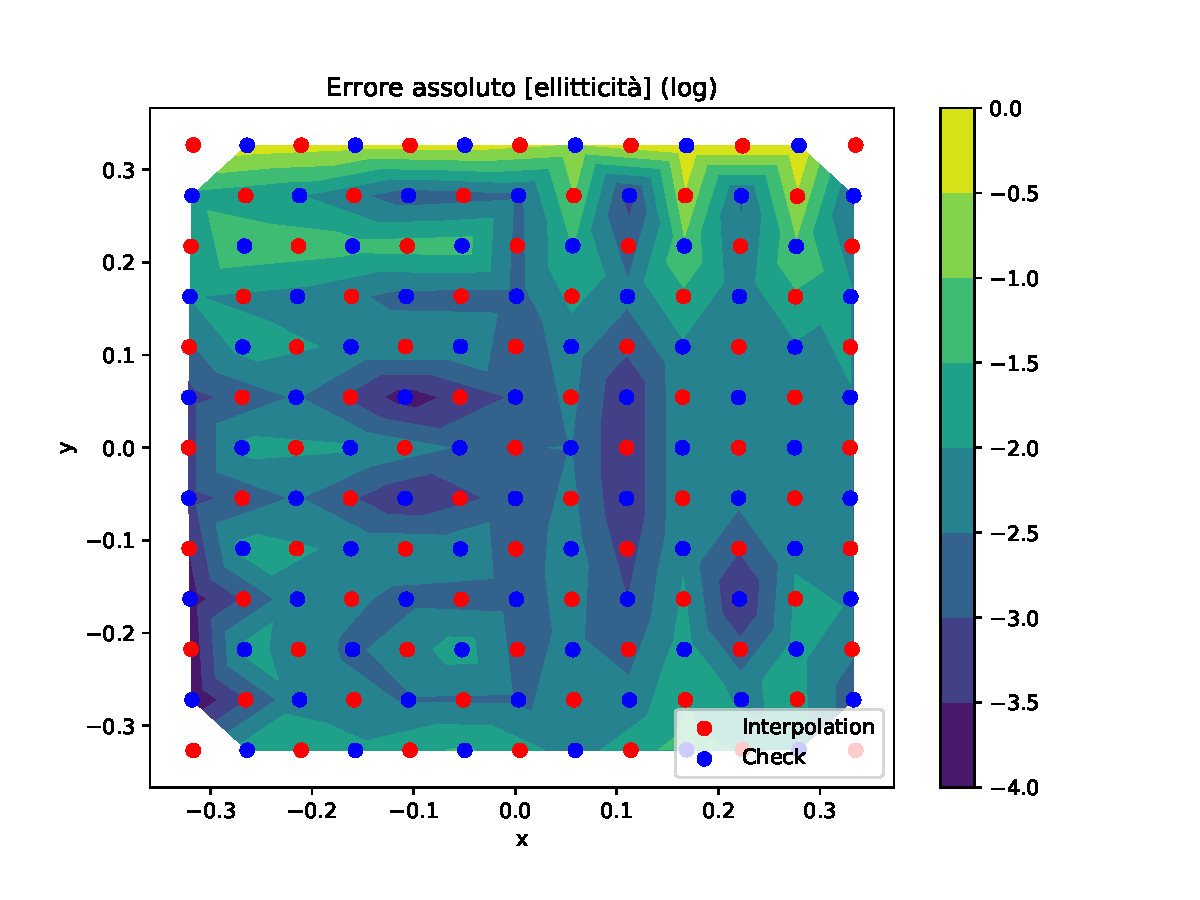
\includegraphics[scale=0.6]{../figures/errore_assoluto_ell.pdf}
	\caption{Contour plot in scala logaritmica dell'errore assoluto tra ellitticità interpolata tramite il metodo \texttt{interp2d} e ellitticità corretta. In rosso sono evidenziati i punti attraverso i quali è stata effettuata l'interpolazione mentre in blu sono rappresentati i punti nei quali è stato valutato l'errore.}
	\label{err_interp2d}
\end{figure}


A causa del funzionamento di \texttt{interp2d} non è possibile ottenere stime affidabili se il punto $(x, y)$ cade al di fuori del poligono convesso che racchiude i punti usati per l'interpolazione. Nel grafico~\ref{es_interp} non è infatti possibile stimare il valore di $y$ per $x>10$ o $x<0$.
\`E quindi conveniente effettuare un campionamento, tramite i metodi di simulazione (vedi Sez.~\ref{simulazioni}), soprattutto al bordo della regione di spazio di interesse. In tal modo si è certi che i punti sui quali vado a stimare i parametri appartengono al dominio dei punti simulati.

         %%%%%%%%%%%%%%%%%%%  CAPITOLO 3.1.2  %%%%%%%%%%%%%%%%%%%

\subsection{Curve Fit}\label{curve_fit}
\begin{figure}[!ht]
	\centering
	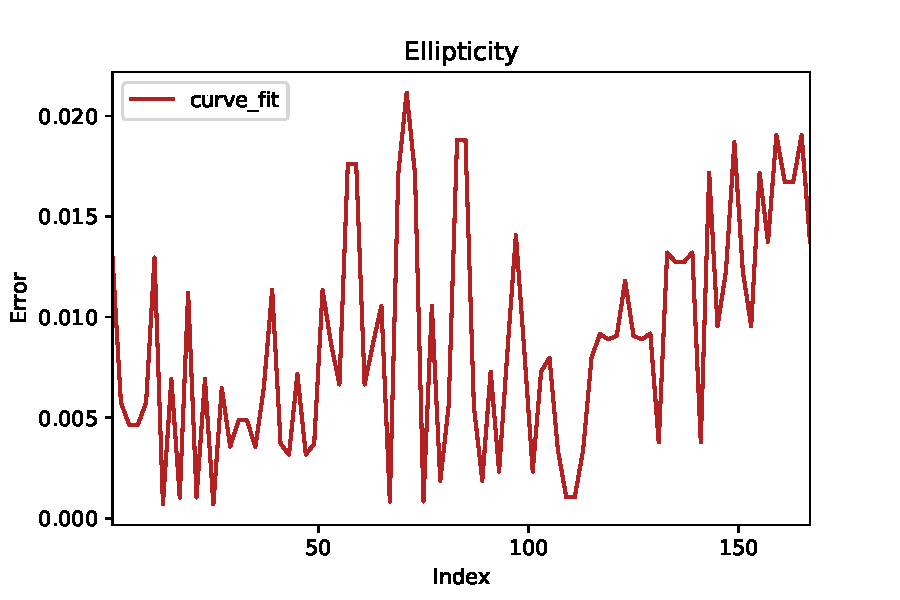
\includegraphics[scale=0.7]{../figures/error_curve_fit.pdf}
	\caption{Plot che mostra l'errore assoluto tra ellitticità interpolata tramite il metodo \texttt{curve\_fit} e ellitticità corretta.}
	\label{err_curve_fit}
\end{figure}
Il metodo \texttt{curve\_fit} permette di fittare i dati con una funzione tramite il metodo dei minimi quadrati. Il metodo restituisce i valori ottimali dei parametri \texttt{popt} che minimizzano la discrepanza $f(xdata, *popt) - ydata$\footnote{In particolare \textit{xdata} è una coppia $(x,y)$ e \textit{ydata} è il valore del parametro di interesse.}. Anche in questo caso ho utilizzato i due subset, \texttt{data\_int} e \texttt{data\_check}, per effettuare rispettivamente il fit e la valutazione dell'errore. Nel mio caso il fit è stato eseguito su un paraboloide in quanto questo richiama l'andamento dell'ellitticità.
        %%%%%%%%%%%%%%%%%%%  CAPITOLO 3.1.3  %%%%%%%%%%%%%%%%%%%

\subsection{Risultati dell'interpolazione}\label{risultati_interpolazione}
Ho poi comparato i due metodi di interpolazione.
\begin{figure}[!ht]
	\centering
	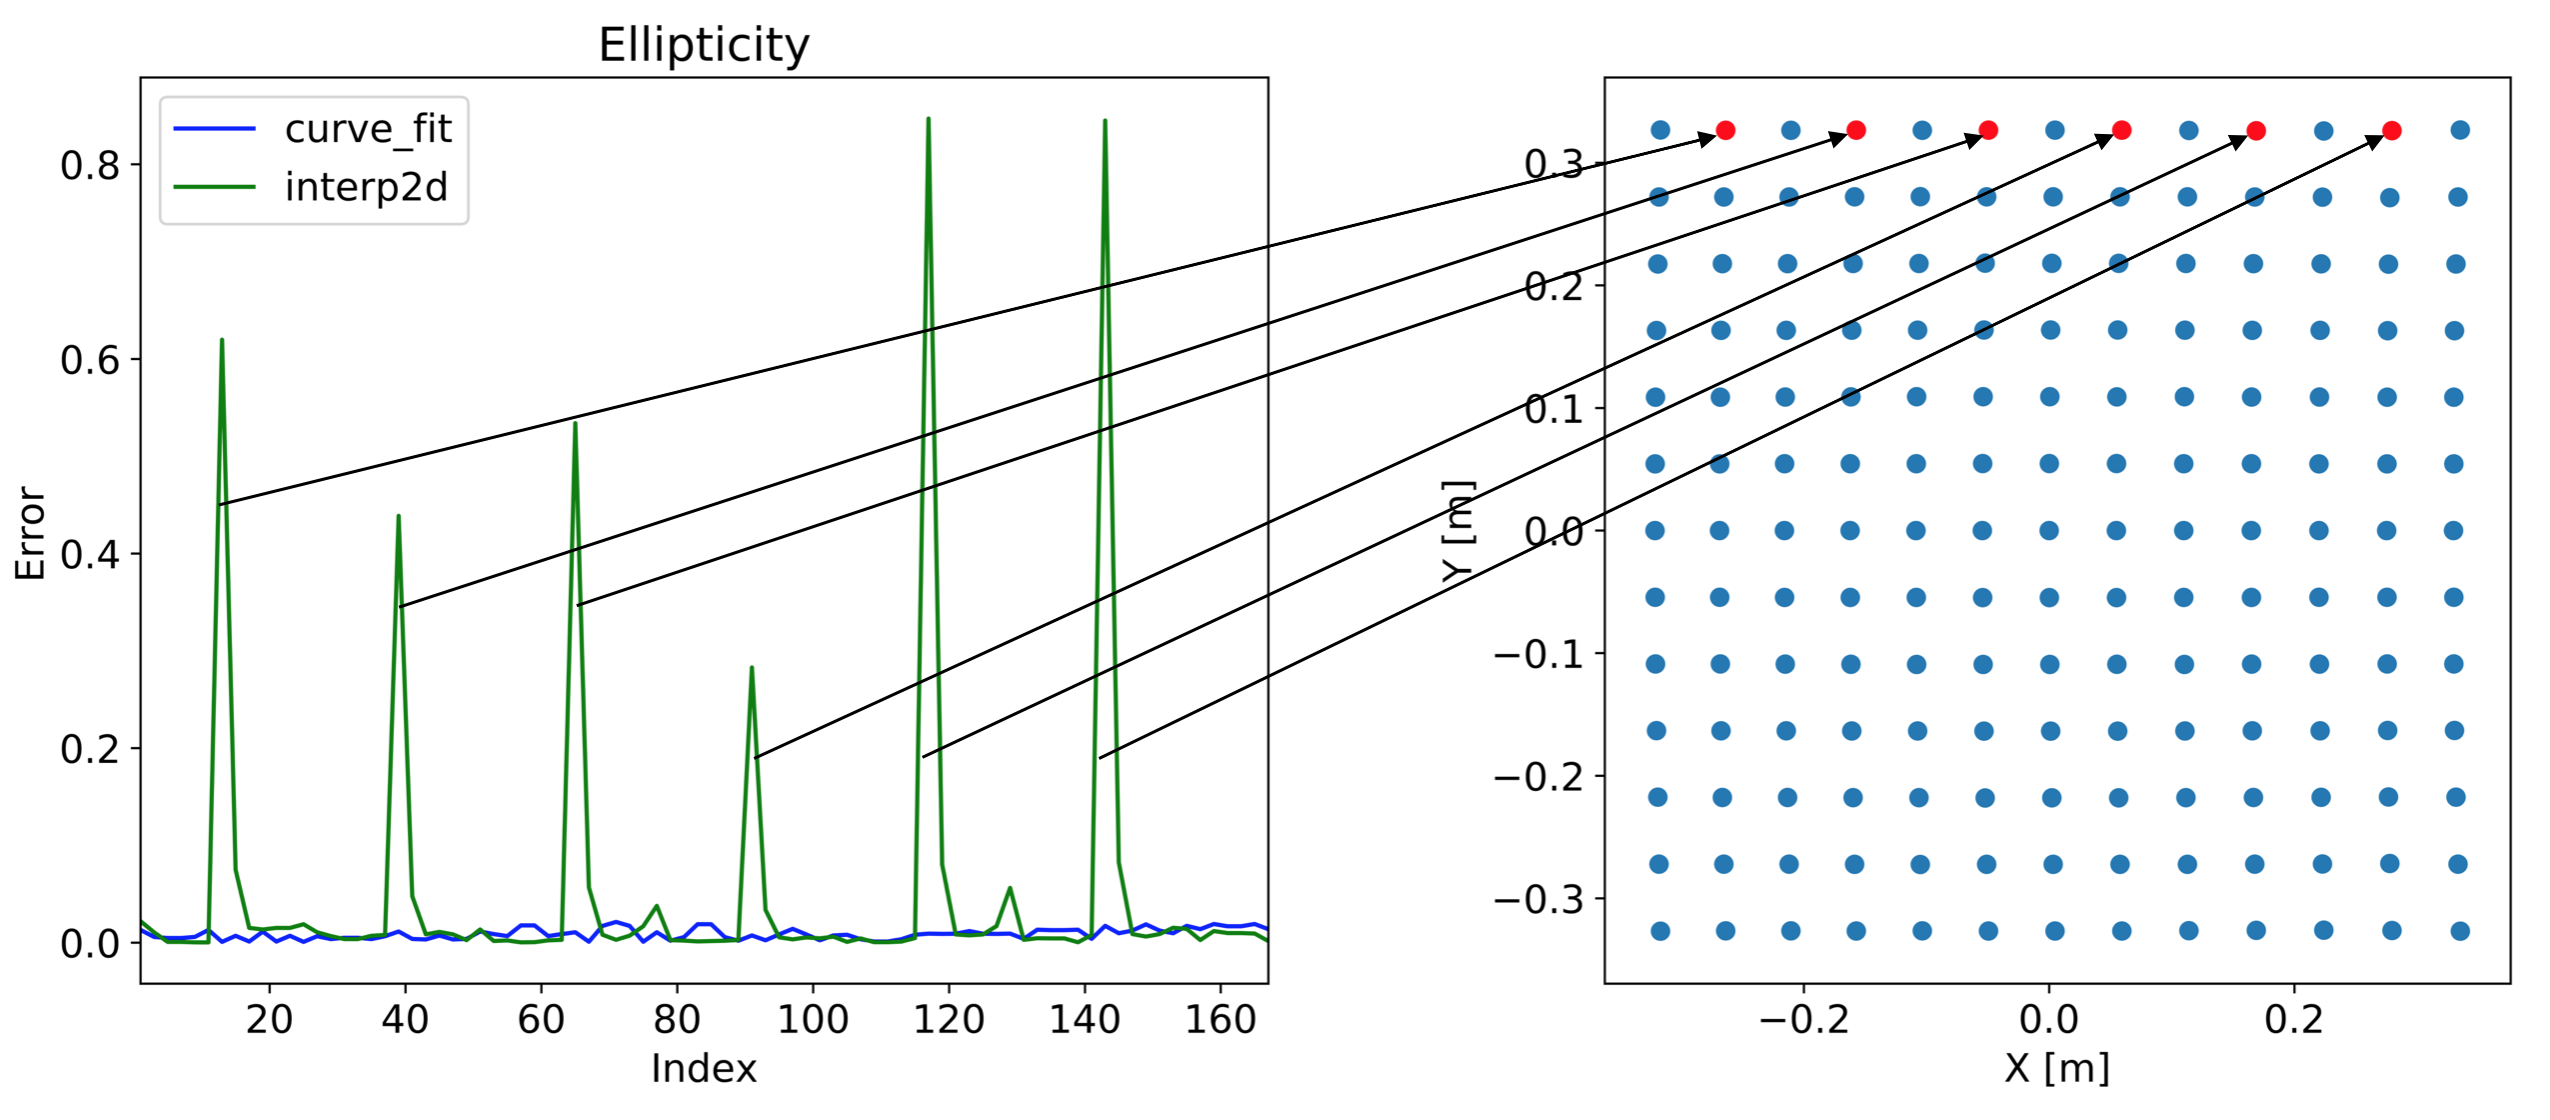
\includegraphics[width=\linewidth]{../figures/punti_prob.png}
	\caption{Confronto dell'errore prodotto dai due metodi di interpolazione relativo all'ellitticità. I punti indicati dalle frecce sono i responsabili dei picchi della curva verde.}
	\label{err_int}
\end{figure}
\newline
In Fig.~\ref{err_int} sono confrontate le curve che rappresentano l'errore tra dato interpolato e dato corretto per i due metodi utilizzati. Si nota immediatamente che la curva relativa a \texttt{interp2d} è sensibilmente peggiore di quella relativa \texttt{curve\_fit}. Questo è dovuto alla presenza di alcuni picchi problematici che risultano essere causati dai punti sul bordo.
Analizzando infatti più in dettaglio il comportamento del metodo \texttt{interp2d} è possibile mostrare che i punti affetti da errore maggiore sono punti di bordo. L'analisi è stata fatta plottando il valore interpolato e valore esatto del parametro per ogni riga di punti della griglia $13\text{x}13$.
In Fig.~\ref{plot_row} è mostrato il diverso comportamento di \texttt{interp2d} per una riga di punti di bordo e una riga di punti interni alla griglia.

\begin{figure}[!ht]
\centering
	\begin{subfigure}{\textwidth}
	    \centering
	    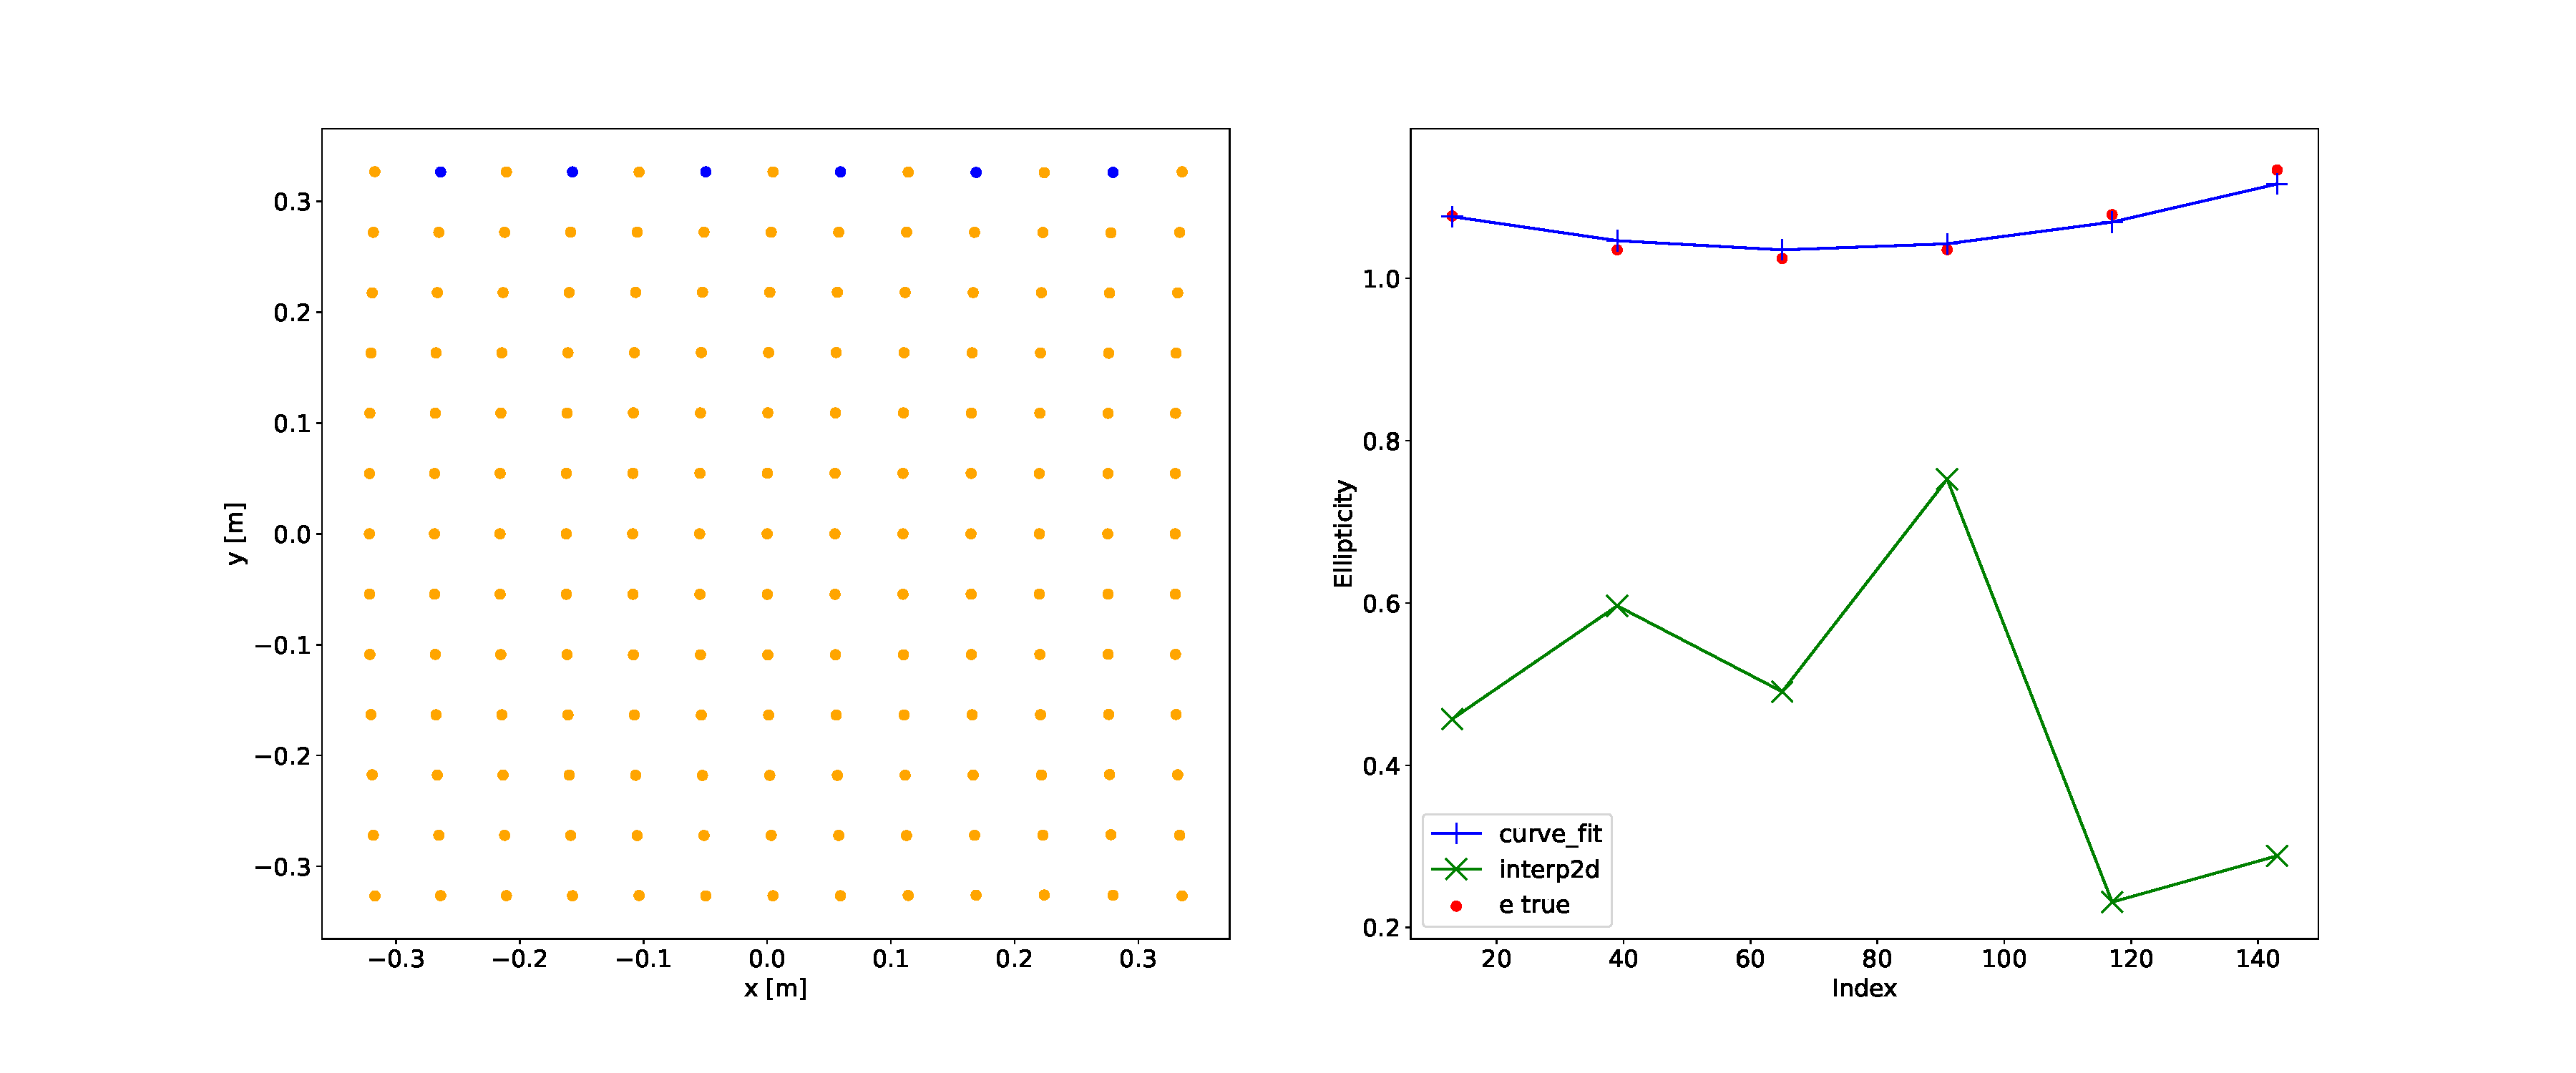
\includegraphics[width=\linewidth]{../figures/row_bordo.pdf}
	    \caption{Punti di bordo}
	    \label{plot_row_bordo}
	\end{subfigure}
\newline
	\begin{subfigure}{\textwidth}
		\centering
	    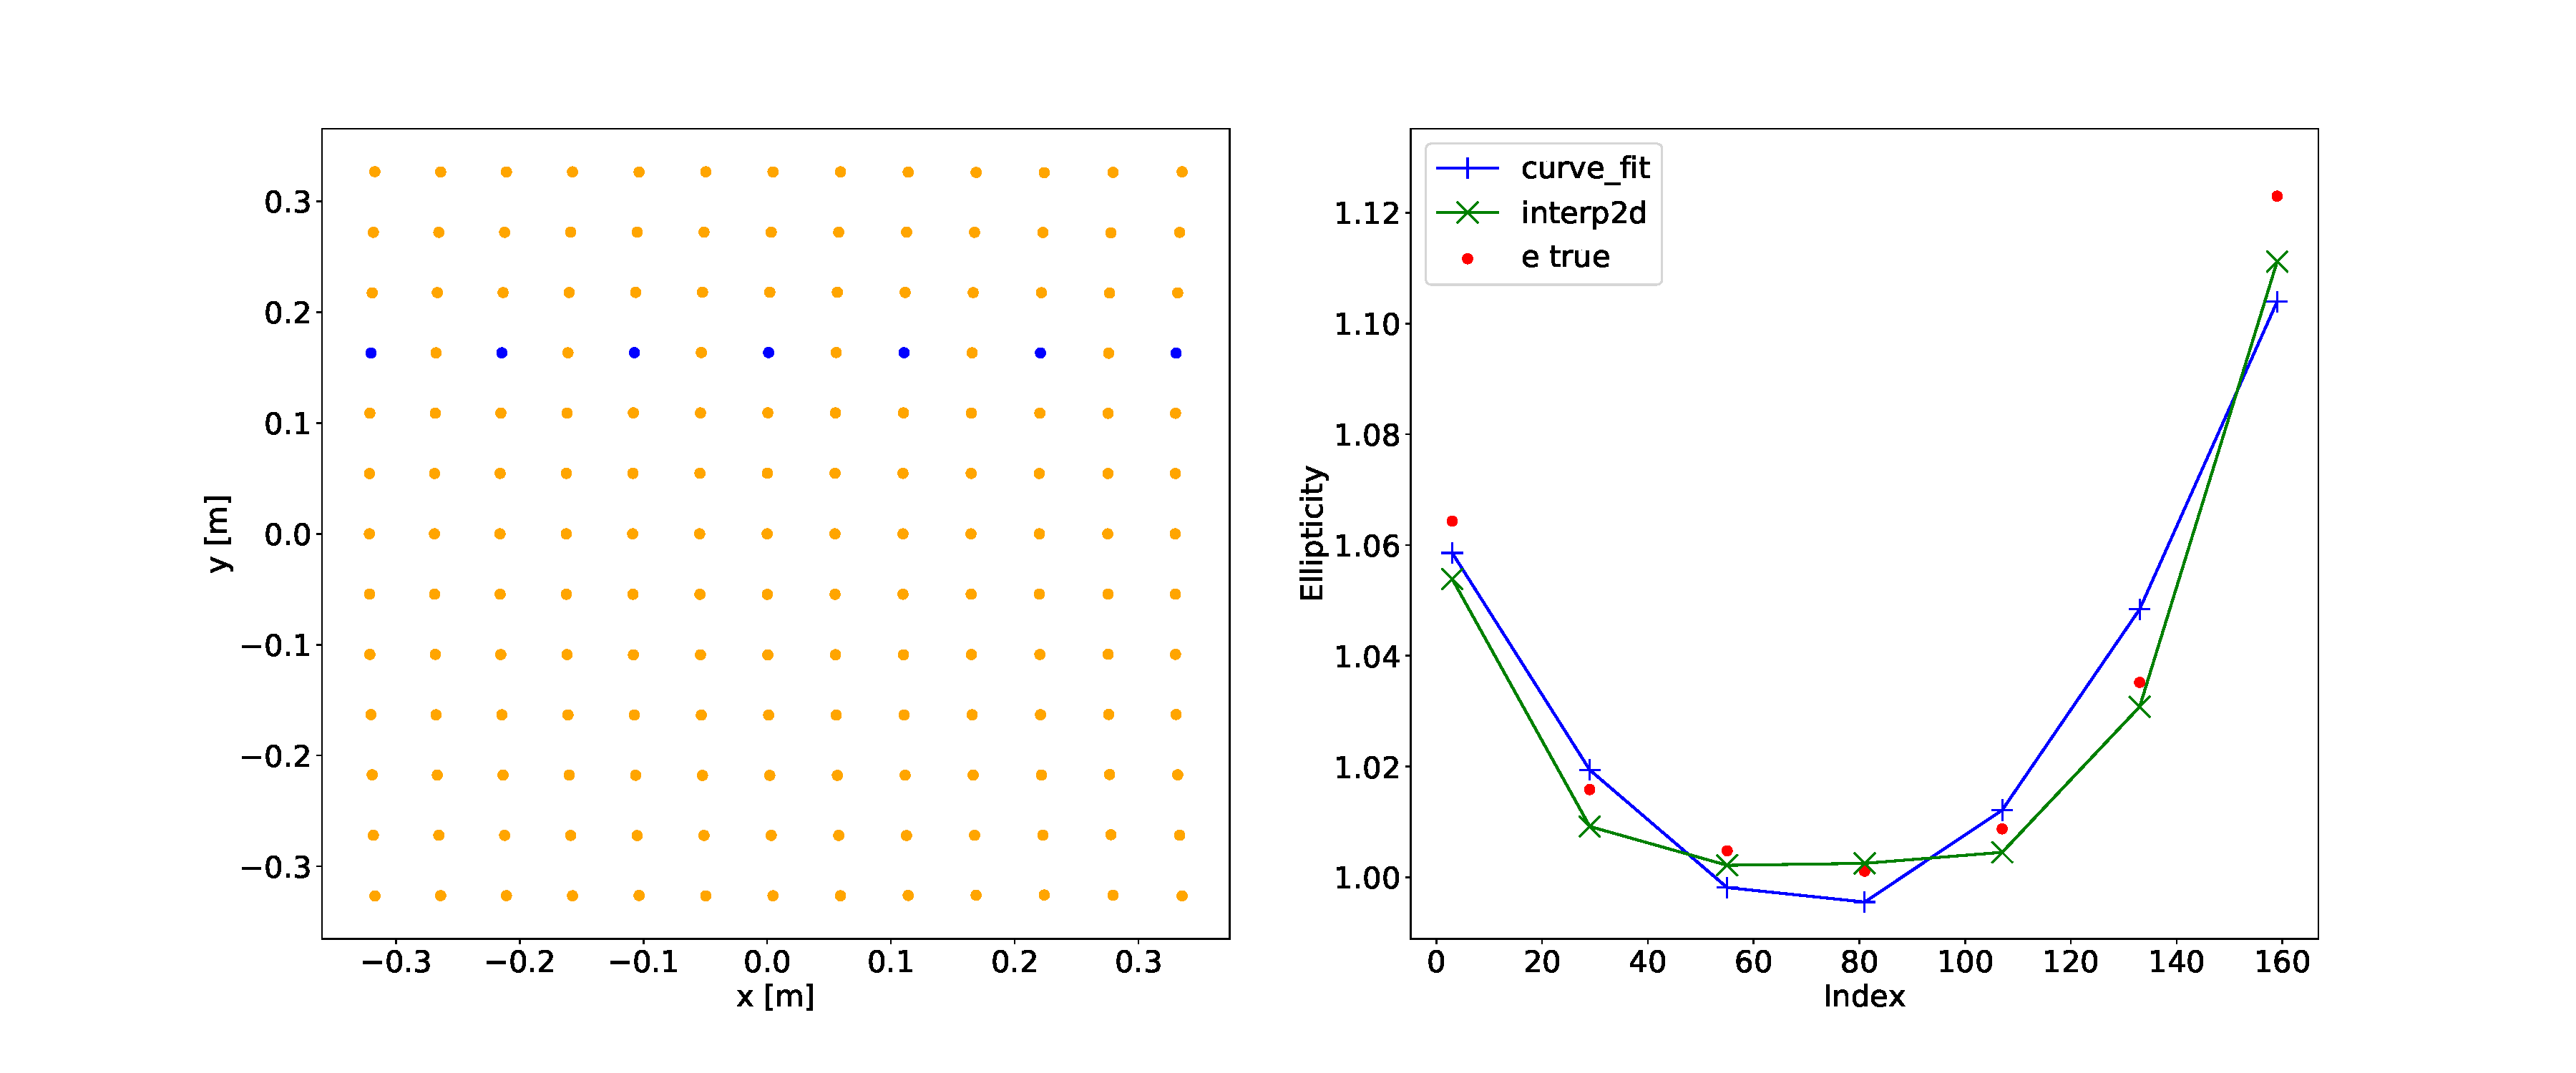
\includegraphics[width=\linewidth]{../figures/row_interno.pdf}
		\caption{Punti interni}
		\label{plot_row_interno}
	\end{subfigure}
	\caption{Plot del valore dell'ellitticità per due diverse righe di punti. Sono indicati il valore vero, in rosso, il dato previsto con \texttt{interp2d}, in verde e con \texttt{curve\_fit}, in blu. Nel grafico~\ref{plot_row_bordo} è mostrato l'andamento dell'ellitticità per una riga di punti di bordo mentre nel grafico~\ref{plot_row_interno} viene analizzata l'ellitticità di una riga interna della griglia di punti. Nel grafico sulla sinistra sono evidenziati in blu i punti, sulla riga analizzata, su cui è effettuata la verifica dell'interpolazione. Al variare del parametro variano i punti problematici per \texttt{interp2d} ma l'andamento generale rimane lo stesso, il presente plot è dunque da considerarsi rappresentativo di tutti i casi analizzati.}
	\label{plot_row}
\end{figure}

Per poter confrontare nuovamente gli errori dei due metodi di interpolazione ho creato un subset del dataset iniziale rimuovendo i punti più esterni: \texttt{data\_mask}. Il nuovo dataset è costituito dai punti blu raffigurati in Fig.~\ref{data_mask}.

\begin{figure}[!ht]
	\centering
	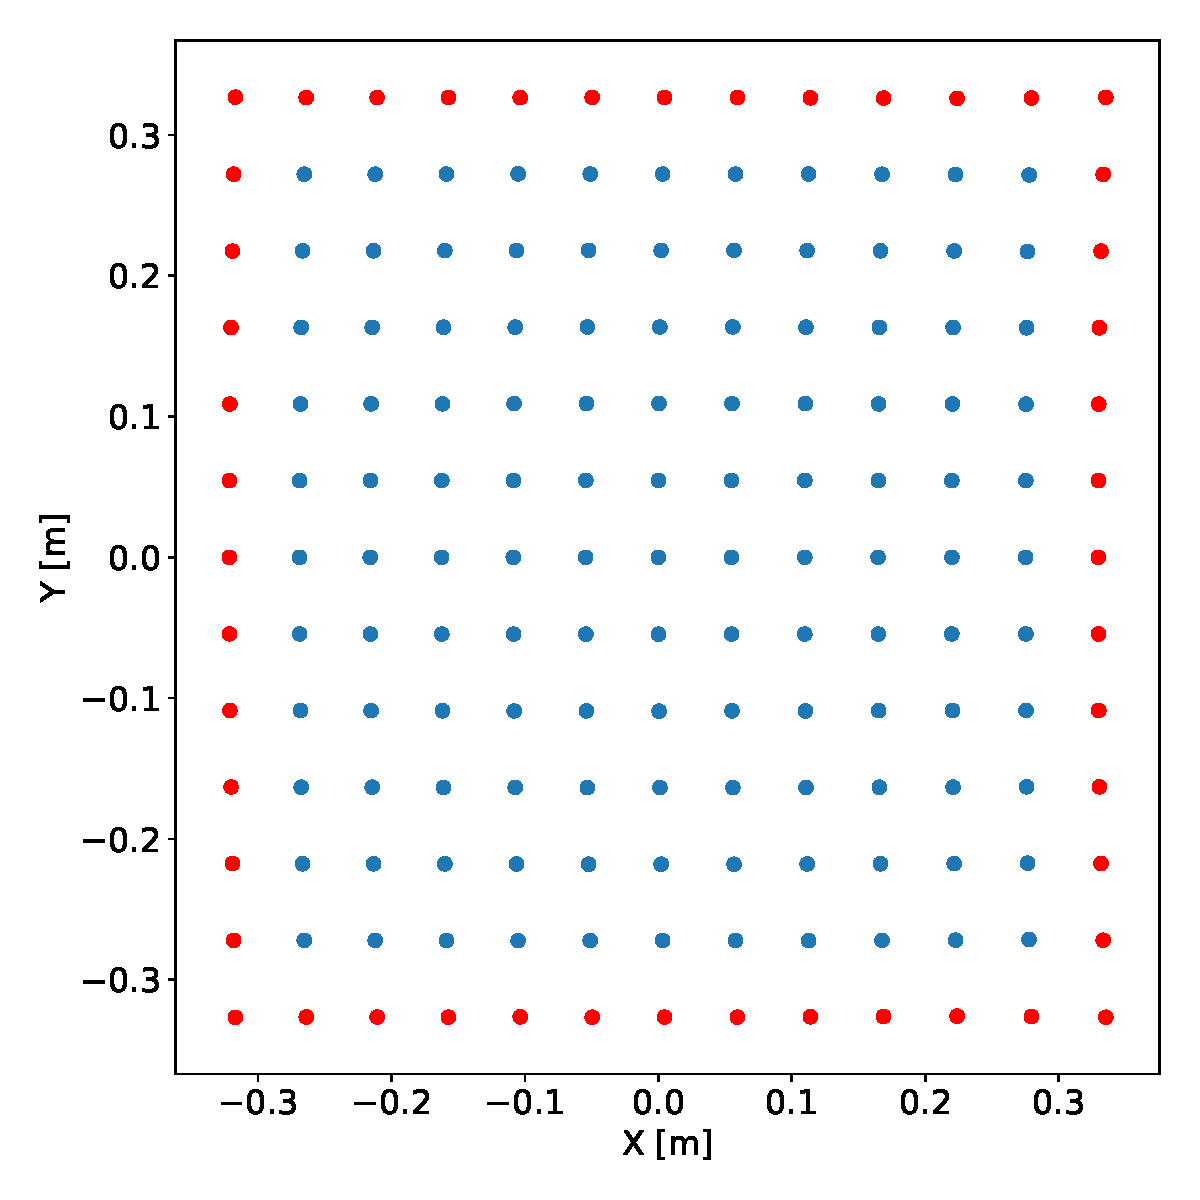
\includegraphics[width=0.6\linewidth]{../figures/PuntiMask.pdf}
	\caption{Rappresentazione dei punti appartenenti al subset \texttt{data\_mask}, in blu. In rosso sono rappresentati i punti di bordo che ho rimosso.}
	\label{data_mask}
\end{figure}

Il passaggio successivo è stato plottare nuovamente l'errore come in Fig.~\ref{err_int} e il risultato ottenuto è mostrato in Fig.~\ref{err_int_mask}.

\begin{figure}[!ht]
	\centering
	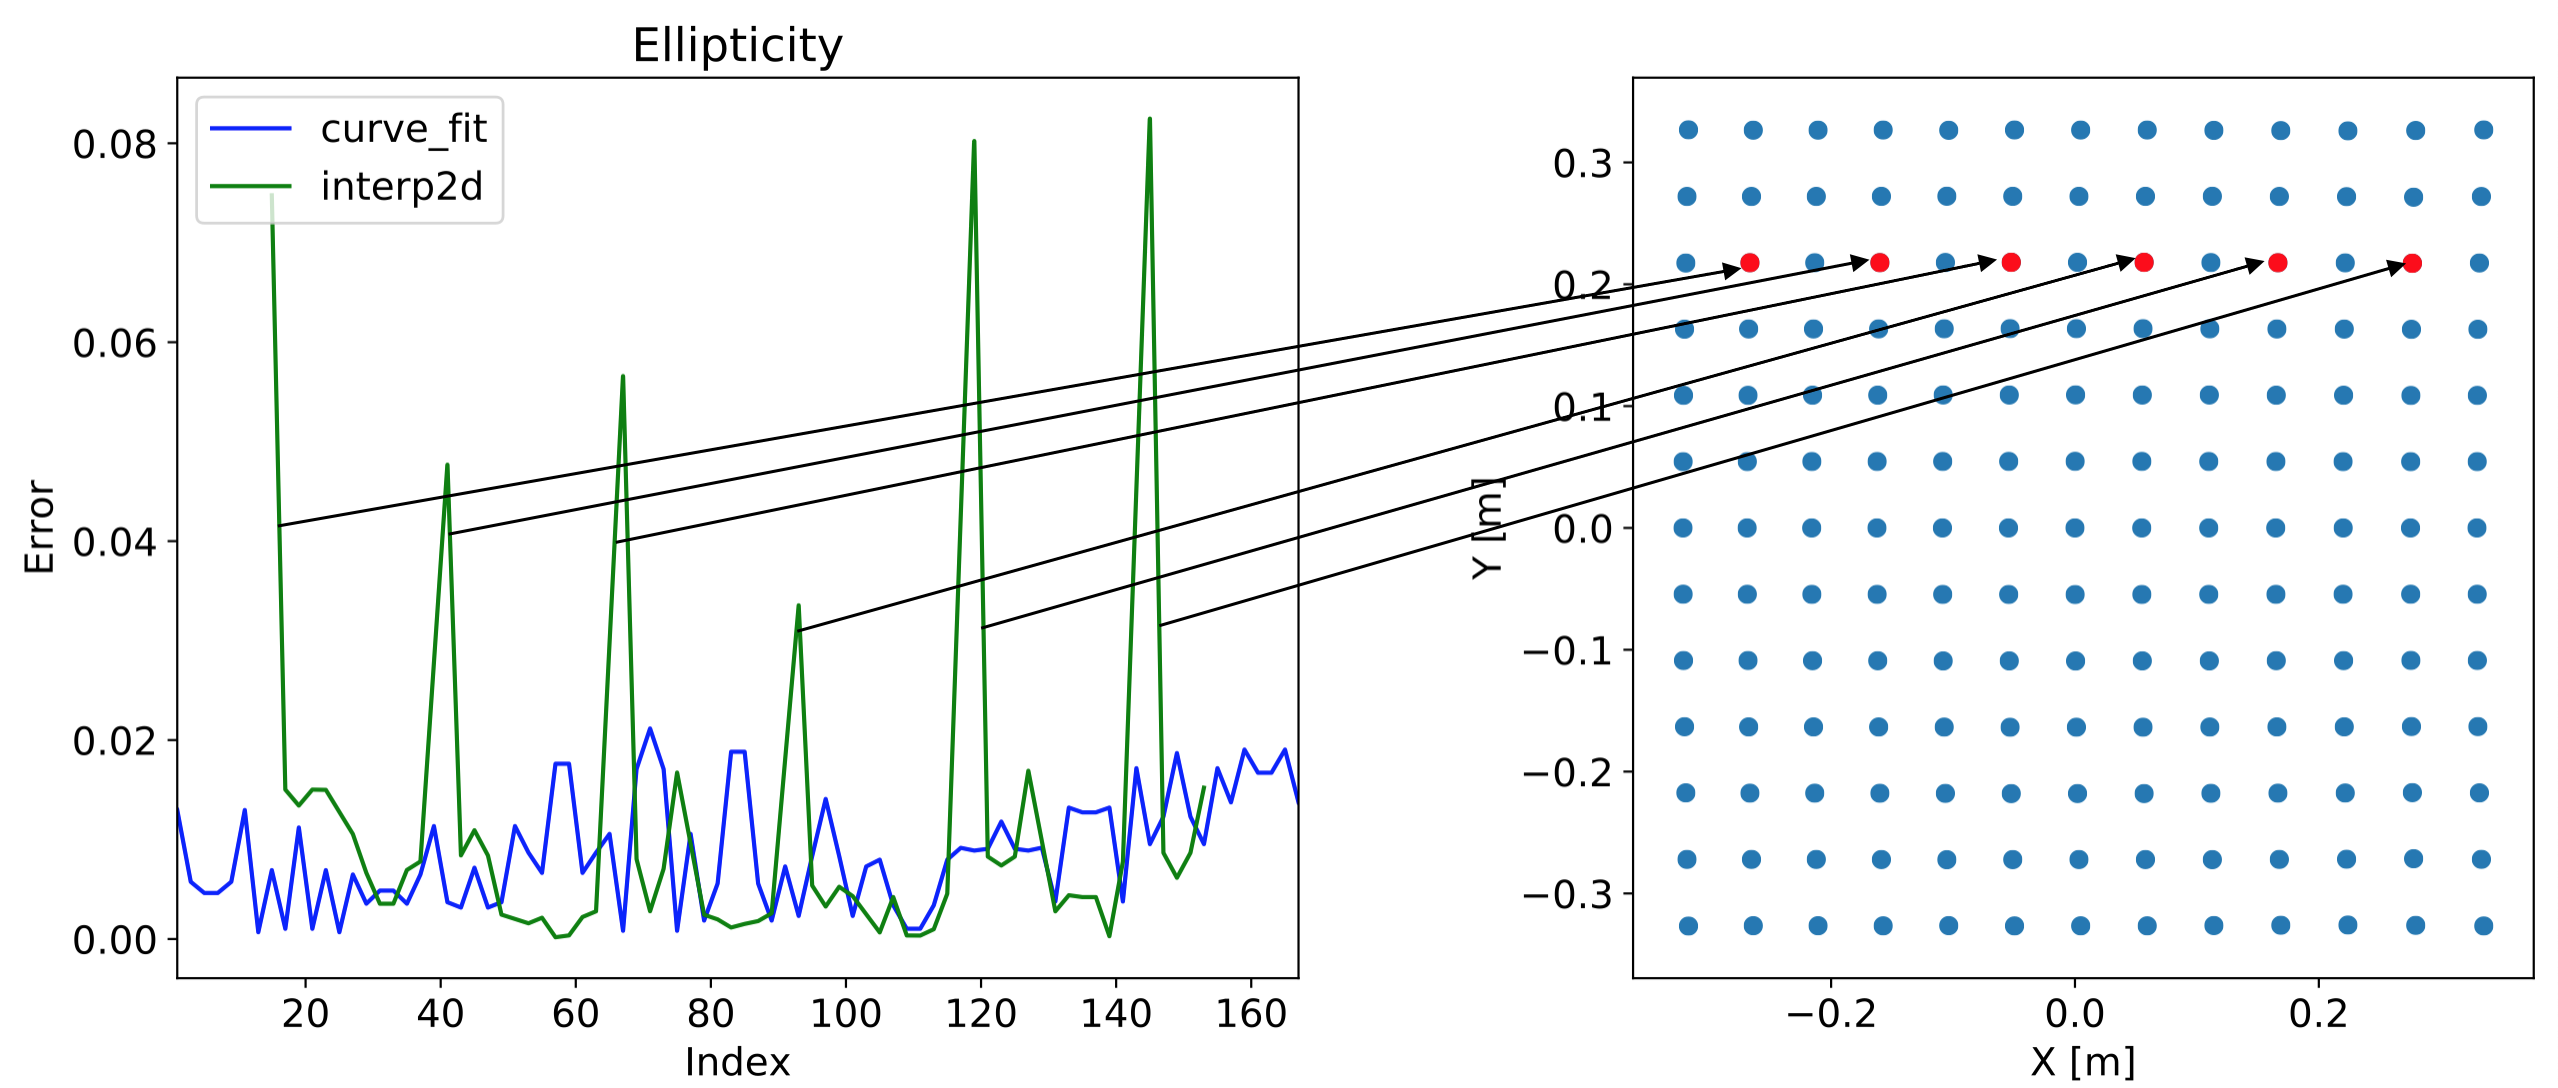
\includegraphics[width=\linewidth]{../figures/PuntiProblematiciMask.png}
	\caption{Confronto dell'errore relativo ai due metodi di interpolazione dopo aver rimosso i punti di bordo. I punti indicati dalle frecce sono i responsabili dei picchi della curva verde.}
	\label{err_int_mask}
\end{figure}

Il plot in Fig.~\ref{err_int_mask} mostra ancora dei punti nei quali l'errore di \texttt{interp2d} è molto maggiore rispetto a quello di \texttt{curve\_fit}, per tale motivo ho deciso di considerare esclusivamente il metodo \texttt{curve\_fit} come termine di paragone tra i risultati relativi all'interpolazione e quelli relativi alle reti neurali, come verrà mostrato nella sezione~\ref{risultati}.

\newpage
     %%%%%%%%%%%%%%%%%%%  CAPITOLO 3.2  %%%%%%%%%%%%%%%%%%%
\section{Reti neurali}\label{reti_neurali}
In questa sezione mostro come ho creato le architetture delle reti neurali utilizzate per effettuare la regressione, come ho verificato la loro validità, come ho gestito i dati a disposizione per definire \texttt{training set} e \texttt{validazion set} e come ho implementato il processo di training. Infine presenterò il confronto dei risultati ottenuti tramite l'utilizzo dell'interpolazione e delle reti (~\ref{risultati}).

        %%%%%%%%%%%%%%%%%%%  CAPITOLO 3.2.1  %%%%%%%%%%%%%%%%%%%

\subsection{Architettura della rete}\label{architettura}
Quando si costruisce una rete neurale di tipo feed-forward (il tipo usato in questo lavoro) è necessario definire alcuni elementi che andranno a caratterizzare una particolare architettura di rete.
Tali elementi sono:
\begin{itemize}
	\item La dimensione dell'\textit{input layer}.
	\item La dimensione dell'\textit{output layer}.
	\item Il numero di \textit{hidden layers}.
	\item Il numero di \textit{neuroni} per ogni hidden layer.
	\item La \textit{funzione di attivazione}.
	\item L'\textit{optimizer}.
	\item La \textit{loss function}.
\end{itemize}
La scelta dei loro valori non è mai univoca, non esiste una regola fissa per avere la ricetta perfetta che porta ai risultati migliori.
Nel mio lavoro di tesi ho utilizzato 6 diverse architetture; alcuni degli elementi appena citati sono stati mantenuti invariati per ogni architettura\footnote{L'input, per esempio, è sempre una coppia (x, y) che definisce la posizione del beam sul piano focale, mentre l'output è un singolo valore di un particolare parametro in quel punto.}, mentre altri sono stati modificati.


Per poter decrivere al meglio la scelta delle architetture è necessario fare alcune osservazioni.
Uno dei problemi più diffusi nell'ambito delle reti neurali è quello dell'\textbf{overfitting}. Si va incontro ad overfitting quando, per esempio, si utilizza un numero estremamente elevato di neuroni se confrontato con gli elementi che si hanno a disposizione per il training.
Ogni neurone è infatti caratterizzato da due parametri liberi (\textit{weight} e \textit{bias}), la presenza di un elevato numero di parametri liberi fa si che la rete impari perfettamente la corrispondenza tra input e output degli elementi nel training set, ma in tal modo si perde il carattere predittivo necessario per ottenere risultati validi. La dimensione del \textit{trainig set} andrà dunque a fissare un limite superiore del numero di neuroni totali della rete.
Per migliorare la convergenza della rete ho normalizzato i valori di output come spiegato nella sezione~\ref{pre_training}.
Non è stato invece necessario normalizzare l'input poiché l'intervallo di valori\footnote{Sia i valori di $x$ che di $y$ oscillano tra $-0.34$ \unit{m} e $+0.34$ \unit{m}.} non è sembrato così ristretto da richiedere una normalizzazione.


Con tali premesse è ora possibile giustificare le scelte fatte nella definizione dell'architettura delle reti. I parametri rimasti sempre invariati sono:
\begin{itemize}
	\item Dimensione dell'\textbf{input layer}: 2
	\item Dimensione dell'\textbf{output layer}: 1
	\item \textbf{Optimizer}: \texttt{optim.Adam}\footnote{\`E uno degli \textit{optimizer} forniti da \textit{PyTorch}.}
	\item \textbf{Loss function}: \texttt{MSELoss}\footnote{Errore quadratico medio.}
\end{itemize}
Le 6 architetture costruite sono state ottenute tramite una diversa combinazione di funzioni di attivazione e numero di hidden layers. Le funzioni di attivazione che ho utilizzato sono la \textbf{Tanh} e \textbf{Sigmoid}, rappresentate in Fig.~\ref{act_fun}. Per ogni funzione di attivazione ho considerato 3 reti con un numero crescente di hidden layers. Al variare del numero di hidden layers ho modificato il numero di neuroni relativo ad ogni layer. Le architetture finali sono riportate in tabella~\ref{architetture}.

\begin{table}[!ht]
	\centering
	\begin{tabular}{||c | c | c||}
	\hline
	Funzione d'attivazione & \# hidden layers & \# neuroni/hidden layer \\
	\hline\hline
	Tanh & 1 & 7 \\
	\hline
	Tanh & 2 & 4 \\
	\hline
	Tanh & 3 & 3 \\
	\hline
	Sigmoid & 1 & 7 \\
	\hline
	Sigmoid & 2 & 4 \\
	\hline
	Sigmoid & 3 & 3 \\
	\hline
	\end{tabular}
	\caption{Rappresentazione schematica delle architetture costruite.}
	\label{architetture}
\end{table}


\begin{figure}[!ht]
\centering
	\begin{subfigure}{0.45\textwidth}
	    \centering
	    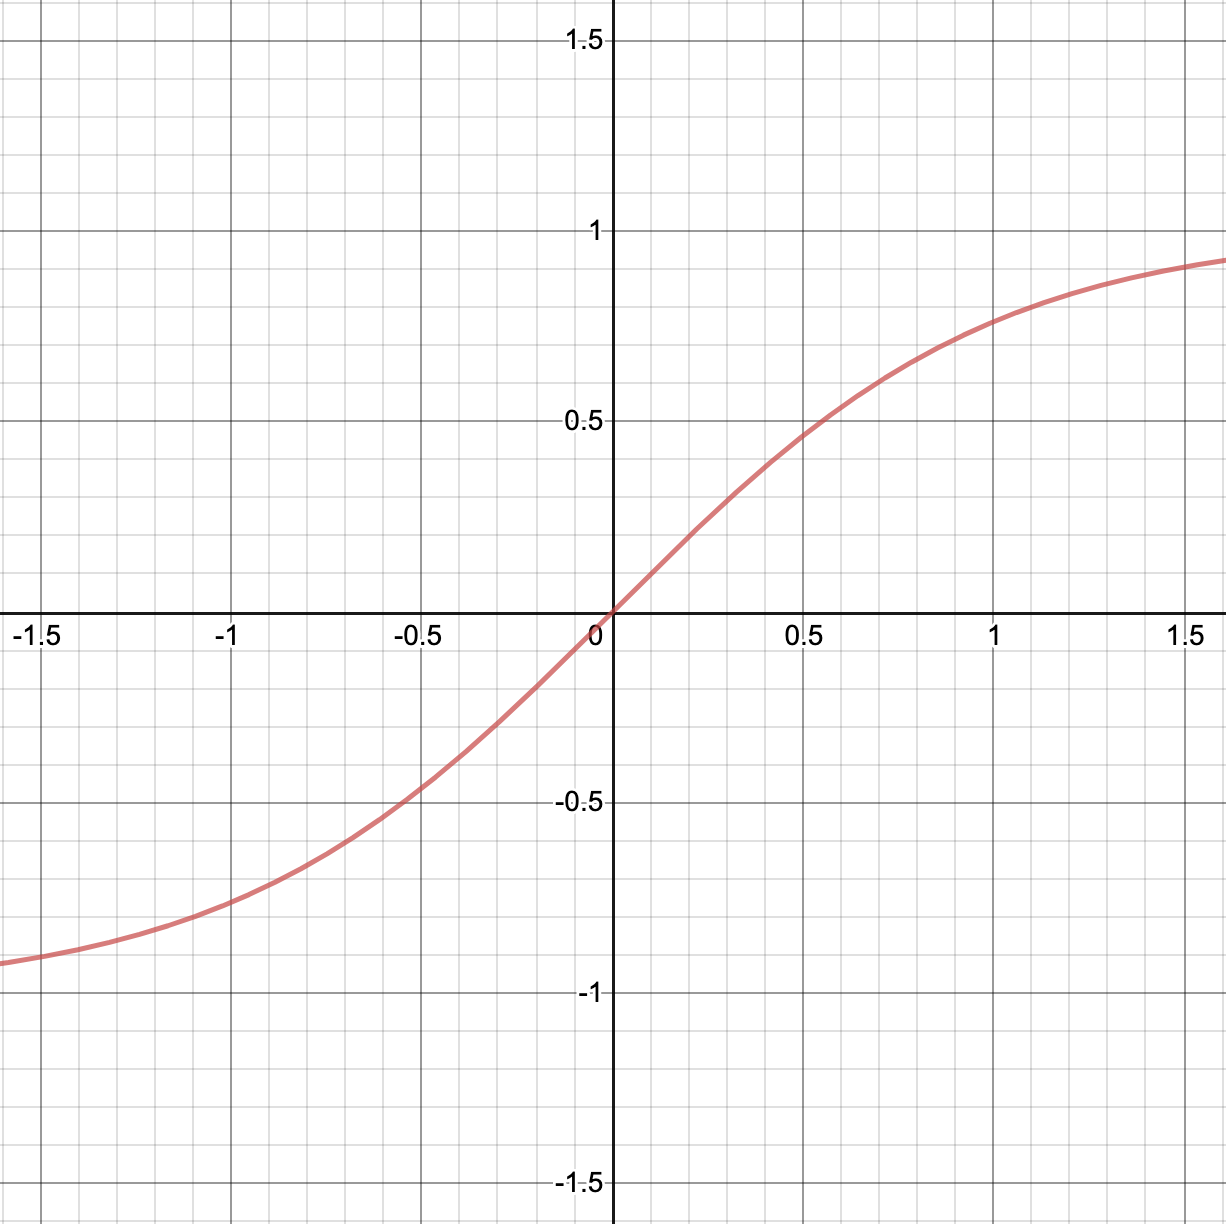
\includegraphics[width=\linewidth]{../figures/tanh.png}
	    \caption{\texttt{Tanh}}
	    \label{tanh}
	\end{subfigure}
	\begin{subfigure}{0.45\textwidth}
		\centering
	    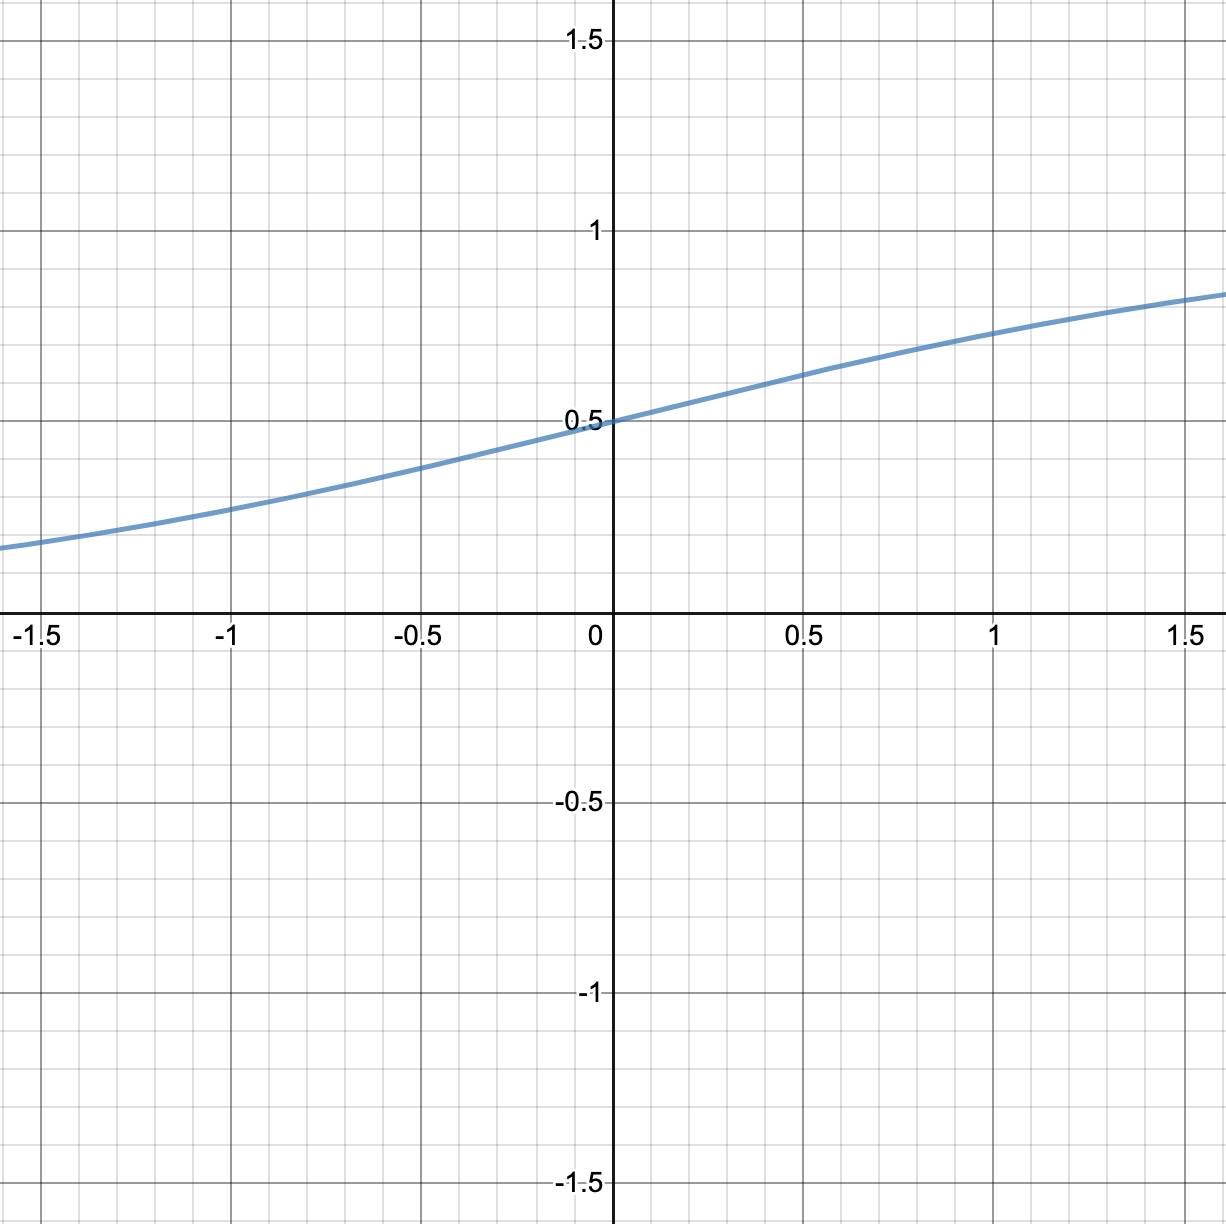
\includegraphics[width=\linewidth]{../figures/sigmoid.png}
		\caption{\texttt{Sigmoid}}
		\label{sigmoid}
	\end{subfigure}
\caption{Funzioni di attivazione utilizzate. La funzione sigmoidea rappresentata in figura~\ref{sigmoid} è definita come: $P(t)=\frac{1}{1+e^{-t}}$.}
\label{act_fun}
\end{figure}


        %%%%%%%%%%%%%%%%%%%  CAPITOLO 3.2.2  %%%%%%%%%%%%%%%%%%%

\subsection{Pre Training}\label{pre_training}
In fase di pre-training ho effetuato due operazioni: la normalizzazione dei dati e lo split del dataset in un \texttt{training\_set} ed un \texttt{validation\_set}. Ho inoltre effettuato un test per la verifica della convergenza della rete.


Gli output sono stati normalizzati in modo da appartenere all'intervallo $[0, 1]$, nel caso di \textit{Sigmoid} come funzione di attivazione, oppure a $[-1, 1]$ nel caso di \textit{Tanh}. Le formule utilizzate per la normalizzazione nei due casi sono:
\begin{equation}\label{norm1}
y'=\frac{y+y_m}{y_m-y_M}
\end{equation}
\begin{equation}\label{norm2}
y'=\frac{2y-y_m-y_M}{y_M-y_m}
\end{equation}
dove $y_m$ corrisponde al minimo valore del parametro mentre $y_M$ corrisponde al massimo.
L'equazione~\ref{norm1} permette una normalizzazione dell'output in $[0, 1]$ mentre la~\ref{norm2} in $[-1, 1]$\footnote{Dopo aver effettuato il training e aver ottenuto i risultati, i dati sono stati rinormalizzati in modo da tornare al range iniziale.}.

Come nel caso dell'interpolazione, a partire dal dataset in Fig.~\ref{dataset} sono stati creati due subsets per poter effettuare separatamente il training della rete e la verifica della bontà delle sue previsioni. Circa il $75\%$ (126) degli elementi totali (169) costituisce il \texttt{training\_set} mentre il restante $25\%$ (43) costituische il \texttt{validation\_set}. Questa operazione di caricamento è stata fatta tramite un metodo messo a disposizione da \textit{PyTorch}, \texttt{DataLoader}, attraverso il seguente codice:
\insertcode{../scripts/loader.py}{Loader}\label{loader}
La scelta degli elementi che vanno a finire in un determinato subset è fatta casualmente grazie a \texttt{suffle = True}.


Una volta definita l'architettura di rete ed effettuate le operazioni di pre-training è necessario verificare la convergenza della rete, per essere certi che non vada in overfitting. Questo è stato fatto per ogni parametro e per ogni architettura.
Per effettuare il test della rete ho utilizzato un metodo di validazione chiamato \textbf{K-Fold}. Il metodo consiste in:
\begin{itemize}
	\item mescolare il dataset iniziale;
	\item sezionare il dataset attraverso $K suddivisioni$ di eguale numerosità. Nel mio caso $K=5$;
	\item utilizzare $K-1$ parti per il \texttt{training\_set} e la parte rimanente per il \texttt{validation\_set};
	\item valutare la \textit{loss function} relativa al training e al validation;
	\item ripetere l'operazione per $K$ volte usando a ogni iterazione una delle K parti per il \texttt{validation\_set}, e le altre K-1 per il \texttt{training\_set}.
\end{itemize}

\begin{figure}[!ht]
\centering
	\begin{subfigure}{\textwidth}
	    \centering
	    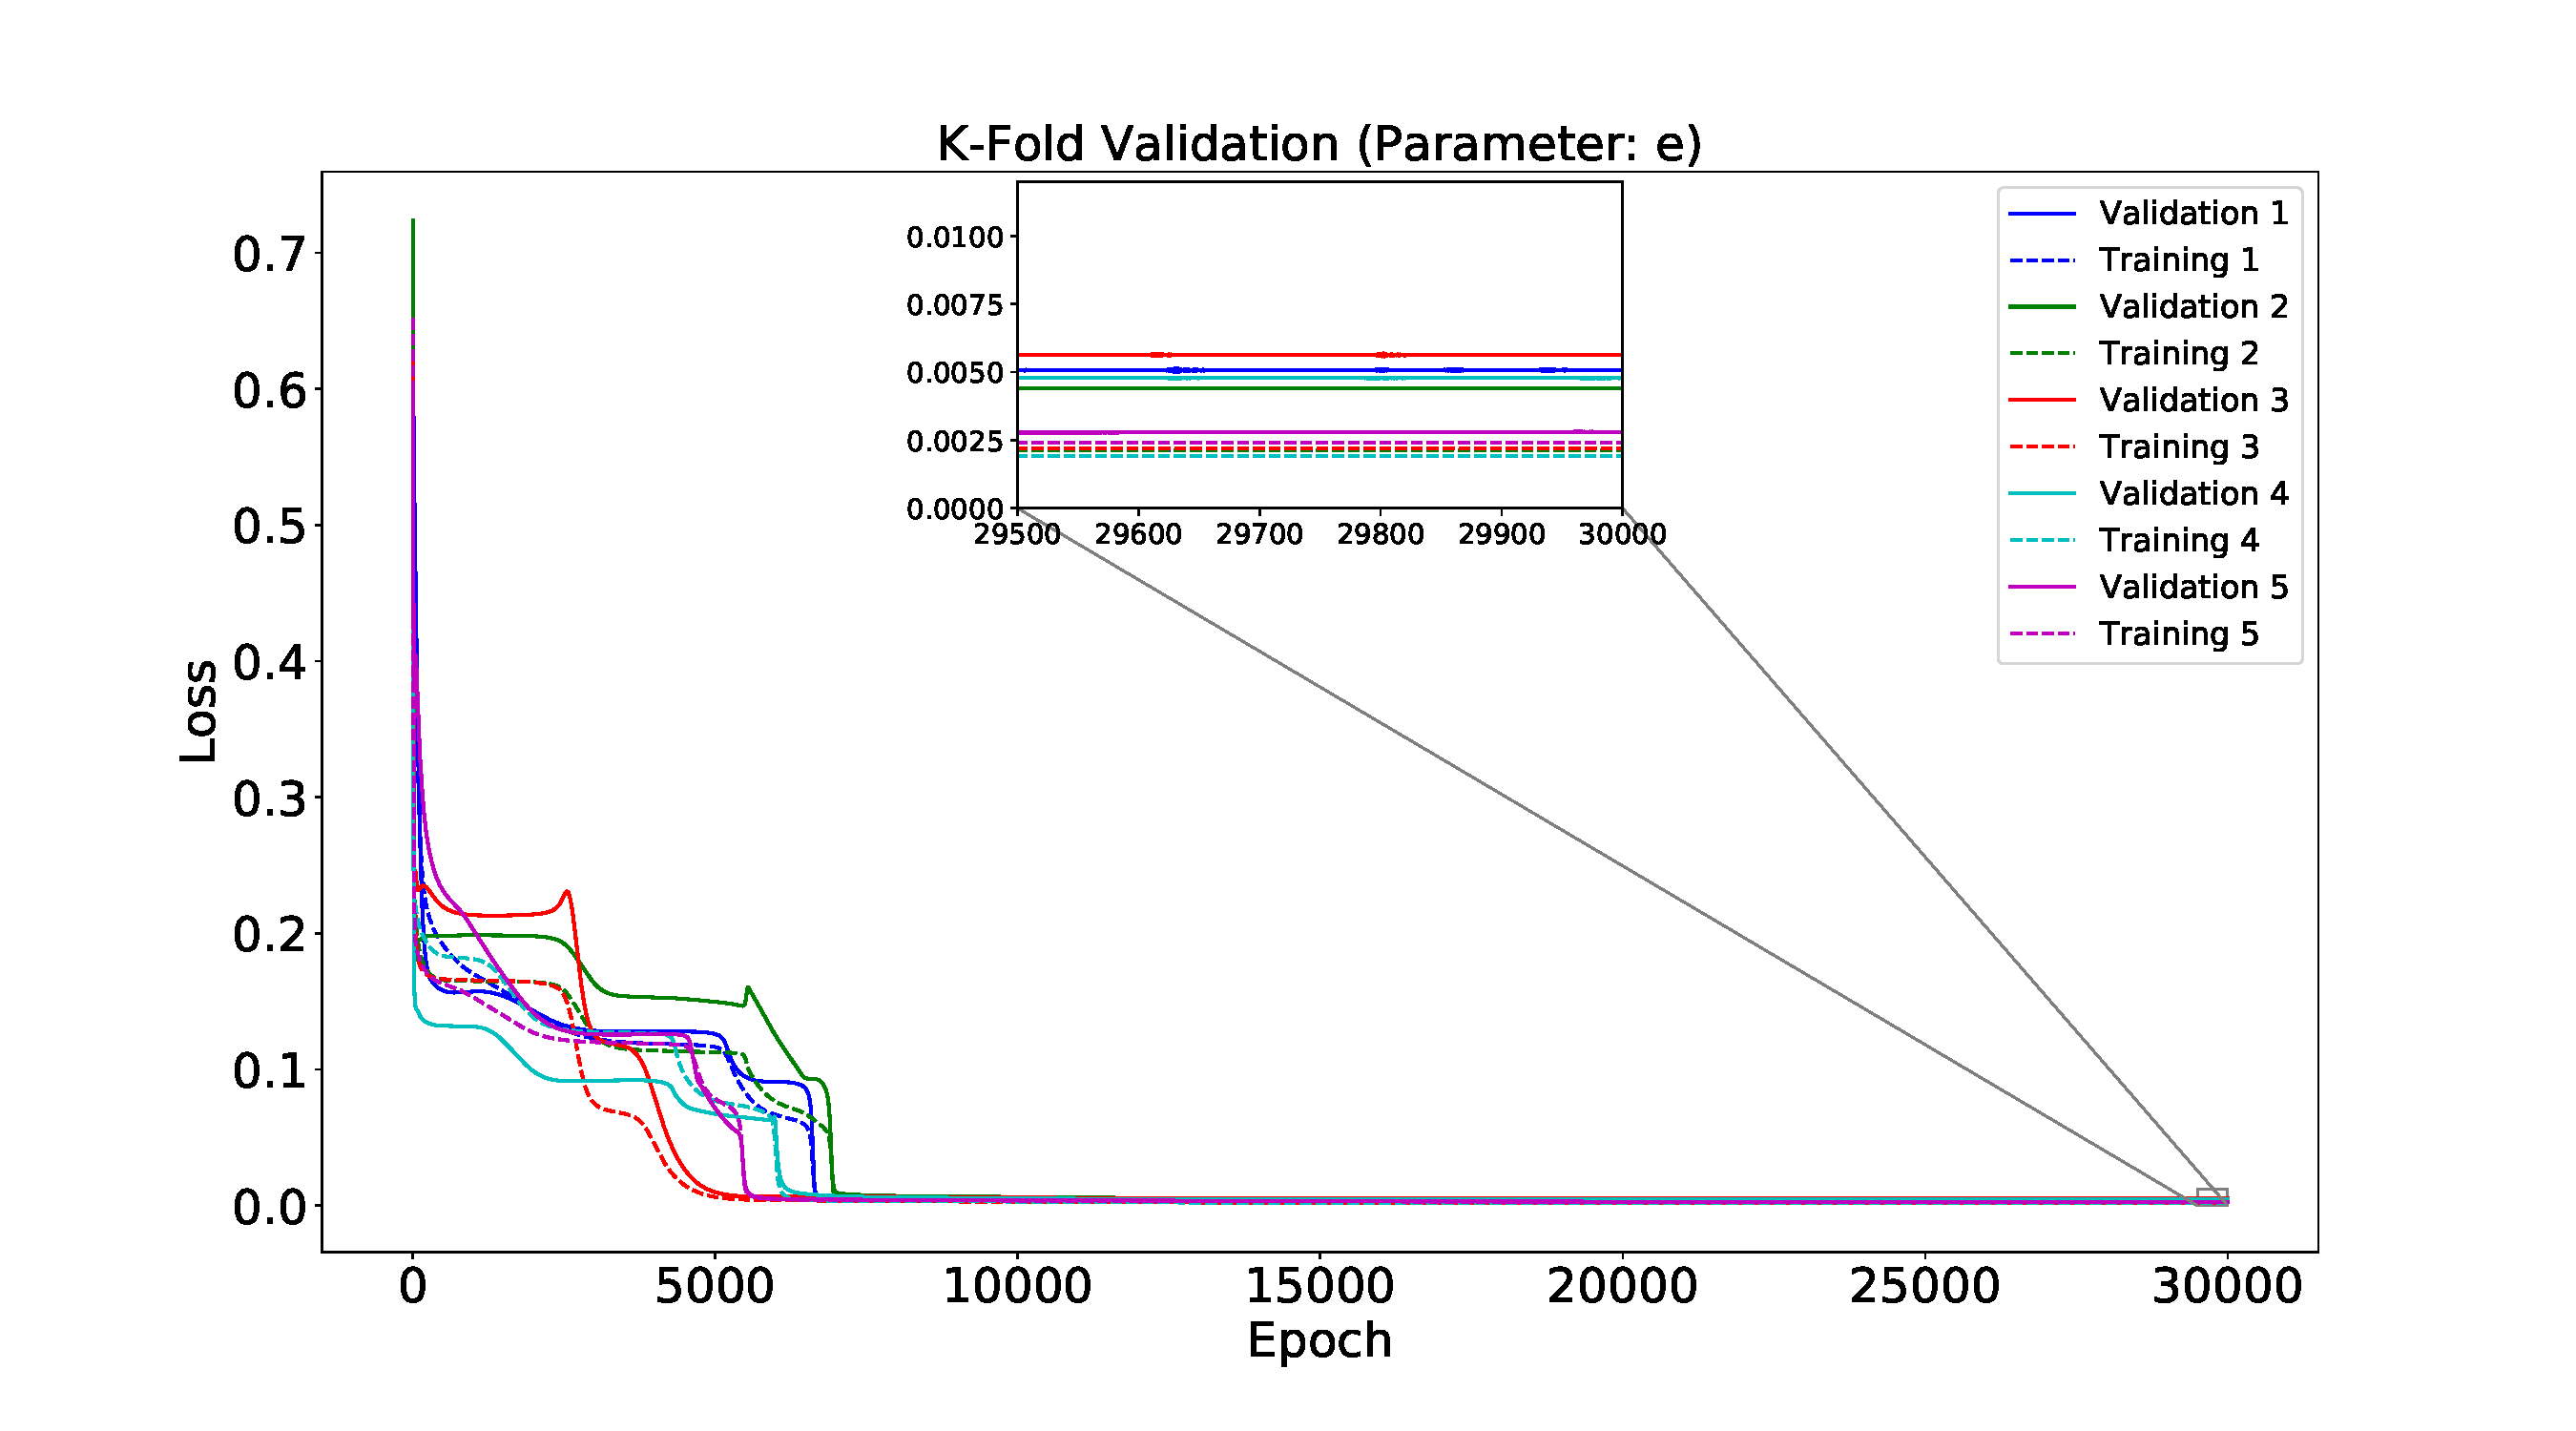
\includegraphics[width=0.77\linewidth]{../figures/validation_e_zoom.pdf}
	    \caption{Test di rete per il parametro \textit{e}. L'architettura di rete è data da 1 hidden layer e dalla $Tanh$ come funzione d'attivazione.}
	    \label{test1}
	\end{subfigure}
	\newline
	\begin{subfigure}{\textwidth}
		\centering
	    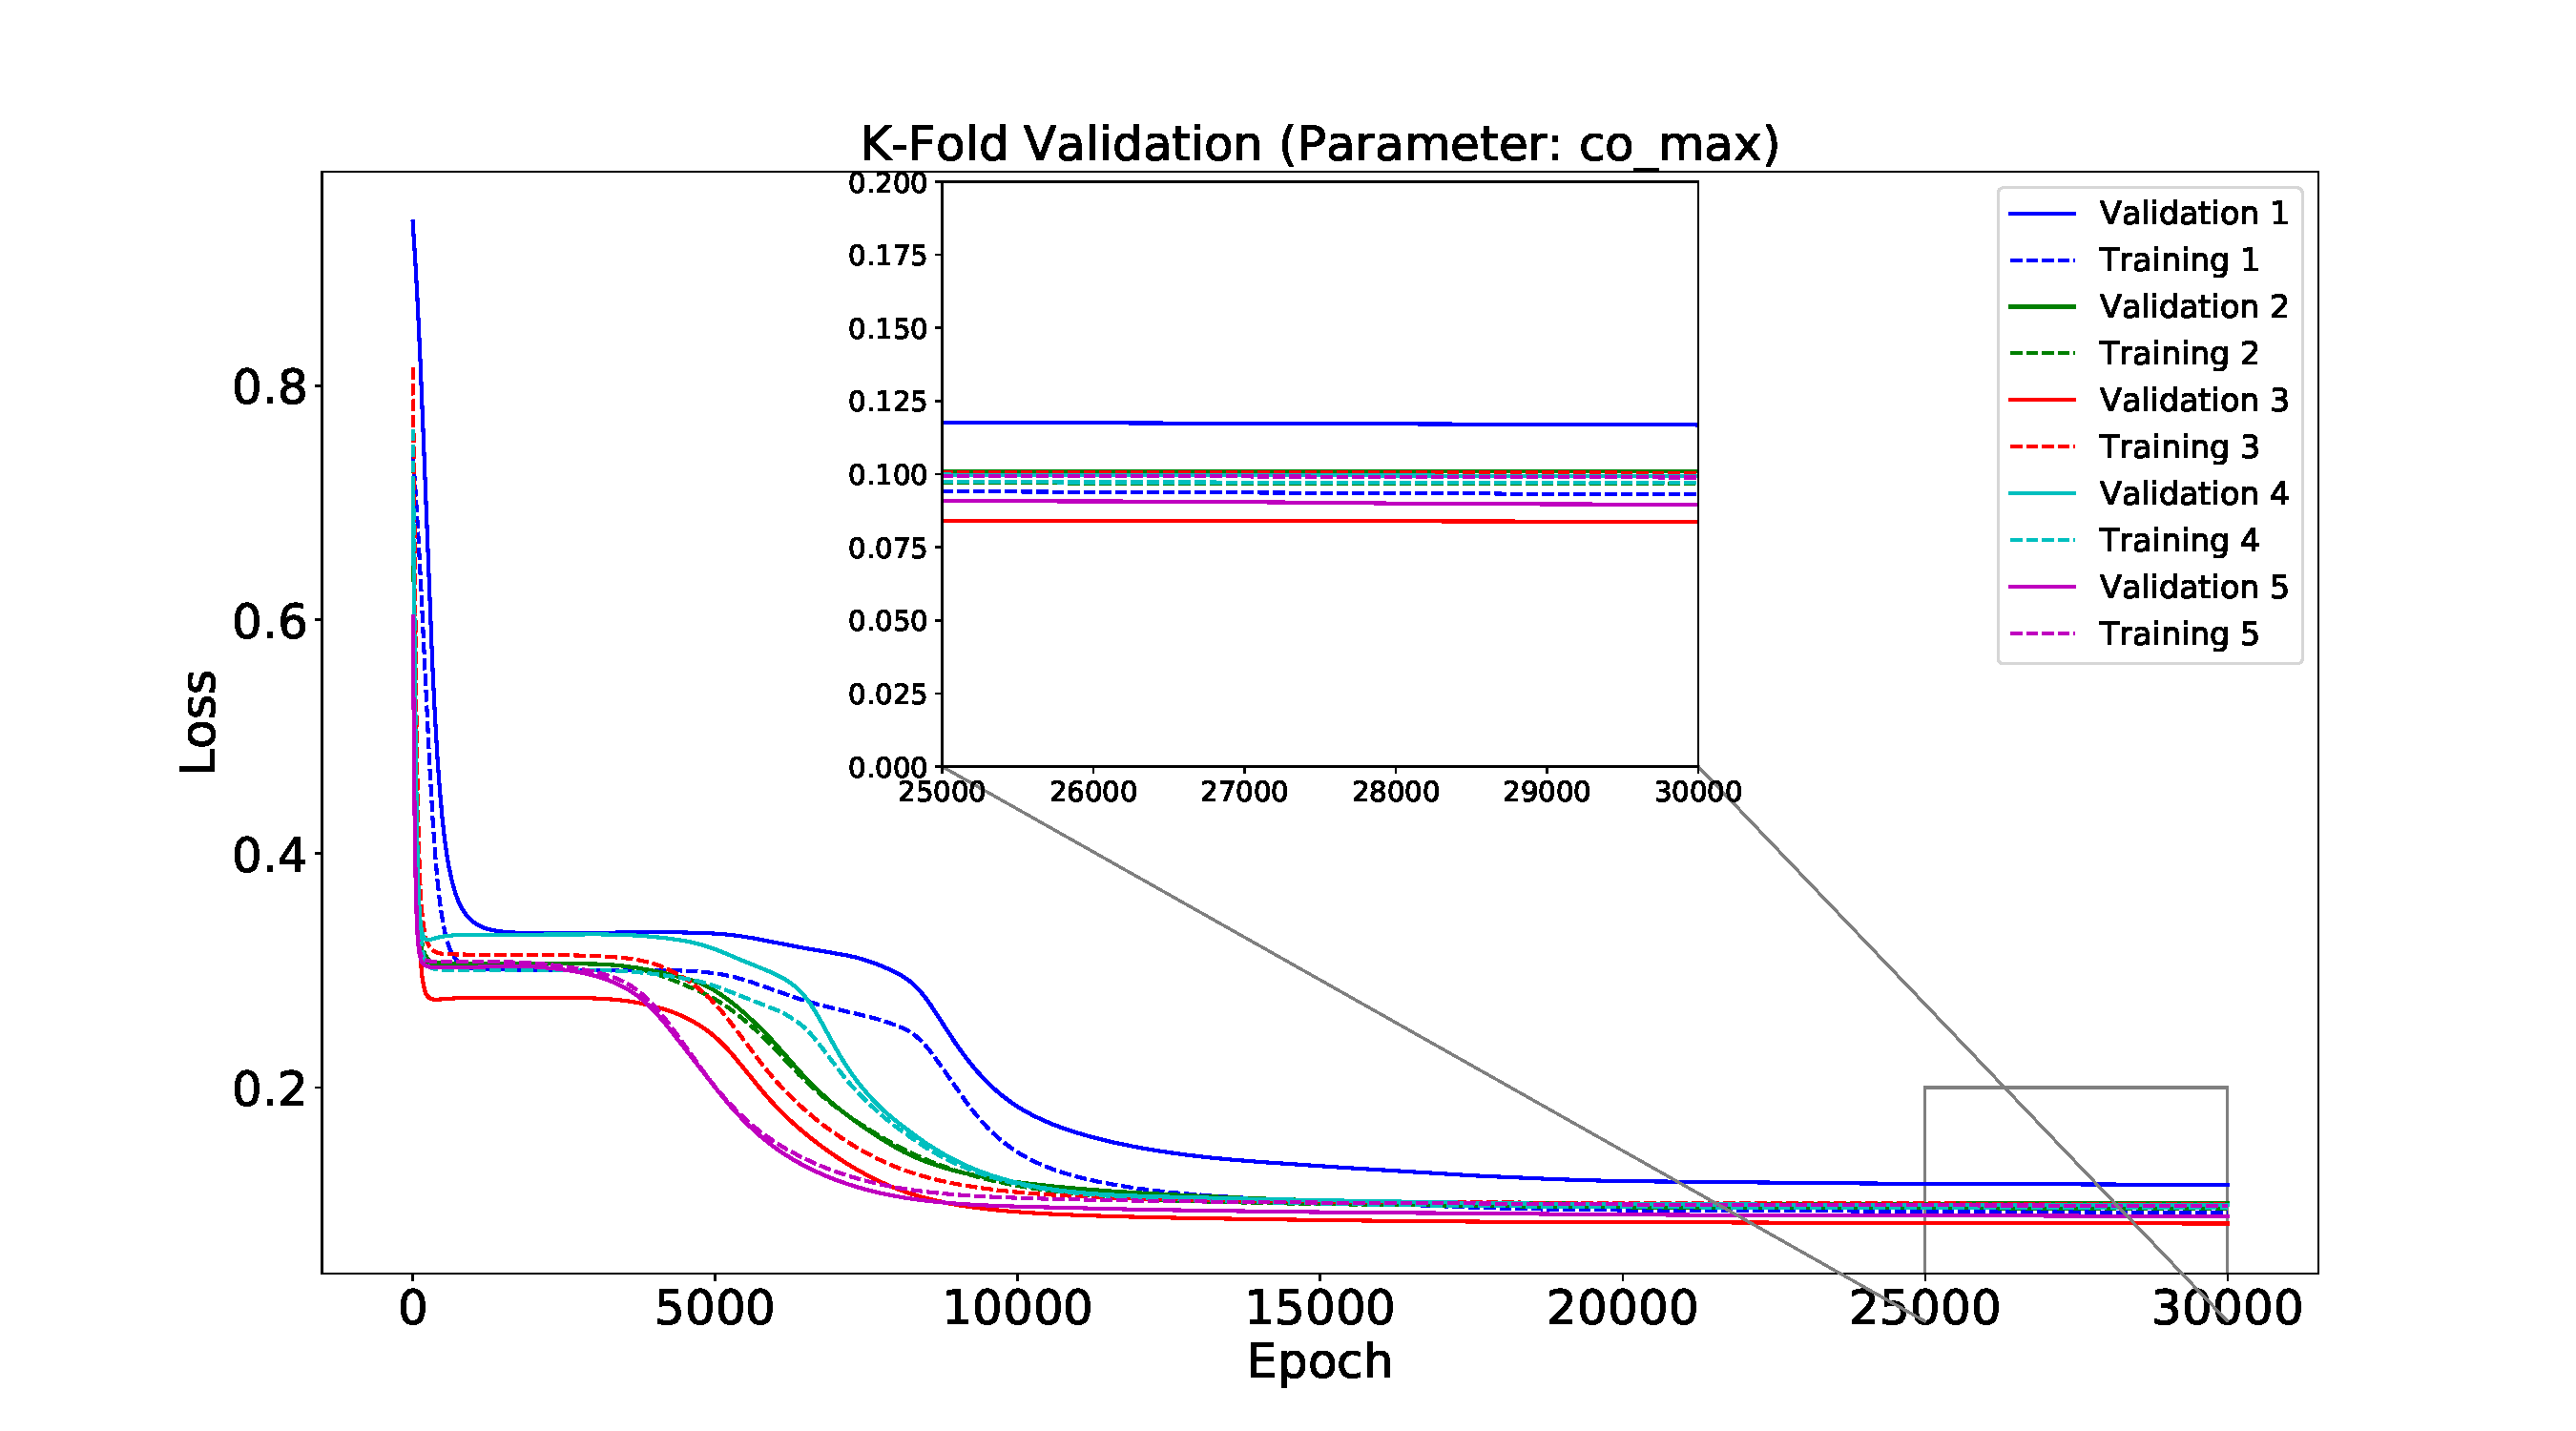
\includegraphics[width=0.77\linewidth]{../figures/validation_co_max_zoom.pdf}
		\caption{Test di rete per il parametro \textit{co\_max}. L'architettura di rete è data da 1 hidden layer e dalla $Sigmoid$ come funzione d'attivazione.}
		\label{test2}
	\end{subfigure}
	\caption{Test di rete per due diversi parametri e due diverse architetture. I grafici rappresenta il valore di \textit{loss} per il training e il validation; Nel caso ~\ref{test1} le curve tendono a 0 ma, come si nota dallo zoom-in, non valgono esattamente 0. Nel caso ~\ref{test2} invece non viene raggiunto un buon valore di \textit{loss}, quella particolare architettura non sarà quindi ottimale per il parametro \textit{co\_max}. Grafici di questo tipo ci mostrano che le reti non vanno in overfitting perché, se così fosse, le curve relative al validation dovrebbero crescere all'aumentare delle epoche.}
	\label{test_rete}
\end{figure}

In Fig.~\ref{test_rete} sono rappresentati alcuni dei risultati ottenuti.


        %%%%%%%%%%%%%%%%%%%  CAPITOLO 3.2.3  %%%%%%%%%%%%%%%%%%%

\subsection{Training}\label{training}
Per effettuare il training ho innanzitutto creato una funzione che mi permettesse di inizializzare i pesi della rete. Questo è stato fatto poiché essi vengono inizializzati da Pytorch casualmente ed è quindi necessario avere a disposizione una funzione apposita che sia in grado di determinare la distribuzione dei loro valori iniziali. Con la giusta inizializzazione è più probabile che la rete converga.
\insertcode{../scripts/init_weights.py}{Inizializzazione di weights e biases}\label{init_weights}
Com'è possibile osservare dal codice~\ref{init_weights}, i biases di rete sono inizializzati a $0$ mentre i weights sono distribuiti uniformemente tra $0$ e $1$.


Dopo aver inizializzato i pesi ho caricato i dataset per il training e per il validation attraverso il codice~\ref{loader}.
Il training è stato effettuato su 30000 epoche. Il numero è elevato ma, avendo provato tramite la fase di validazione, spiegata in dettaglio nella Sez.~\ref{pre_training}, che la rete non va in overfitting ho deciso di mantenerlo. 
Inoltre ogni 5000 epoche ho rieffettuato uno \textit{shuffle} del \texttt{training\_set} e del \texttt{validation\_set}, sempre attraverso il codice~\ref{loader}. Questa tecnica, chiamata di \textit{shuffling}, è utilizzata per minimizzare i problemi di overfitting e permette di rendere più robusto il processo di convergenza.


Nella prossima sezione verranno presentati i risultati ottenuti e confrontati con quelli relativi all'interpolazione.

        %%%%%%%%%%%%%%%%%%%  CAPITOLO 3.2.4  %%%%%%%%%%%%%%%%%%%

\section{Confronto dei risultati}\label{risultati}
Prima di presentare i risultati ottenuti riassumo le analisi che ho effettuato. I parametri presi in considerazione sono 5: ellitticità, FWHM (rispetto a x), FWHM (rispetto a y), componente co-polare massima e componente cross-polare massima. Le reti costruite sono 6 e gli elementi che ne caratterizzano l'architettura sono riportati in Tab.~\ref{architetture}. In totale ho quindi effettuato 30 analisi.
Per ogni analisi ho prodotto due grafici che confrontano i risultati ottenuti tramite le  reti neurali e tramite l'interpolazione. Infine ho creato dei \textit{violin plots} che mi permettessero, in un unico grafico, di comparare i due metodi al variare delle arichitetture.


Il grafico riportato in Fig.~\ref{hist_good} è rappresentativo del caso in cui le reti neurali predicono il valore del parametro in maniera più efficace rispetto all'interpolazione, mentre quello riportato in Fig.~\ref{hist_bad} mostra che nessuno dei due approcci è apprezzabilmente più efficace dell'altro.

\begin{figure}[!ht]
	\centering
	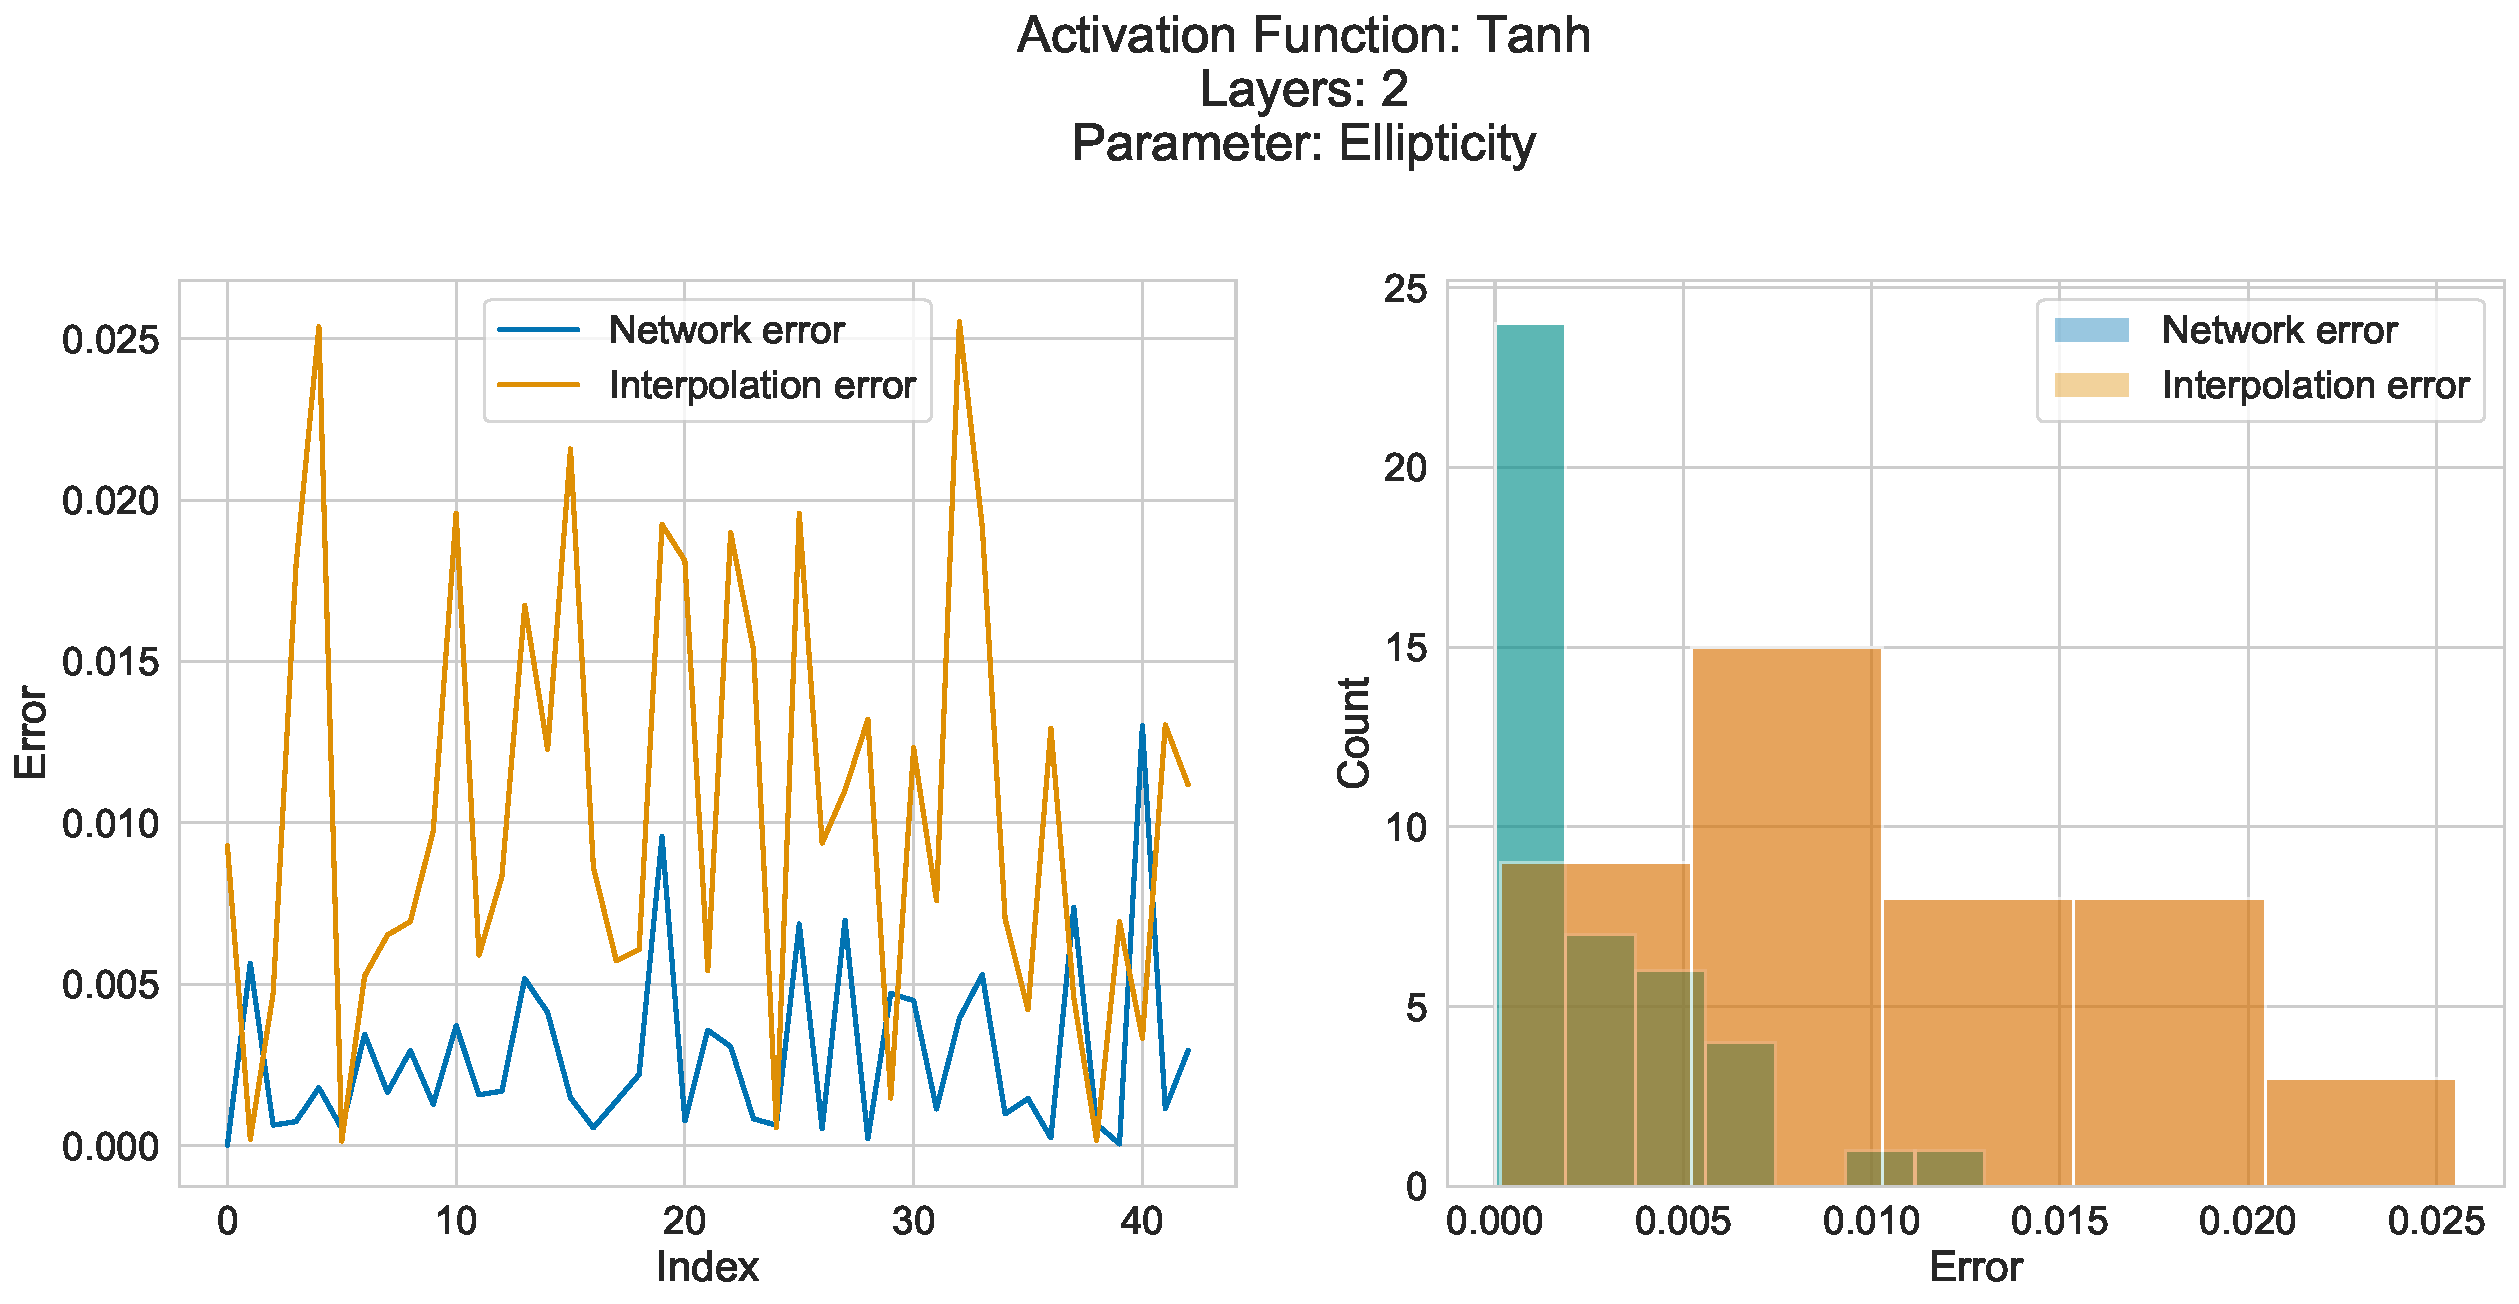
\includegraphics[width=\linewidth]{../figures/hist_good.pdf}
	\caption{Sulla sinistra è rappresentato il confronto dell'errore tra valore vero e valore stimato tramite il metodo di interpolazione, in arancione, e tramite la rete neurale, in blu. Sulla destra è rappresentato lo stesso grafico sotto forma di istogramma. Il parametro analizzato è l'ellitticità e l'architettura della rete è data da due hidden layers e dalla Tanh come funzione d'attivazione.}
	\label{hist_good}
\end{figure}
\vspace{1cm}
\begin{figure}[!ht]
	\centering
	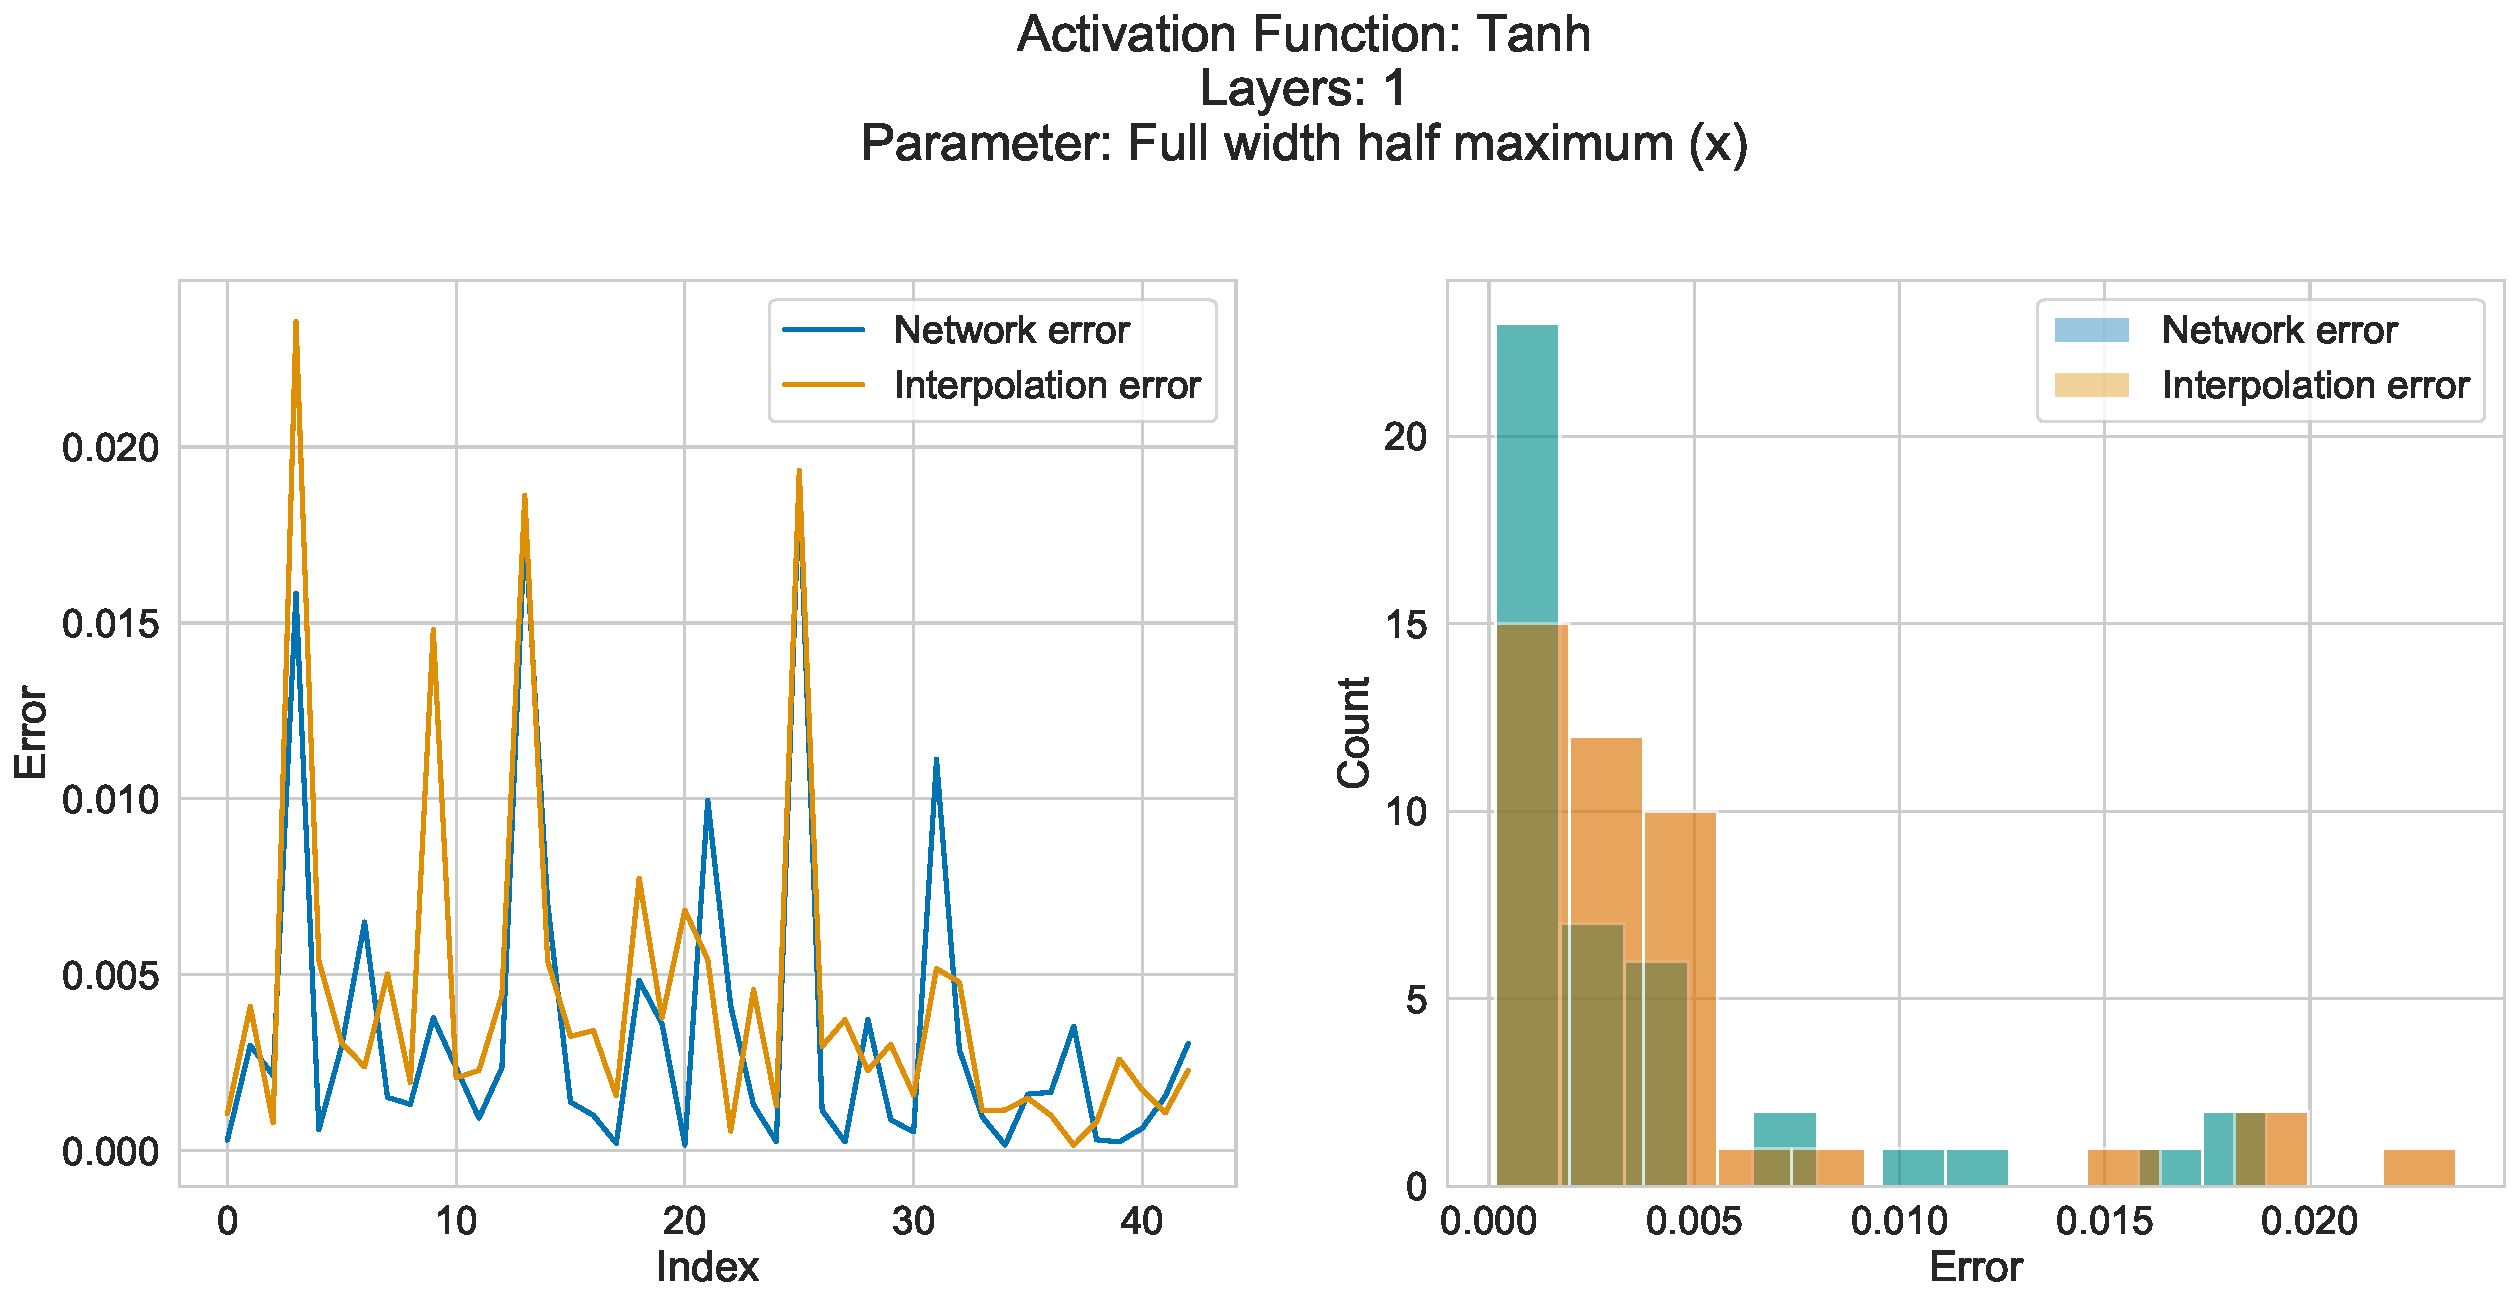
\includegraphics[width=\linewidth]{../figures/hist_bad.pdf}
	\caption{Il significato del grafico è lo stesso di~\ref{hist_good} ma in questo caso il parametro analizzato è la FWHM rispetto a $x$ e l'architettura della rete è data da un solo hidden layer dalla Tanh come funzione d'attivazione. Il valore dell'errore è espresso in gradi.}
	\label{hist_bad}
\end{figure}

\newpage
I \textit{violin plots} permettono di visualizzare la densità di probabilità di ottenere un determinato valore dell'errore. Tanto più è piccata la curva per valori bassi dell'errore, quanto più il risultato è buono.

\vspace{3cm}
\begin{figure}[!ht]
	\begin{subfigure}{\textwidth}
	    \centering
	    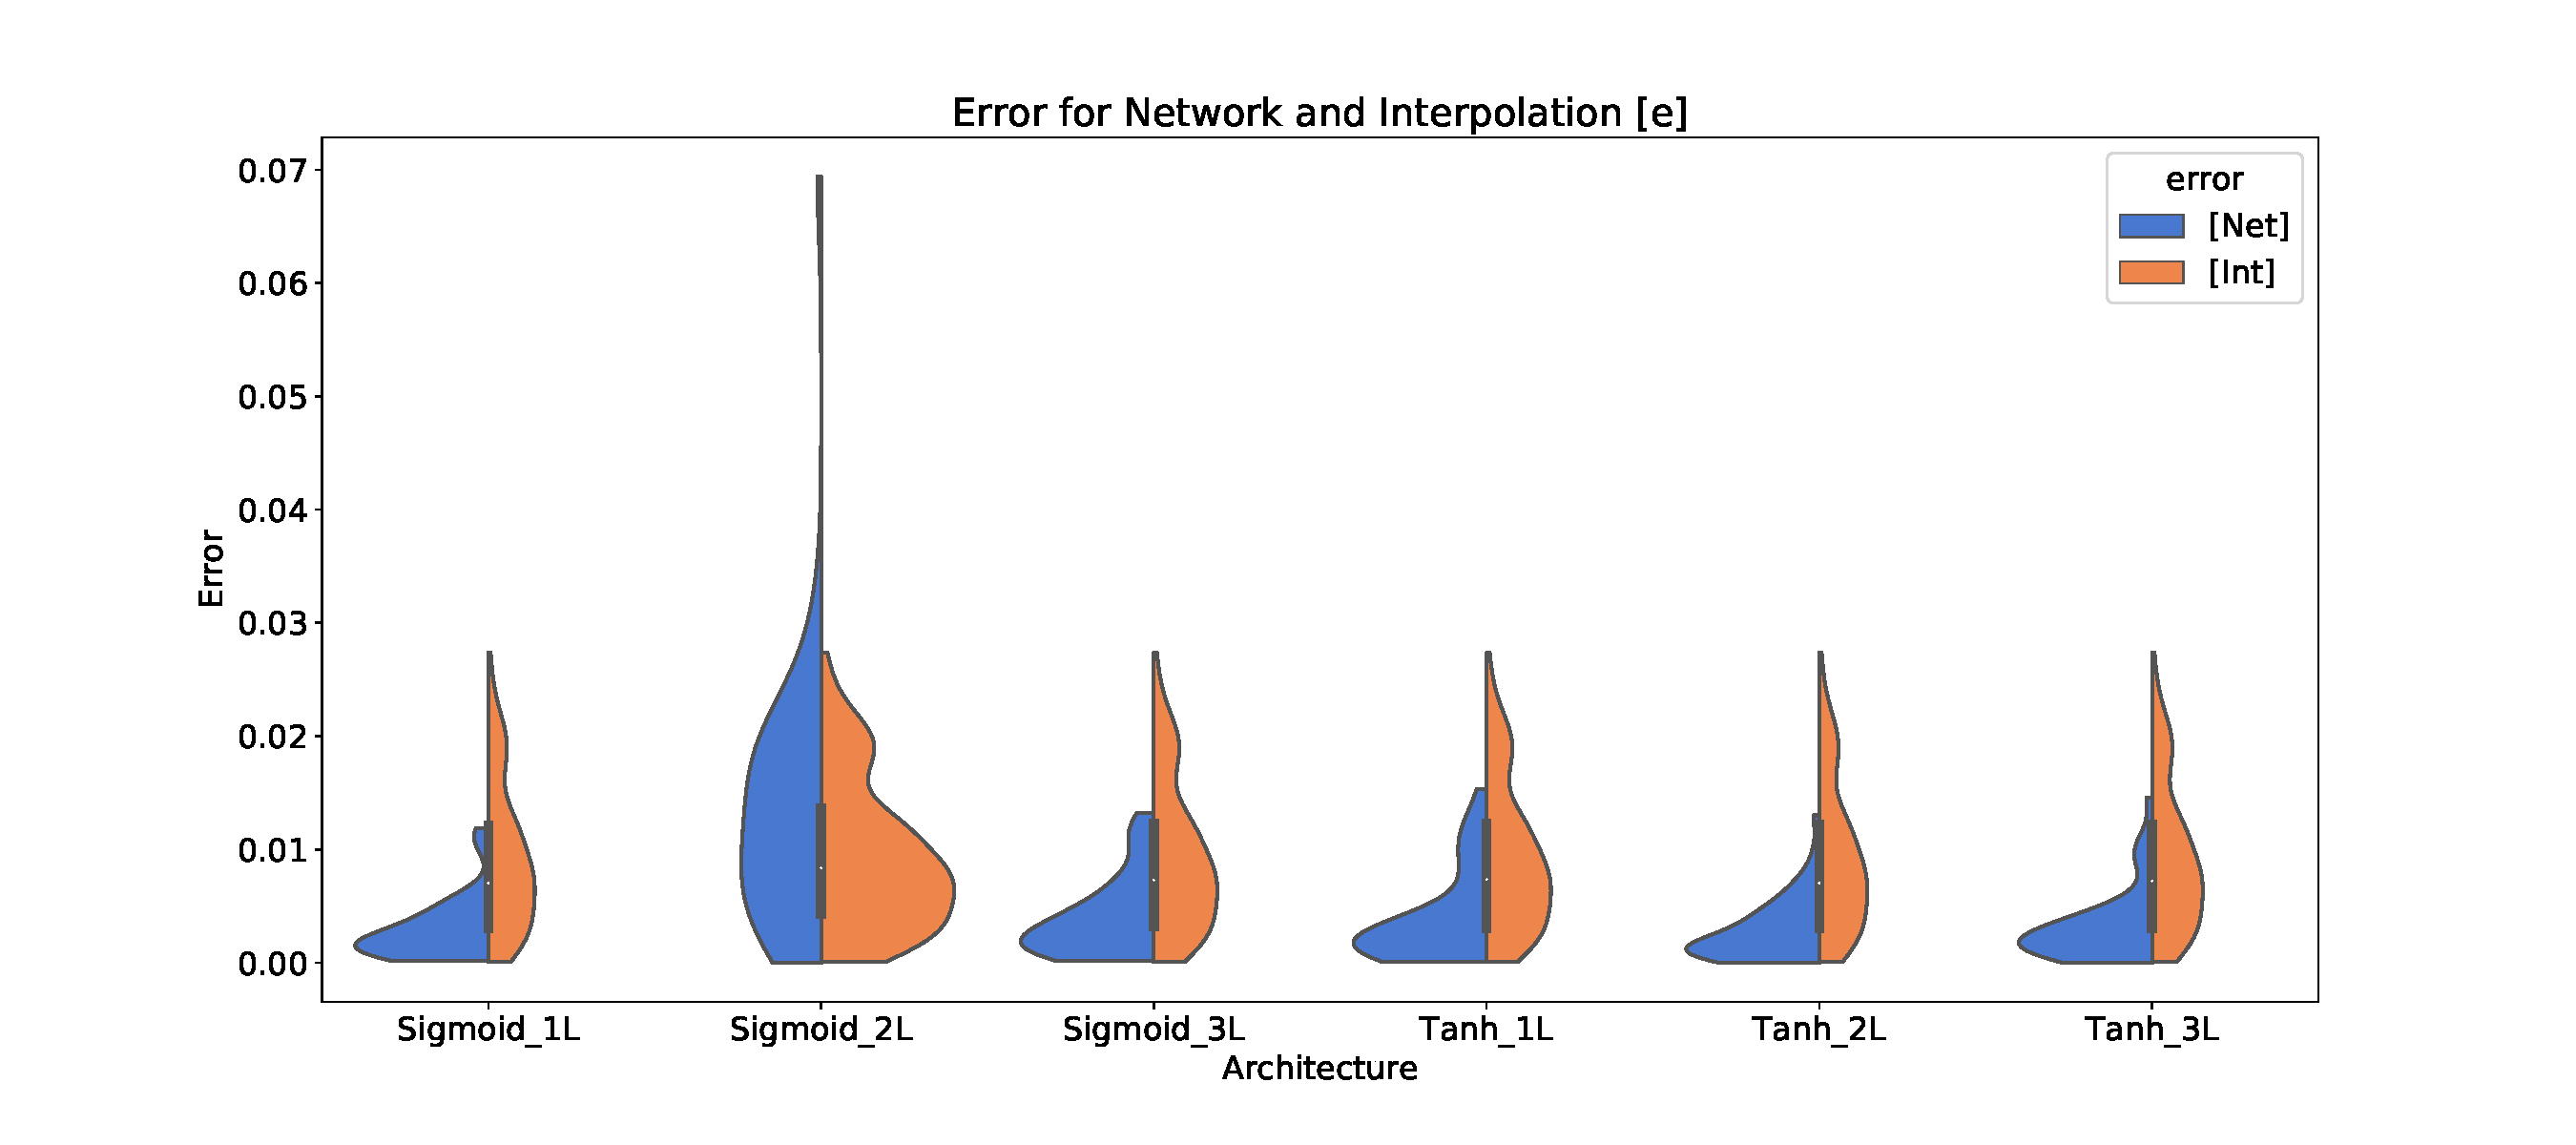
\includegraphics[width=\linewidth]{../figures/violin_plot_e.pdf}
	    \caption{Violin plot per l'ellitticità.}
	    \label{violin_e}
	\end{subfigure}
	\newline
	\newline
	\newline
	\newline
	\begin{subfigure}{\textwidth}
	    \centering
	    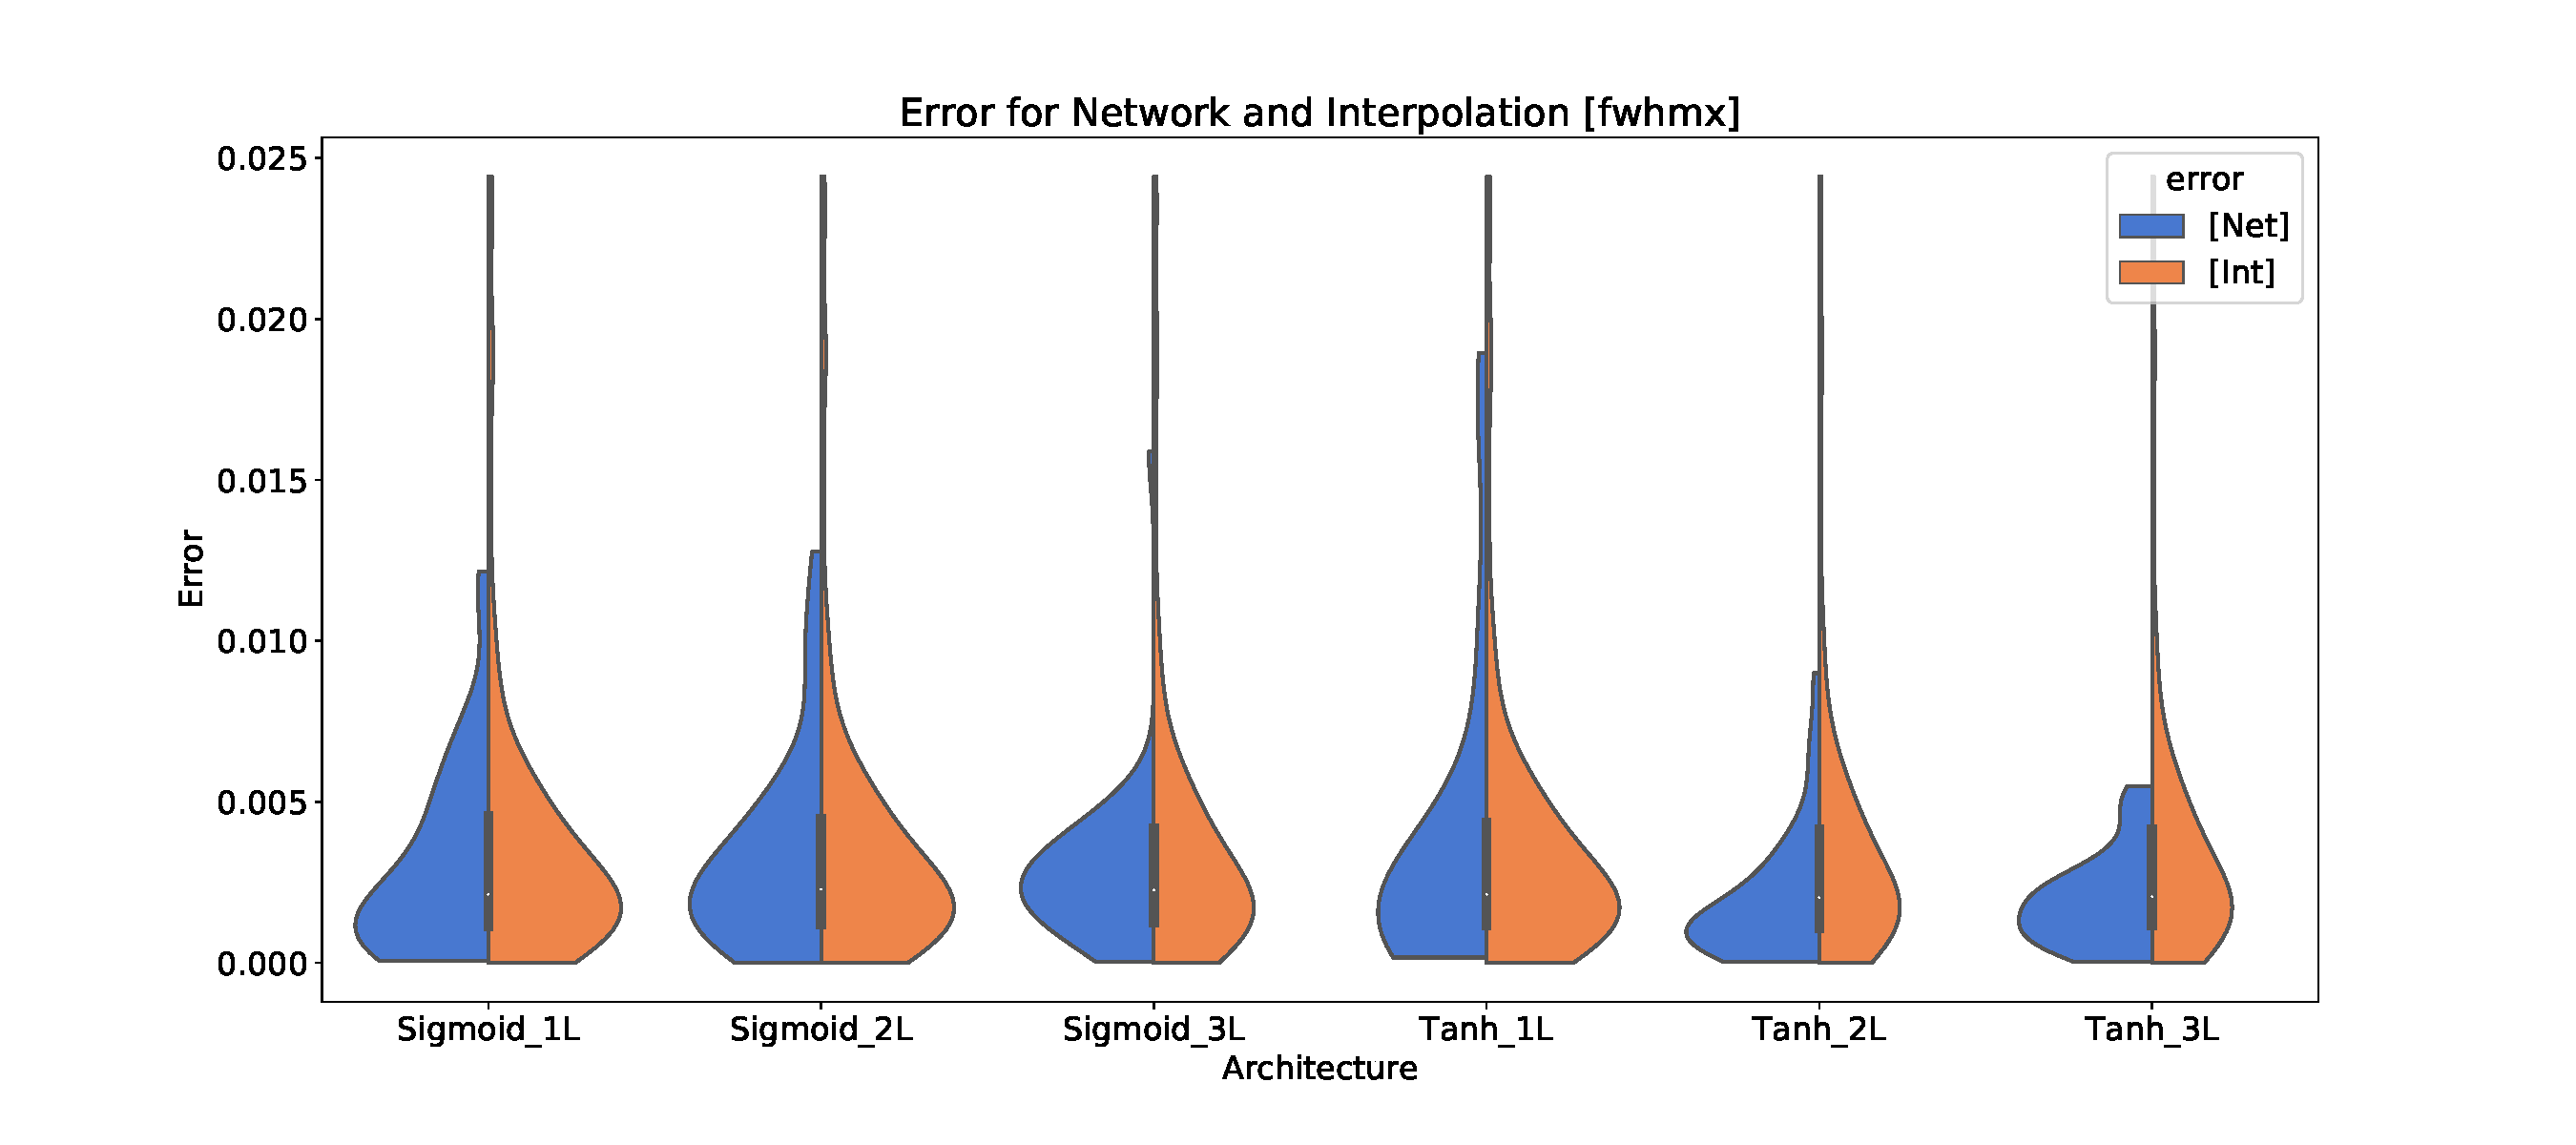
\includegraphics[width=\linewidth]{../figures/violin_plot_fwhmx.pdf}
	    \caption{Violin plot per la fwhm(x). L'errore è espresso in gradi.}
	    \label{violin_fwhmx}
	\end{subfigure}
\end{figure}
\newpage
\begin{figure}[!ht]\ContinuedFloat
	\vspace{4cm}
	\begin{subfigure}{\textwidth}
		\centering
		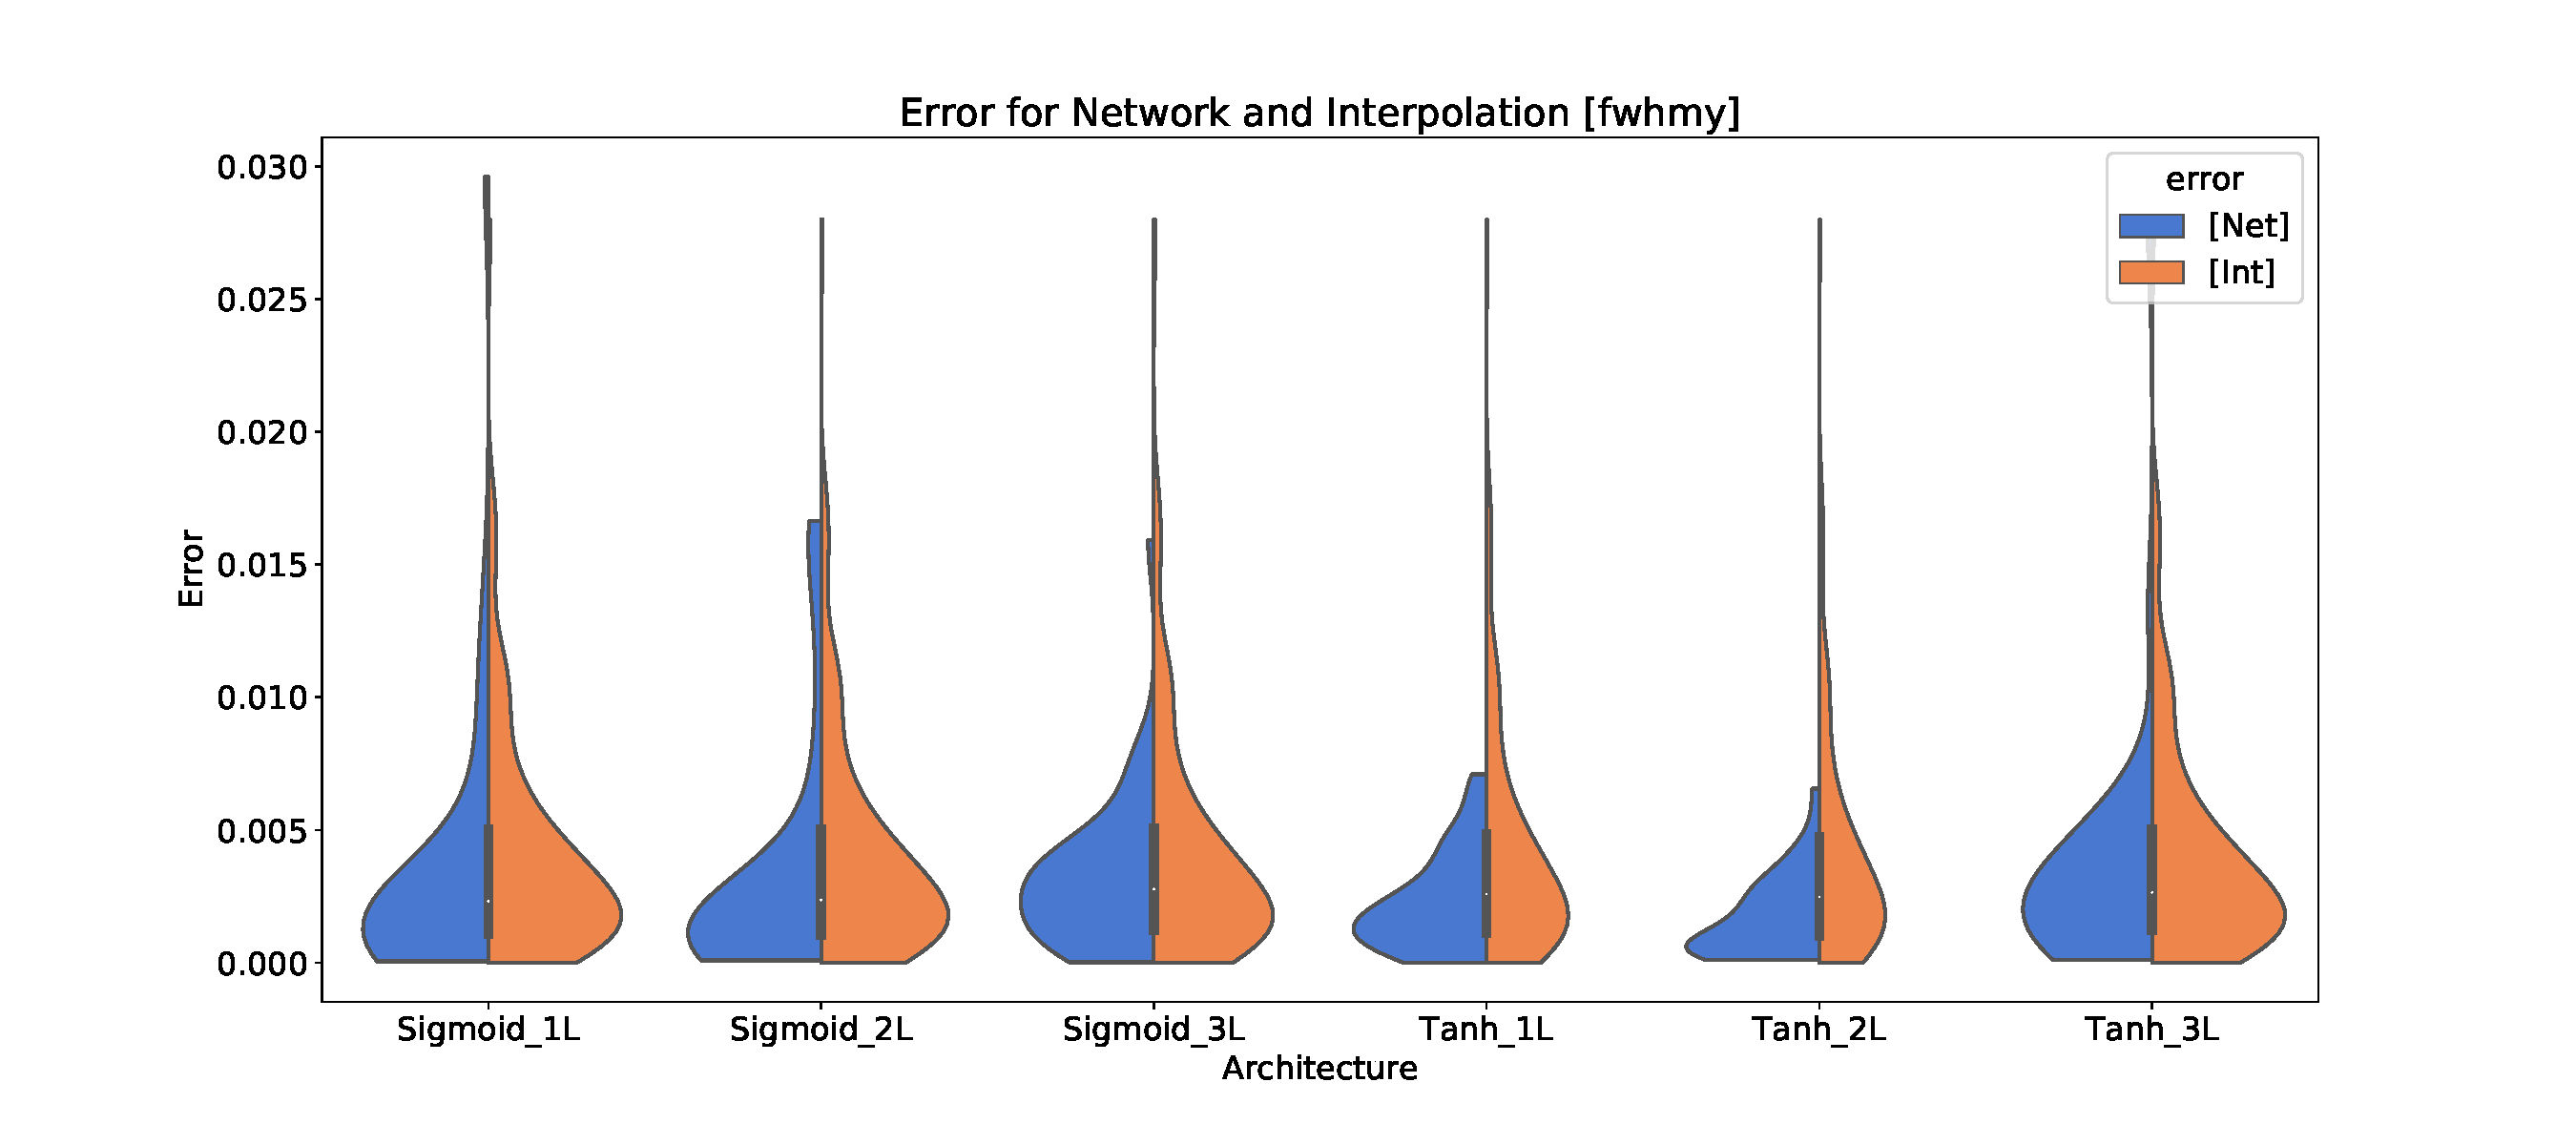
\includegraphics[width=\linewidth]{../figures/violin_plot_fwhmy.pdf}
		\caption{Violin plot per la fwhm(y). L'errore è espresso in gradi.}
		\label{violin_fwhmy}
	\end{subfigure}
	\newline
	\newline
	\newline
	\newline
	\begin{subfigure}{\textwidth}
	    \centering
	    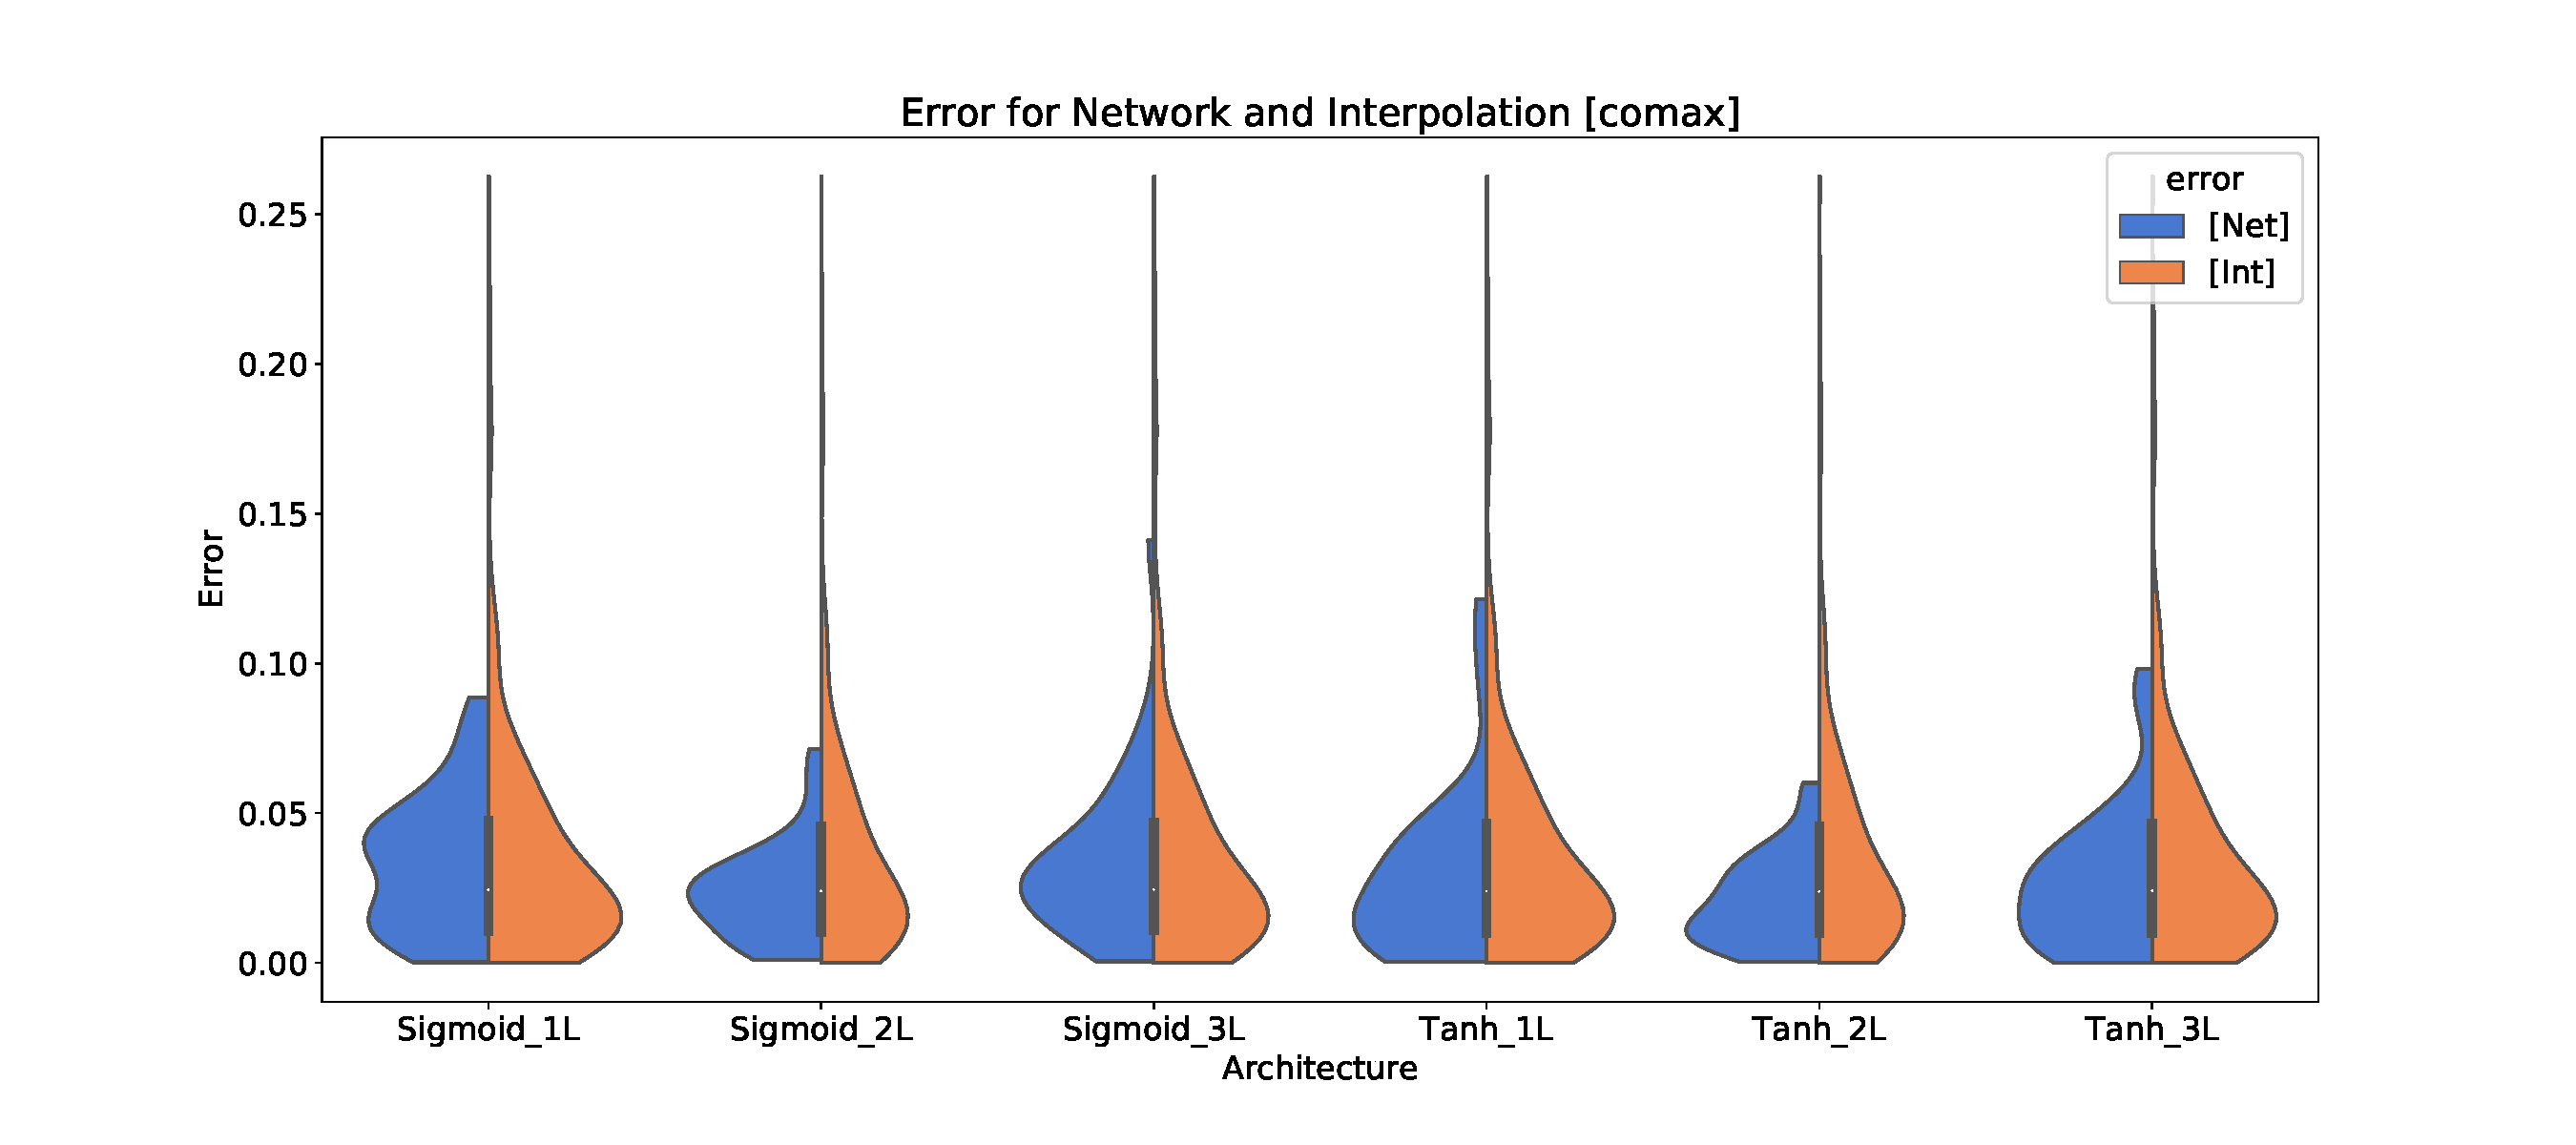
\includegraphics[width=\linewidth]{../figures/violin_plot_comax.pdf}
	    \caption{Violin plot per la componente co-polare massima. L'errore è espresso in $dBi$.\footnote{Il $dBi$ è il guadagno in decibel rispetto a un'antenna isotropa.}}
	    \label{violin_comax}
	\end{subfigure}
\end{figure}
\newpage
\begin{figure}[!t]\ContinuedFloat
	\begin{subfigure}{\textwidth}
		\centering
	    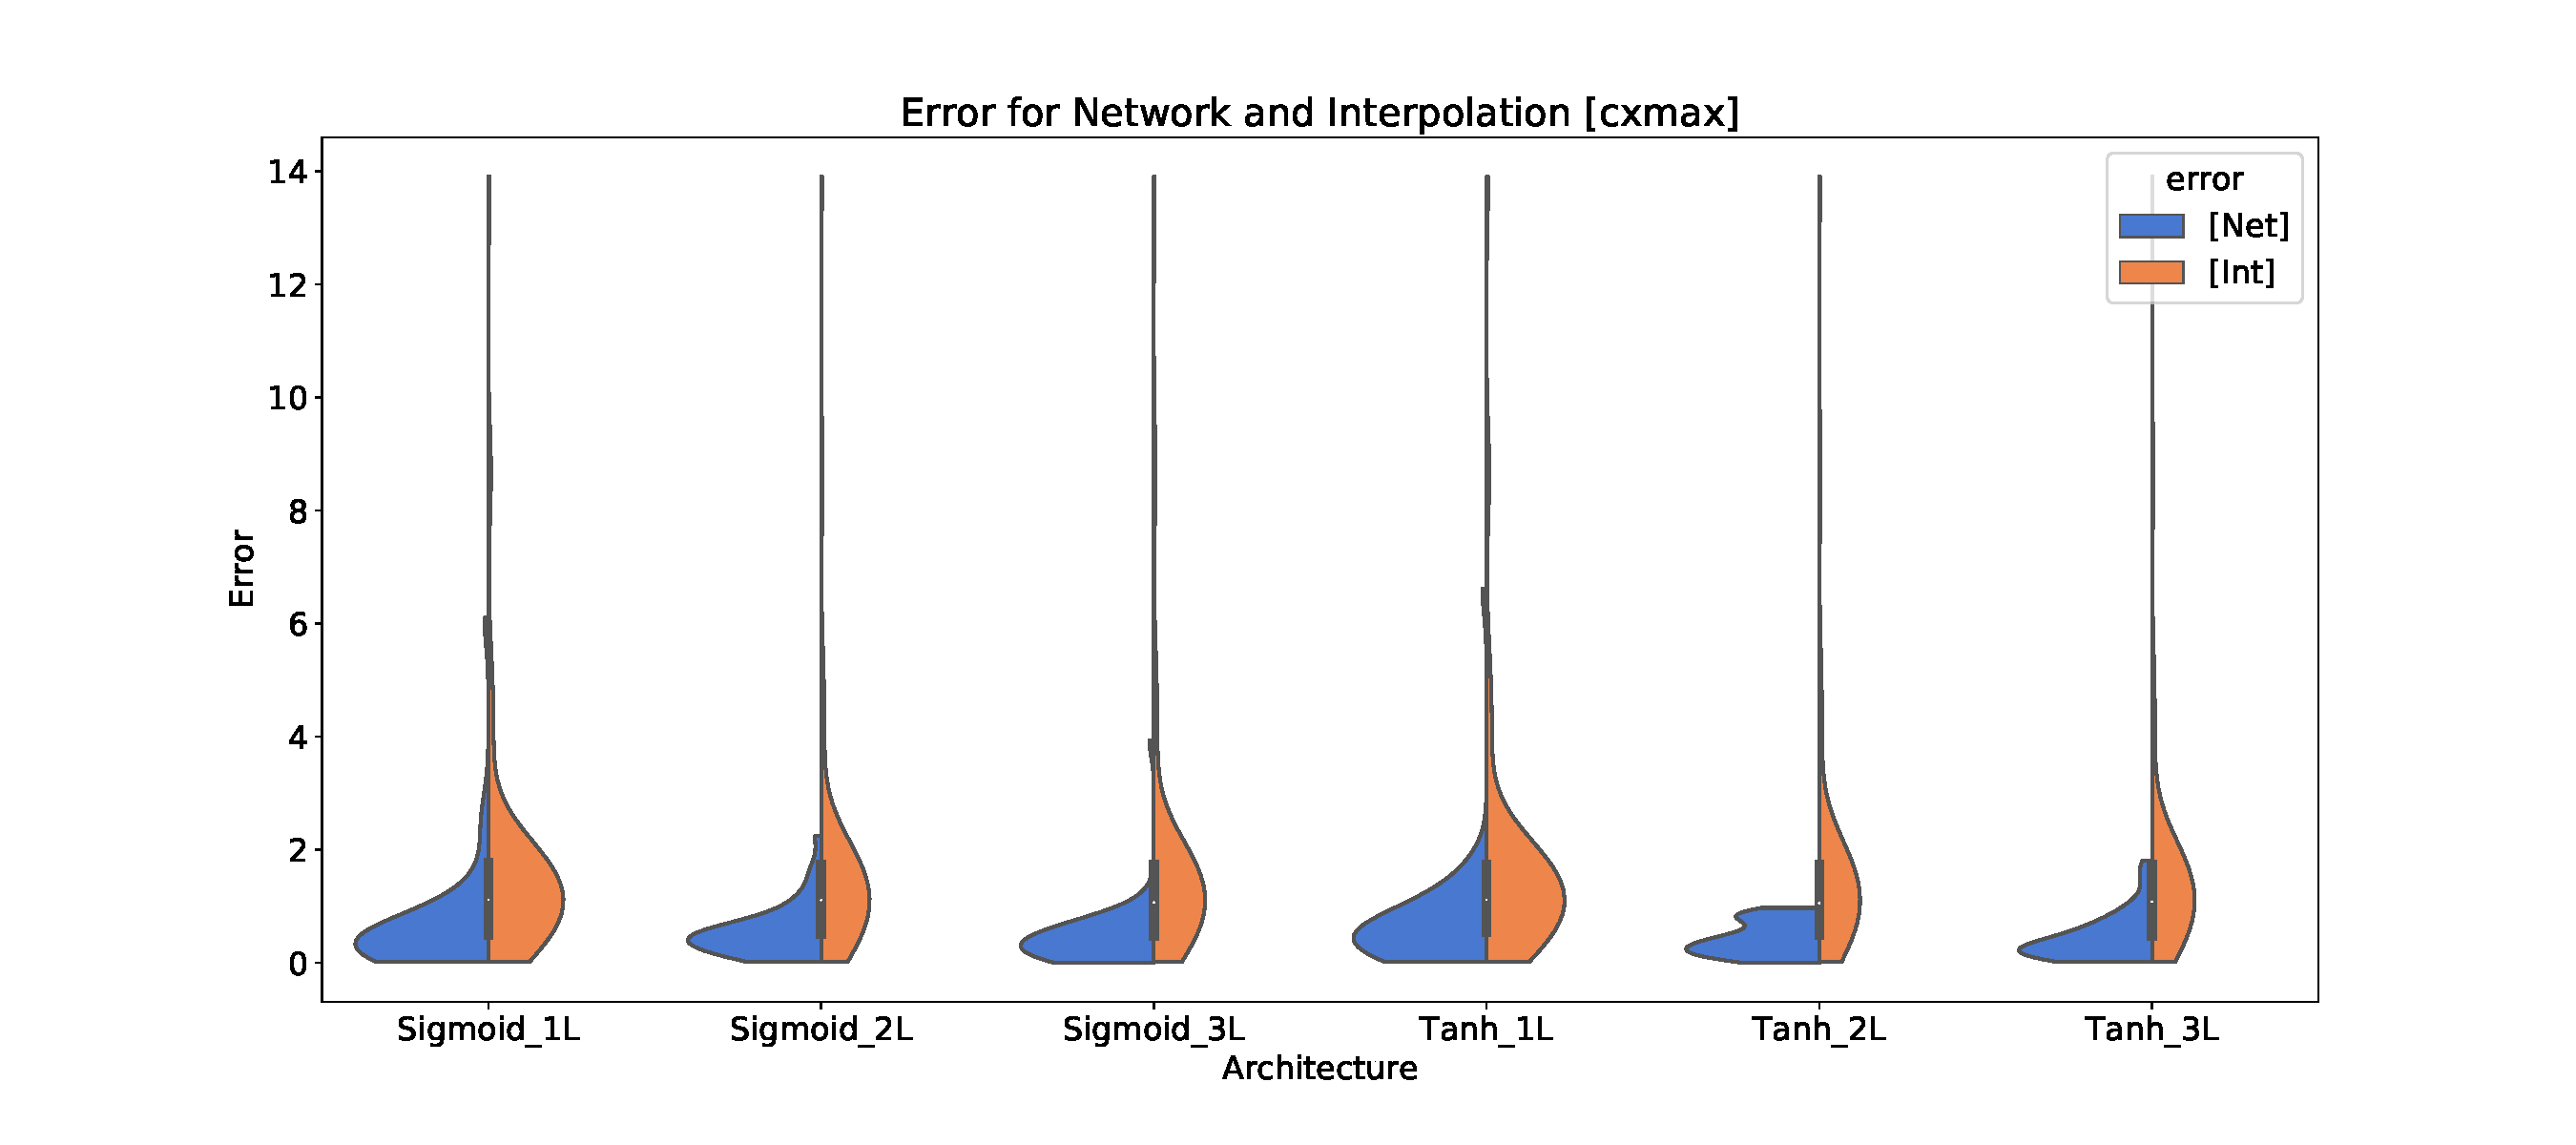
\includegraphics[width=\linewidth]{../figures/violin_plot_cxmax.pdf}
	    \caption{Violin plot per la componente cross-polare massima. L'errore è espresso in $dBi$.}
	    \label{violin_cxmax}
	\end{subfigure}
\end{figure}

\pagebreak
Questi grafici mostrano che per i parametri di ellitticità e componente cross-polare massima le reti neurali, con la giusta architettura\footnote{Per esempio, \textit{Tanh\_2L} per l'ellitticità o \textit{Tanh\_3L} per la componente cross-polare massima.}, forniscono risultati apprezzabilmente migliori rispetto a quelli ottenuti con l'interpolazione.
Per i due parametri di FWHM e per la componente co-polare massima i risultati delle reti risultano migliori solo per poche specifiche architetture.
In Tab.~\ref{stats} sono riportati i risultati numerici rappresentativi della bontà dei modelli.

%\makebox[\textwidth][c]{}



\begin{table}[!ht]
	%\centerfloat
	\centering
	\begin{adjustbox}{center}
	\begin{tabular}{|| c || c | c | c | c | c||}
	\hline
	& \textbf{Ellitticità} & \textbf{$\text{FWHM}_\text{x}$} & \textbf{$\text{FWHM}_\text{y}$} & \textbf{Co\_max} & \textbf{Cx\_max} \\
	\hline\hline\xrowht[()]{20pt}
	\textbf{Interpolation} & $0.0082_{-0.0039}^{+0.0045}$ & $0.0022_{-0.0010}^{+0.0023}$ & $0.0028_{-0.0015}^{+0.0026}$ & $0.0240_{-0.0139}^{+0.0240}$ & $1.2566_{-0.6049}^{+0.5671}$\\
	\hline\xrowht[()]{20pt}
	\textbf{Tanh\_1L} & $0.0026_{-0.0018}^{+0.0018}$ & $0.0016_{-0.0008}^{+0.0021}$ & $0.0017_{-0.0007}^{+0.0015}$ & $0.0230_{-0.0152}^{+0.0163}$ & $0.4951_{-0.2269}^{+0.2935}$\\
	\hline\xrowht[()]{20pt}
	\textbf{Tanh\_2L} & $0.0016_{-0.0009}^{+0.0024}$ & $0.0012_{-0.0006}^{+0.0014}$ & $0.0011_{-0.0008}^{+0.0016}$ & $0.0171_{-0.0092}^{+0.0143}$ & $0.3621_{-0.1703}^{+0.3880}$\\
	\hline\xrowht[()]{20pt}
	\textbf{Tanh\_3L} & $0.0021_{-0.0012}^{+0.0018}$ & $0.0018_{-0.0009}^{+0.0009}$ & $0.0021_{-0.0008}^{+0.0022}$ & $0.0235_{-0.0167}^{+0.0125}$ & $0.2744_{-0.1177}^{+0.3445}$\\
	\hline\xrowht[()]{20pt}
	\textbf{Sigmoid\_1L} & $0.0022_{-0.0013}^{+0.0018}$ & $0.0019_{-0.0011}^{+0.0029}$ & $0.0013_{-0.0005}^{+0.0007}$ & $0.0345_{-0.0204}^{+0.0099}$ & $0.3718_{-0.2263}^{+0.2297}$\\
	\hline\xrowht[()]{20pt}
	\textbf{Sigmoid\_2L} & $0.0106_{-0.0058}^{+0.0081}$ & $0.0026_{-0.0015}^{+0.0018}$ & $0.0013_{-0.0007}^{+0.0010}$ & $0.0225_{-0.0105}^{+0.0085}$ & $0.4753_{-0.2230}^{+0.1931}$\\
	\hline\xrowht[()]{20pt}
	\textbf{Sigmoid\_3L} & $0.0028_{-0.0015}^{+0.0023}$ & $0.0023_{-0.0007}^{+0.0012}$ & $0.0030_{-0.0019}^{+0.0011}$ & $0.0285_{-0.0112}^{+0.0126}$ & $0.3146_{-0.2096}^{+0.2574}$\\
	\hline
	\end{tabular}
	\end{adjustbox}
	\caption{In tabella è espressa la mediana dell'errore (in grande) con intervallo di variabilità espresso tramite il $25^\circ$ e il $75^\circ$ percentile. Le colonne rappresentano i parametri analizzati mentre le righe indicano il metodo attraverso cui sono stati stimati i parametri.}
	\label{stats}
\end{table}


I valori che definiscono l'intervallo di variabilità dell'errore sono dati da $median-25^\circ\,percentile$, mostrato comepedice, e da $75^\circ\,percentile-median$, mostrato come apice.
%\footnote{Il pedice è dato da $median-25^\circ\,percentile$ mentre l'apice è dato da $75^\circ\,percentile-median$.}

\begin{comment}		%%% Stessa tabella ma con 3 cifre significative
\begin{table}[!ht]
	\centering
	\begin{tabular}{|| c || c | c | c | c | c||}
	\hline
	& Ellitticità & $\text{FWHM}_\text{x}$ & $\text{FWHM}_\text{y}$ & Co\_max & Cx\_max \\
	\hline\hline
	Interpolation & $0.008_{0.004}^{0.005}$ & $0.002_{0.001}^{0.002}$ & $0.003_{0.002}^{0.003}$ & $0.024_{0.014}^{0.024}$ &  $1.257_{0.605}^{0.567}$\\
	\hline
	Tanh\_1L & $0.003_{0.002}^{0.002}$ & $0.002_{0.001}^{0.002}$ & $0.002_{0.001}^{0.001}$ & $0.023_{0.015}^{0.016}$ &  $0.495_{0.227}^{0.294}$\\
	\hline
	Tanh\_2L & $0.002_{0.001}^{0.002}$ & $0.001_{0.001}^{0.001}$ & $0.001_{0.001}^{0.002}$ & $0.017_{0.009}^{0.014}$ &  $0.362_{0.170}^{0.388}$\\
	\hline
	Tanh\_3L & $0.002_{0.001}^{0.002}$ & $0.002_{0.001}^{0.001}$ & $0.002_{0.001}^{0.002}$ & $0.024_{0.017}^{0.012}$ & $0.274_{0.118}^{0.344}$\\
	\hline
	Sigmoid\_1L & $0.002_{0.001}^{0.002}$ & $0.002_{0.001}^{0.003}$ & $0.001_{0.000}^{0.001}$ & $0.035_{0.020}^{0.010}$ &  $0.372_{0.226}^{0.230}$\\
	\hline
	Sigmoid\_2L & $0.011_{0.006}^{0.008}$ & $0.003_{0.002}^{0.002}$ & $0.001_{0.001}^{0.001}$ & $0.022_{0.010}^{0.008}$ &  $0.475_{0.223}^{0.193}$\\
	\hline
	Sigmoid\_3L & $0.003_{0.002}^{0.002}$ & $0.002_{0.001}^{0.001}$ & $0.003_{0.002}^{0.001}$ & $0.028_{0.011}^{0.013}$ &  $0.315_{0.210}^{0.257}$\\
	\hline
	\end{tabular}
	\caption{Rappresentazione schematica delle architetture costruite.}
	\label{stats}
\end{table}


		%%% Stessa tabella ma con 5 cifre significative
\begin{table}[!ht]
	\centering
	\begin{tabular}{|| c || c | c | c | c | c||}
	\hline
	& Ellitticità & $\text{FWHM}_\text{x}$ & $\text{FWHM}_\text{y}$ & Co\_max & Cx\_max \\
	\hline\hline
	Interpolation & $0.00815_{0.00395}^{0.00451}$ & $0.00220_{0.00100}^{0.00231}$ & $0.00276_{0.00153}^{0.00262}$ & $0.02401_{0.01394}^{0.02398}$ &  $1.25659_{0.60485}^{0.56715}$\\
	\hline
	Tanh\_1L & $0.00262_{0.00176}^{0.00180}$ & $0.00161_{0.00085}^{0.00206}$ & $0.00172_{0.00075}^{0.00147}$ & $0.02305_{0.01525}^{0.01628}$ &  $0.49508_{0.22687}^{0.29350}$\\
	\hline
	Tanh\_2L & $0.00165_{0.00089}^{0.00239}$ & $0.00125_{0.00064}^{0.00144}$ & $0.00114_{0.00076}^{0.00159}$ & $0.01714_{0.00924}^{0.01433}$ &  $0.36213_{0.17030}^{0.38798}$\\
	\hline
	Tanh\_3L & $0.00209_{0.00116}^{0.00175}$ & $0.00175_{0.00089}^{0.00085}$ & $0.00206_{0.00080}^{0.00221}$ & $0.02351_{0.01673}^{0.01246}$ & $0.27445_{0.11771}^{0.34445}$ \\
	\hline
	Sigmoid\_1L & $0.00218_{0.00126}^{0.00182}$ & $0.00189_{0.00113}^{0.00286}$ & $0.00135_{0.00045}^{0.00070}$ & $0.03453_{0.02035}^{0.00989}$ &  $0.37176_{0.22632}^{0.22967}$\\
	\hline
	Sigmoid\_2L & $0.01057_{0.00576}^{0.00805}$ & $0.00265_{0.00152}^{0.00180}$ & $0.00131_{0.00073}^{0.00097}$ & $0.02247_{0.01049}^{0.00846}$ &  $0.47531_{0.22296}^{0.19306}$\\
	\hline
	Sigmoid\_3L & $0.00284_{0.00152}^{0.00231}$ & $0.00226_{0.00068}^{0.00116}$ & $0.00296_{0.00186}^{0.00109}$ & $0.02849_{0.01119}^{0.01263}$ &  $0.31463_{0.20958}^{0.25739}$\\
	\hline
	\end{tabular}
	\caption{Rappresentazione schematica delle architetture costruite.}
	\label{stats}
\end{table}
\end{comment}


Date le discrepanze nei risultati relativi all'elliticità e alla FWHM, e conoscendo la relazione che lega le due grandezze, ho rieseguito l'esercizio andando a valutare l'ellitticità come rapporto delle due FWHM ricavare tramite l'interpolazione e mediante l'utilizzo delle reti neurali. Il risultato in Fig.~\ref{violin_check} mostra che la rete e l'interpolazione hanno praticamente le stesse performance.
L'alternativa che ci si poteva aspettare era quella di ottenere un grafico in cui la parte blu, relativa alle reti, fosse significativamente migliore. In quel caso la rete non sarebbe stata particolarmente efficace nel predirre le due FWHM a una volta valutato il loro rapporto il valore dell'ellitticità sarebbe risultato molto buono. Se così fosse stato avremmo dedotto la presenza di una correlazione nell'errore introdotto dalla rete nello stimare le due FWHM che veniva ridotto valutandone il rapporto.
Questo risultato ci mostra invece che è prorpio il valore dell'elliticità a rendere più agevole la sua stima tramite la rete neurale.

\begin{figure}[!ht]
	\centering
    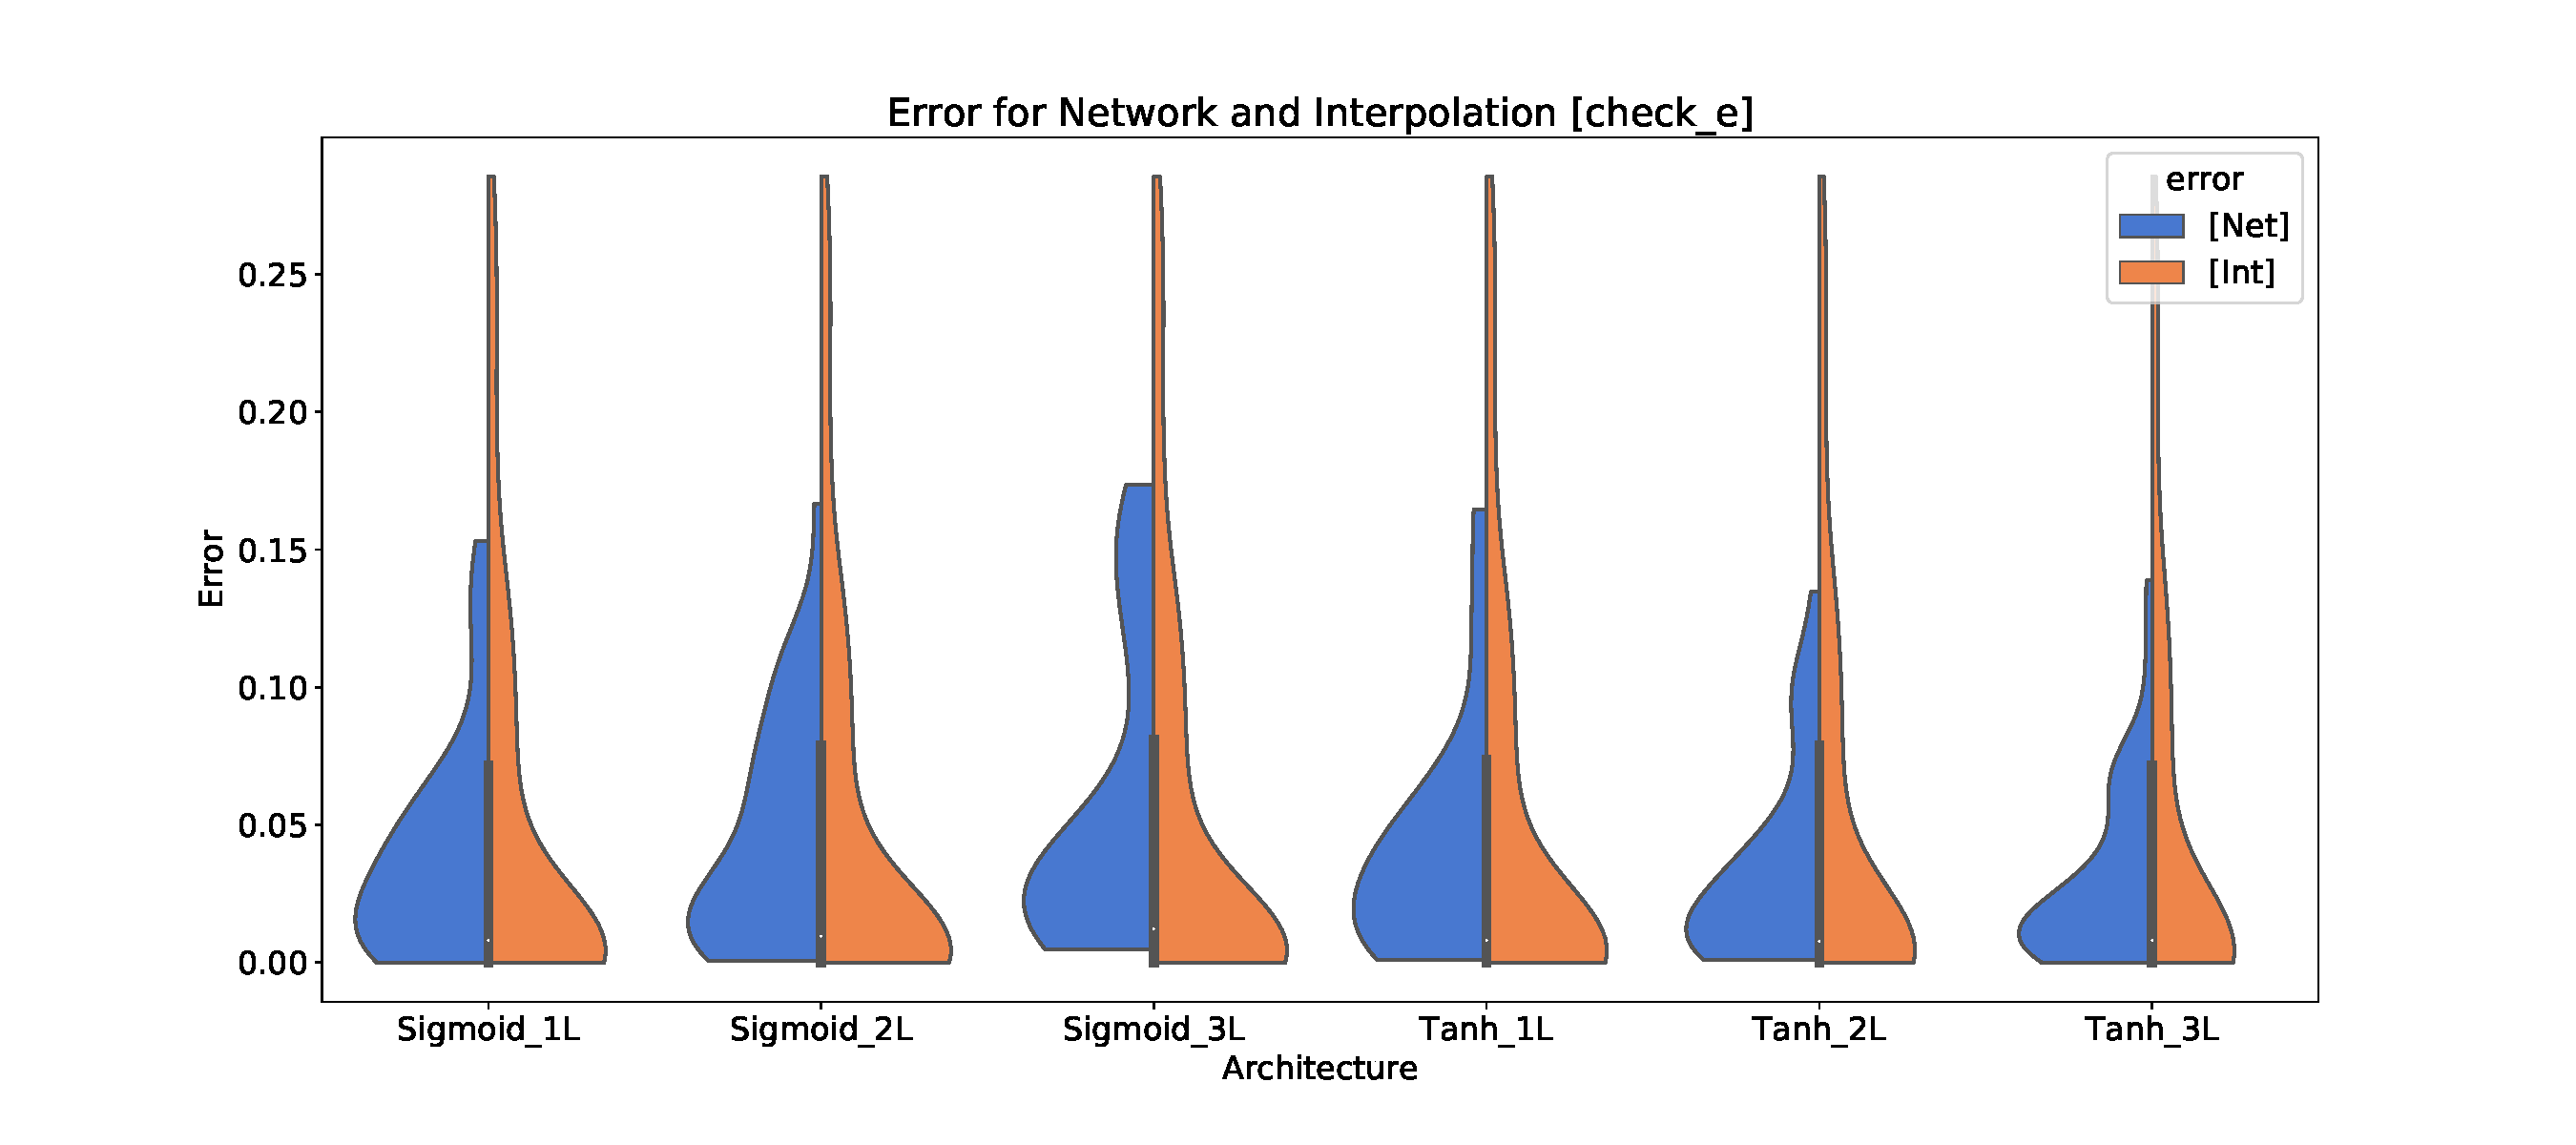
\includegraphics[width=\linewidth]{../figures/violin_plot_check_e.pdf}
    \caption{Violin plot dell'ellitticità valutata come rapporto tra le due FWHM.}
    \label{violin_check}
\end{figure}

%%%%%%%%%%%%%%%%%%%%%%%%%%%%%%%%%%%%%%%%%%%%%%%%%%%%%%%
%%%%%%%%%%%%%%%%%%%%%%%%%%%%%%%%%%%%%%%%%%%%%%%%%%%%%%%
%%%%%%%%%%%%%%%%%%%%%%%%%%%%%%%%%%%%%%%%%%%%%%%%%%%%%%%
%                   FINE CAPITOLO 3                   %
%%%%%%%%%%%%%%%%%%%%%%%%%%%%%%%%%%%%%%%%%%%%%%%%%%%%%%%
%%%%%%%%%%%%%%%%%%%%%%%%%%%%%%%%%%%%%%%%%%%%%%%%%%%%%%%
%%%%%%%%%%%%%%%%%%%%%%%%%%%%%%%%%%%%%%%%%%%%%%%%%%%%%%%







%%%%%%%%%%%%%%%%%%%%  CAPITOLO 4  %%%%%%%%%%%%%%%%%%%%

\chapter{Conclusioni}\label{conclusioni}
Alla luce di quanto esposto nei precedenti capitoli è possibile affermare che lo scopo di questa tesi è stato raggiunto. Ho infatti stabilito un criterio per discriminare la bontà dei diversi metodi di stima dei parametri del diagramma di radiazione. Tale criterio mi ha permesso di affermare che, con la giusta architettura, le reti neurali consentono di stimare i parametri di interesse più efficacemente rispetto ai metodi di interpolazione utilizzati.

\begin{comment}
Stai in pratica dicendo che lo scopo della tesi era di far vedere che le reti neurali funzionano meglio dell'interpolazione, ma questo non è un approccio scientifico. Lo scienziato dovrebbe porsi come scopo quello di valutare la tecnica migliore tra interpolazione e rete neurale. Lo "scopo che hai raggiunto" è quello di stabilire un criterio per discriminare la bontà tra diversi modi di fare regressione di parametri del beam (usando una griglia, dividendo tra training set e validation set, facendo grafici a violino), e questo è stato un successo; come conseguenza di ciò l'hai applicato a tre casi specifici (interp2d, curve_fit e reti neurali), e hai verificato che con questi criteri vincono le reti neurali. Ma la tua tesi sarebbe stato un successo anche se avessi dimostrato che interp2d era il migliore.
\end{comment}

Tuttavia il lavoro non è certo giunto al termine. La mia speranza è che questa tesi rappresenti un punto di partenza per ulteriori studi futuri. Ho mostrato che le reti neurali hanno potenzialità promettenti in questo ambito ma la ricerca sull'architettura migliore non la considero terminata. 
Per verificare se si possono raggiungere risultati migliori sarà di fondamentale importanza ripetere le analisi presentate in questa tesi con un database più ampio. I risultati potrebbero migliorare e potrebbero suggerirci se è necessario avere a disposizione un maggior numero di campioni  per effettuare il training della rete o se invece è necessario effettuare una ricerca più profonda sull'architettura di rete migliore.
Inoltre sarà estremamente interessante applicare la tecnica sviluppata ad un caso che presenti una diversa forma della superficie focale.
Uno sviluppo futuro riguarda senza dubbio l'applicazione del metodo di stima dei parametri del diagramma di radiazione attraverso le reti neurali a strumenti che presentano sulla loro superficie focale migliaia di detector e per i quali risulta infattibile una simulazione completa con i metodi classici (\ref{simulazioni}).


%%%%%%%%%%%%%%%%%%%%%%%%%%%%%%%%%%%%%%%%%%%%%%%%%%%%%%%
%%%%%%%%%%%%%%%%%%%%%%%%%%%%%%%%%%%%%%%%%%%%%%%%%%%%%%%
%%%%%%%%%%%%%%%%%%%%%%%%%%%%%%%%%%%%%%%%%%%%%%%%%%%%%%%
%                   FINE CAPITOLO 4                   %
%%%%%%%%%%%%%%%%%%%%%%%%%%%%%%%%%%%%%%%%%%%%%%%%%%%%%%%
%%%%%%%%%%%%%%%%%%%%%%%%%%%%%%%%%%%%%%%%%%%%%%%%%%%%%%%
%%%%%%%%%%%%%%%%%%%%%%%%%%%%%%%%%%%%%%%%%%%%%%%%%%%%%%%

\nocite{*}
\bibliography{../bibliografia/my_bib}{}
\bibliographystyle{abbrv}


\end{document}








